% \documentclass[12pt,final]{ucthesis}
\documentclass{ucbthesis}
\usepackage{biblatex}
\usepackage{graphicx}
\usepackage{amsmath}
\usepackage{url}

\usepackage{algorithm2e} 
\usepackage{lmodern}
\usepackage{amsmath,epsfig}
\usepackage{mathtools}
\usepackage{url}
\usepackage{xspace}
\usepackage{colortbl}
\usepackage{dsfont}
\usepackage{boxedminipage}
\ifx\pdfoutput\undefined
\usepackage[hypertex]{hyperref}
\else
\usepackage[pdftex,hypertexnames=false]{hyperref}
\fi

\usepackage{amssymb}
\usepackage{wasysym}

% \usepackage{caption}

\usepackage[caption=false,font=footnotesize]{subfig}
%\usepackage{subfigure}

\usepackage{listings}
\usepackage{color}

\definecolor{dkgreen}{rgb}{0,0.6,0}
\definecolor{gray}{rgb}{0.5,0.5,0.5}
\definecolor{mauve}{rgb}{0.58,0,0.82}

\lstset{frame=tb,
  language=Java,
  aboveskip=3mm,
  belowskip=3mm,
  showstringspaces=false,
  columns=flexible,
  basicstyle={\small\ttfamily},
  numbers=none,
  numberstyle=\tiny\color{gray},
  keywordstyle=\color{blue},
  commentstyle=\color{dkgreen},
  stringstyle=\color{mauve},
  breaklines=true,
  breakatwhitespace=true,
  tabsize=3
}

\DeclareMathOperator{\median}{median}
\DeclareMathOperator{\dis}{d}
\DeclareMathOperator{\mad}{MAD}


% Double spacing, if you want it.
% \def\dsp{\def\baselinestretch{2.0}\large\normalsize}
% \dsp

% If the Grad. Division insists that the first paragraph of a section
% be indented (like the others), then include this line:
 \usepackage{indentfirst}

%\newtheorem{theorem}{Jibberish}

\bibliography{references}

\hyphenation{mar-gin-al-ia}

\begin{document}

% Declarations for Front Matter

%\title{Metadata Management and Empirical Validation in the Built Environment Through Embedded Sensing}
%\title{A Framework for Sensor Data Processing and Empirical Verification \\for the Built Environment}
\title{A Platform Architecture for Sensor Data Processing and Verification in Buildings}
%\title{Design of A Platform Architecture for Sensor Data Processing and Verification in Buildings}
\author{Jorge Jose Ortiz}
\degreesemester{Fall}
\degreeyear{2013}
\degree{Doctor of Philosophy}
\chair{Professor David E. Culler}
 \othermembers{Professor Randy H. Katz \\
    Professor Paul Wright}
\numberofmembers{3}
\prevdegrees{B.S. Massachusetts Institute of Technology 2003 \\
  M.S. University of California, Berkeley 2010}
\field{Computer Science}
\campus{Berkeley}

% For a masters thesis, uncomment (remove the % at the beginning of)
% the following line.  This affects the title and approval pages,
% which by default calls this a "dissertation", not a "thesis".

%\itsamasters

% The title page generated by LaTeX is now acceptable for handing in.
% (This was not always the case).

\maketitle
\approvalpage
\copyrightpage

% (This is included by thesis.tex; you do not latex it by itself.)

\begin{abstract}

% The text of the abstract goes here.  If you need to use a \section
% command you will need to use \section*, \subsection*, etc. so that
% you don't get any numbering.  You probably won't be using any of
% these commands in the abstract anyway.

% Invasive brag; forbearance.



This thesis examines the state of the art of building information systems and evaluates their architecture in the context
of emerging technologies and applications for deep analysis of the built environment.  
We observe that modern building information systems are difficult to extend, do not provide general services for application development, do not
scale, and are difficult to set up and manage. 
We assert that a new architecture must be designed with four system properties -- \emph{extensibility, generalizability, scalability,
ease of management} -- in order to address these shortcomings.  
Our system, StreamFS, embodies these system properties through a filesystem abstraction and a set of data services.
% We propose a new architecture that embodies these system principles through a filesystem abstraction and data services, called StreamFS.  
Data services are made available to applications through an overloaded pipe abstraction.  This allows for dataflow specification
of processing streams to clean and analyze the streaming sensor data.

We deploy StreamFS in seven different buildings and compose several applications on top of it.  One of the driving
applications is a phone application called the Mobile Energy Lens.  The Energy Lens provides occupants with mechanisms for 
collecting building information
in a unified platform and provides a way to view aggregate energy consumption data associated with the spatial deployment configuration 
of plug-load devices.  We present a three-layer architecture, where one of the main layers is implemented entirely with 
the data management and processing services offered by StreamFS.  

We introduce the notion of verification of physical relationships through empiricial data.  
We partition the verification problem into three sub problems: 1) functional verification, 2) spatial verification, and 3) categorical
verification.  We show how empirical mode decomposition, correlation, and standard machine learning techniques can give us 
information about how the sensors are related to each other, statistically and physically.
We demonstate an \emph{extensible, generalizable, scalable, and easy-to-manage} system for supporting the ``appification'' of the 
built environment.  


% We examine the 
\end{abstract}


\begin{frontmatter}

\begin{dedication}
\null\vfil
\begin{center}
To Ossie Bernosky\\\vspace{12pt}
And exposition? Of go. No upstairs do fingering. Or obstructive, or purposeful.
In the glitter. For so talented. Which is confi∫nes cocoa accomplished.
Masterpiece as devoted. My primal the narcotic. For cine? To by recollection
bleeding. That calf are infant. In clause. Be a popularly. A as midnight
transcript alike. Washable an acre. To canned, silence in foreign.
\end{center}
\vfil\null
\end{dedication}

\tableofcontents
\clearpage
\listoffigures
\clearpage
\listoftables

\begin{acknowledgements}
I want to thank my advisor for advising me.
\end{acknowledgements}

\end{frontmatter}

\pagestyle{headings}

% (Optional) \part{First Part}

\chapter{The Vision of Soft Buildings}

We begin with a vision for the future of buildings.  We would like to turn all buildings into ``smart''
buildings that provide services to its occupants, the grid, and the environment.  Currently, buildings
are largely built in isolation of one another -- each unique in its own right, from the material the walls
are made of to the systems and software that control them.  With the falling cost of memory, the ubiquity of
connectivity and sensing, and cheap cost of computation in the cloud, it should be possible to make buildings ``smarter''
through software guided by the principals of extensibility and clean, well-defined software interfaces.

We would like to move towards a vision of building software systems that

\begin{enumerate}
\item Support the notion of applications; applications to make use of and directly control the environment.
\item Provide a clean set of abstraction for application writers that wish to build both analytical and control
applications.
\item Accurately capture the state of the building, even as it evolves.
\end{enumerate}


Recent trends in research and technology set the stage for our work.  We give a brief history of the work that has 
led us to the vision of a smart built environment.  We also describe the technology that
allows us to realize our vision and show how the falling cost of sensor, ubiquity of connectivity and embedded computation,
and falling cost of computation in the cloud informs our architectural choices.
In the next section, 
we discuss the built environment and how energy-efficiency has become a prime research focus.
Then, we give an overview of pervasive computing work and explain how they motivate the kinds of applications we look 
to support in the built environment.  Finally, we will state our research goal and give an overview of the rest
of the thesis.




\section{The Built Environment}
Humans spend a large portion of their lives in buildings and
there are known problems related to energy consumption, comfort, and operational visibility.  
Buildings consume 40\% of the energy produced in the United States and nearly three quarters of 
the electricity produced~\cite{epabuildings}.  With specter of global warming and the continued decrease in the cost of storage and 
communication, buildings have become a major target for improved energy efficiency.

Buildings have been the subject of study for architects, mechanical, and building engineers.  Recently, there has been an 
interest in buildings by computer scientists as they present a family of interesting challenges related to cyber-physical systems.
Historically, building manangers and contractors work together with a third-party provider to embed sensors through the systems
and spaces in the building to allow them to observe and manage
the day-to-day operations of the building from a central location.  The building manager is the primary user to interact with the
deployment information to diagnose and fix problems from a central locations.  Problem identification primarily occurs through occupant 
complaints.  The building manager diagnoses through physical inspection and simple inspection of the associated data through the primary
user interface for the \emph{building management system}.  These BMS's are common in large buildings.
Over 70\% of large -- 100,000 square feet or larger -- commercial buildings, have a building management 
system~\cite{cbecs2003}.  These systems are installed primarily for supervisory control and
centralized observation of the building.  
They help deal with the management complexity and supervisory control of a highly distributed mechanical system through
a graphical view and the sensors and actuators they contain.



% We assert that live and historical 
% sensor data must be exposed to application developers so they may build application that easily and continuously 
% asses the state of the building, identify faulty behavior, and enable holistic control.  


% We envision a future
% where buildings provide a standard way to observe and assess their operational performance, supports 
% the broad notion of programmability and enables the creation of different building applications, and 
% allows supports the suite of tools currently available for analyzing and controlling
% it.  We hope that future and to support emerging technologies that enhance these tasks.
% % We consider technological trends that set the stage
% % the work discussed in the thesis.  
% We examine problems in building with respect
% to energy efficiency and system maintenance and explore how computing can help. 


%   In order to optimize building performance, we need fine grained visibility into the energy flow
% throughout the building.  

% However, if you examine the infrastructure currently in place to provide this visibility you will discover tightly 
% integrated silos, bloated interfaces, and a lack of extensibility that is necessary to support broad 
% application development.  
\begin{figure}[h!]
\begin{center}
\includegraphics[width=0.5\textwidth]{figs/BuildingAppModel}
\caption{Building application model.  Building sensor deployments send data to the cloud and applications access it as it streams in.
Applications may also feed data to the cloud and make it available to other applications.}
\label{fig:buidlingapp}
\end{center}
\end{figure}



\section{Pervasive Computing}
The polifertation of cheap, networked, embedded sensors is moving us towards a future where our infrastructure is 
populated with computing that enable smart environments.  We march towards Mark Weiser's vision of the future of
computing \cite{uqicomp_vision} where the environment contains sensors and people interact with the 
physical environment through their personal devices and related services.  These services also allow us to 
optimize the performance of our infrastructure, uncover problems proactively,
and share information with others to provide greater insight into the world around us.  
% This vision is borne out
% incremenetally in the research community over the past 20 years.%since the vision was initially proposed over 20 years ago.

The research in this area starts from the vision for the field.  What could the world be if we are surrounded by computing?
How will we interact in that world?  What can we learn from the world and from each other?  Hypothetical scenarios
guide the early work.  A common scenario is one that makes use of a personal handheld device, ``smart'' objects, and 
ubiquitous connectivity.  Much of the early work aimed at constructing a scenario that captures some aspect of
the future envisioned that can be used to highlight and explore fundamental challenges in realizing the vision.
For example, Christensen et al.~\cite{Christensen_2002} explore how pervasive computing will play a role in assisting
office workers in their day to day activities.  They imagine a scenario where office occupants use their mobile devices
to interact and share information with each other through serendipitous work-related activities.  Through this scenario
draw attention to fundamental issues related to mobility, interrupted operations, and activity scheduling.% due to ad-hoc 
% collaboration.

Many fundamental challenges were discovered and addressed in this fashion.  Pervasive computing work eventually branched
off into several sub-domains with their own focus.  Some examples are work related to 
localization~\cite{Castro01aprobabilistic,Koo,Romer03thelighthouse,Yoon2013}, 
mobility and mobile devices~\cite{Haritaoglu:2001:ILR:647987.741331,Want02thepersonal,Jiang:2011:MPM:2030112.2030150},
context deduction and wearable computing~\cite{Holmquist01smart,Lukowicz2002,Christensen_2002,Rossi:2011:RWC:2030112.2030238},
and sensor networks~\cite{Conner:2001:MEL:647987.741329,Lymberopoulos09amethodology}.  These and related
topic areas have guided our thinking in addressing the problems in the built environment.

Looking back at the pervasive computing work, we observe that much of the work has focused on users but not as much on 
the challenges in the environment itself.  There is little
emphasis on the infrastructure and issues with the accuracy in contextual representation of the physical environment.
There is also very little work on how a changing physical environment affects the accuracy with which applications can 
deduce the state of the world around them.  Also, there is very little emphasis on control of the physical environment.
The kinds of software processes that runs in buildings are primarily for control of the environment.  These issues
are neither addressed in the building science community nor the pervasive and computer science community.  We look at these
issues specifically in this thesis.


% Through the construction of vision-style scenarios and application development in those settings, 
% frameworks emerged and fundamental challenges were uncovered. 
% The challenges and solutions are related to localization, contextual inference, multi-modal input, vision, and other issues.
% Eventually each of these branched off into invidual fields of study and communities that examined these
% more deeply.
% As these communities matured they were driven by more realistic deployment and application contexts.
% Over the years, this evolution has included advantaces in sensing, mobile, and network technology but also computational 
% ubiquity through cloud computing.  Moreover, as we consider problems that emerge in specific application domains or
% industries, we will see that the convergence of these technologies allow new domain-specific problems and solutions 
% to be explored.


% Much of the work in computing in the built environment comes from pervasive computing.  Over the last
% 20 years, researchers have explored how computation can be used to capture the physical environment and
% how applications can be used to combine computational resources into a coherent service for users.
% Localization is a fundamental issue addressed~\cite{Castro01aprobabilistic,Koo,Romer03thelighthouse,Yoon2013}.


% % \begin{itemize}
% % % There has been much emphasis on wearable~\cite{} and mobile computing~\cite{}
% % \item Applications for connected devices
% % \item Infrastructure and tools (the environment advertises services, devices compose them and present them)
% % \end{itemize}
% Smart Objects, Context Awareness, Wearable~\cite{Holmquist01smart,Lukowicz2002,Christensen_2002,Rossi:2011:RWC:2030112.2030238}

% Sensor networks~\cite{Conner:2001:MEL:647987.741329,Lymberopoulos09amethodology}.

% Mobile devices and mobility~\cite{Haritaoglu:2001:ILR:647987.741331,Want02thepersonal,Jiang:2011:MPM:2030112.2030150}.

% Much of the work has focused on user but not as much on the challenges in the environment itself.  There is very little
% emphasis on the infrastructure and issues with the accuracy in contextual representation of the physical environment.
% There is also very little work on how a changing physical environment affects the accuracy with which applications can 
% deduce the state of the world around them.  Also, there is very little emphasis on control of the physical environment.
% One of the primary kinds of software processes that runs in buildings are for control of the environment.  These issues
% are neither addressed in the building science community nor the pervasive and computer science community.  We look at these
% issues specifically in this thesis.


% What's lacking?
% > Little to no emphasis on the infrastructure that is already there for collecting informationa about the environment.
% > All the work is human-centric with general components.
% > No emphasis on issues with the data itself and how we can infer context while the context is changing in the physical infrastructure itself.
% 	> No talk about controlling the environment.  Mainly a focus on provided context-deducing/aware middleware and applications.


\section{Cloud Computing, Ubiquitous Connectivity, and Mobile Phones}
Cloud computing has changed the way we design systems that bring together the physical and computational world.  Coupled with the 
continued maturation of networking technologies -- both indoors through Wifi and outdoors through cellular -- and the explosion of mobile
phone use, today's systems are designed with the mobile phone as an access tool for information in the cloud.  It is mostly safe
to assume that this information will be accessible.  Moreover, connection speeds can reach up to 300 Mbps, so serving sophisticated
applications from the cloud and designing them in a highly interactive manner is commonplace.  The main bottleneck is the form of interaction, which
is still a challenge given the small screen of a mobile phone.

These technologies also make it easier to design centrally managed, globally accessible systems.  % into a single system that is centrally accessible.  
Services in the cloud
can serve many clients simultaneously, proving a unified view of the state of the service and the objects in it.  There is little difference 
between the desktop application and the mobile application, other than service presentation.  Moreover, all the data lives \emph{in} the cloud 
and is fetched \emph{from} the cloud by all clients.  The cloud service mediates interaction between all
participants in the system.

\section{Applications in Buildings}
% Advancements made in the pervasive computing communities, trends in technology, and problems in buildings lead us to thrust of this thesis.
We introduce the notion of building ``app-ification''.  Technology enables mobile phone ``apps''; mobile
applications that closely interact with content in the cloud.  We assert that a good way to address problem in the building
by opening up the building's sensor data streams and buildings services that make use of that data.  A system should provide 
\emph{uniform access} to the data and \emph{facilities for cleaning and aggregation}.  It should be \emph{extendable}
so disparite systems could join and share information that could enable new kinds of applications.  Figure~\ref{fig:buidlingapp}
illustrates a high-level of building ``app-ification architecture''.

Building-scientists and architects use a family of products and software packages that take building data 
and analyze it.  We need to support those as well.  The main idea is to expose building sensor streams and related information for 
applications through the cloud.  This allows us to adopt application development design patterns and inherit the benefits of 
centralized management.   It also provides an environment where a diverse set of applications and solutions can be designed
and tested to address fundamental challenges in building management and control.  %and a system where innovation can take place.
% We believe that the cloud-based service model would be effective.  
Such service should offer a data-processing primitives as well.   It should mediate access to sensor data and actuators.
The system should provide support holistic control applications that combine disparate data sources through the service itself.
We describe the design of such a system in Chapter~\ref{chap:SensingInBuiltMain}.


\section{Research Statement And Hypothesis}
We formally state the thesis that guides our work: %research thesis and hypothesis:
% \emph{What are the architectural components and technical challenges in the design of an information system
% that enables new and supports old classes of applications in the built environment?}  
\emph{How can we incorporate filesystem and database constructs and what are the technical challenges in a system that supports applications
in the built environment?}
Given the emerging applications in
the built environment it is clear that the old information system design is not sufficiently open, flexibile, nor
scalable enough to support them.  Old information systems are tightly integrated from the field-level sensor to
the central supervisor control system.  There are two integration points in traditional systems that we argue 
are either fundamentally flawed or insufficient for emerging applications.  We describe the components that 
currently exist and identify those that are missing.  We show how these components/services enable emerging applications.  We also
discuss the technical challenges that must be solved in order to provide the correct semantics for these services.
Furthermore, we discuss a component that is fundamental for providing correct information to applications 
and formalize the notion of verification in the context of the built environment.  We provide several algorithmic 
solutions to these problems, which lay the foundation for a fundamental service in the broader architecture.


\section{Thesis Roadmap}
In the next chapter, we discuss building information systems today.  We dive into their architectural components and introduce some terminology
used in the building space.  We also describe the motivating scenario that they were built for and examine how well the architecture 
can support the ``app-ification'' of buildings.  We give examples of specific applications that we would like to support
and walk through the components that are useful for this purpose and those that are missing.  We propose a set of necessary
components in an architectural re-design that could provide the same support as BMS's today as well as the emerging ones that we
describe and argue that this should be the design of a \emph{building appification system}.

In chapter~\ref{chap:SFSArchMain}, we give an overview of a system that contains the components we propose in the previous
chapter.  The name of the system is StreamFS.  StreamFS is a cloud-based service that combines filesystem and database constructs
to organize the streaming sensor data, clean and process streams, and provides a unified access layer.
%  for both physical information
% and actuation channels in the physical world.  
We discuss the overall structure each component in the architecture and how they interact with one another.

Chapter~\ref{chap:mechanisms} dives into the details for the components and mechanisms in StreamFS.
Section~\ref{sec:promngt} focuses on the process management component in StreamFS.  The process management component
manages the streams and the processes that consume those streams.  It is designed to support processes that are specified by the user
and managed by StreamFS as well as integrating external processing components and representing them through the file system in StreamFS.
We discuss some of the challenges and present some solutions to a scheduling problem related to providing fresh data  to processing jobs.
We also describe how various kinds of aggregation can be performed on the data, using the filesystem and pipe abstraction
presented and managed by this component.
Section~\ref{chap:naming} discusses how we represent the world as a collection of files.  StreamFS follows the unix filesystem principal 
where everything is a file and this allows us to provide a unified management layer for the entire set of building deployment
data and metadata.  We discuss the individual file types that we support and their semantics.  We also introduce the fundamental
challenge of dealing with evolving metadata.  Specifically,  we show how changes in the physical world can present problems
with the structure and relationships between the files in the system.  
% We show the basic set of tools that we use to address these problem
% at the end of the chapter.

We evaluate the StreamFS in chapter~\ref{chap:ArchEvalMain}.  We describe our experience in deploying StreamFS in several buildings
at UC Berkeley and the University of Tokyo.  We describe these deployments in the context of 2 applications: 1) a real-time visualization and 
aggregator mobile phone for energy auditing, and  2) a real filesystem mount and direct integration with a legacy applications. 
We also give an overview of the application programming interface and discuss how StreamFS can help build generable, scalable 
re-useable software within buildings.

Finally, we discuss verification of building systems and metadata in chapter~\ref{chap:VerificationMain}.  We introduce 3 types of 
verification and describe why each of them is crucial to building applications that interact with the physical world through
a layer of software represent it.  We discuss our work on the Strip, Bind and Search methodology for functional verification, 
our use of mode decomposition for spatial verification, and timeseries clustering techniques for type classificaiton.  
We discuss future work in chapter~\ref{chap:future} and conclude in chapter~\ref{chap:done}.





























\chapter{Sensing in the Built Environment}
\label{chap:SensingInBuiltMain}

% Buildings consume nearly 40\% of the total energy produced in the United States and 72\% of the electricity.  Similar figures 
% have been recorded in other industrialized countries~\cite{buildings_study}.  Furthermore, studies show that they waste from
% 30-80\% of the energy they consume.  

Building management systems consist of thousands of sensors embedded in the systems that control the internal environment and
the spaces occupied by people.  Many different sensors take disparate physical measurements, continuously.
For example, temperature sensors take Fahrenheit readings in the thermostats,
valve-position sensors measure the position angle of the valve in the pipes, pressure sensors record pressure measurements in the vents, 
etc.
% temperature sensors on the vents and pipes as well, etc.
The BMS presents these through a graphical interface to the building managers.  The graphical interface contains graphical sketches
of the systems and spaces in the building with icon images of the sensors in their approximate physical location represented
in the sketch.  The image sketch is generated from building schematics, so the interface is representative at the time of construction.
Building managers can quickly locate any sensor in the building through a series of clicks.

% that is giving bad readings or find the sensors that support
% a space where complaints are coming from, so that he/she could identify faulty readings through close inspection.
% The interface also allows them to visually inspect and quickly try to diagnose a problem, typically in response to occupant
% complaints.

Although BMS's have, to some degree, been an effective tool for centralized management of buildings, they lack the extensibility
and analytical capabilities necessary to support an ecosystem of tools for analyzing the building.  In general, software
practices in the building are non-standardized and non-systematic.
% Although BMS's have been revolutionary from a building management perspective, they lack many fundamental components for
% the kind of analysis that is needed to understand the building's operation over time.
% is performing now  
% and will perform in the future.  
% Also, building practices for software-driven building systems serve more as guideline than
% as a standard.  Naming, access, and organization of building data varies as much as buildings do.
This presents major challenges with respect to software re-use and scalability.  
In this thesis we discuss how we address these challenges through architectural design choices and analytical methodology.  
The architectural choices reconstruct the software layer that sits on top of existing building management systems and presents
a unified interface and standard API for analytical and control building applications.
The analytical methodology offers a general approach for verifying the construction of point names -- the naming scheme for 
sensors distributed throughout the building.  
% Both set a foundation for ongoing and future work.

The thesis is presented in the context of BMS systems and the building applications we aim to support.
% building systems and building-related applications.  
% We draw out the components in our analysis and design and discuss where it fits in the broader context of prior, computer-science related
% literature.  
In the next section, we describe the state-of-the-art practices followed by vendors of building information systems.
We describe the architectural features and design principles both implicitly and explicitly implemented into them.
We also present the pros and cons of these decisions and their implications and include a high-level description of our approach.
% Later chapters delve more deeply into the implications of our design decisions.

\section{Tightly Integrated Building Information System Architecture}

The first building information systems became commercially available in the 1970's ~\cite{gardner1987energy}.  
Historically, building management 
systems were constructed as a collection of control loops, which progressed from pneumatic to analog to digital.
These control loops largely form the foundation for the design decisions made in building information systems.  
This section gives a quick overview of the architecture, bottom-up and describes how each stage is built around
the concept of loops and supervisory control.  We then describe some of the short-comings of this architecture
and give an overview of how we address it in a system called StreamFS -- described in more details in
the remaining chapters.

\begin{figure}[t!] %htbp
\centering
\includegraphics[width=0.50\columnwidth]{figs/control_loop}
\caption{General building control loop.}
\label{fig:control_loop}
\end{figure}

\subsection{Control Loops and The Outstation}
\label{sec:control_loops}
Each loop is defined by a control domain consisting of a sensor, an actuator, and a control mechanism.  The control mechanism
become logic based when signals from sensors moved to the digital domain.  However, the basic control principle is based
entirely on local control loops, with the implicit assumption that these loops are independent.
Figure~\ref{fig:control_loop} shows a high-level control loop.  A simple control loop in the building is one that controls
the temperature in a space.  It has a temperature sensor as the input and uses the temperature set-point parameter to 
decide when and which actuators to activate.
For temperature control, this actuation controls the the vent that lets cool air into the space.  This causes the temperature
to fall until a lower-bound is reached and the control logic re-activates the fans and heating/cooling system.

The figure also shows the basic structure inside an outstation.  An outstation is a box that contains up to several control boards, each
wired to one or more sensors and one or more actuators.  The outstation is typically close to the sensors and actuators (in the same room)
and contains all the control logic for the local plant.  Inside the control logic there is a CPU and some memory.  The memory
contains the control program and some space for sensor readings.  It is directly wired to the sensors and actuators through
a series of buses and shown in Figure~\ref{fig:control_box}.

\begin{figure}[t!] %htbp
\centering
\includegraphics[width=0.50\columnwidth]{figs/control_box}
\caption{High-level control board architecture.}
\label{fig:control_box}
\end{figure}

As readings from the sensors are taken, they are placed in RAM.  The amount of RAM is limited and can get filled up, so it is important
to schedule periodic collection tasks from the central station -- the building management system (BMS).  The control logic is typically
written in ROM and can only be changed by the equipment or BMS vendor.  The input parameters are set at the BMS and they dictate the operational dynamics
of the control scheme in reaction to the input~\cite{BMS_book}.
Outstations are distributed through the building and are essentially running independent of one another.  In order to enable centralized 
monitoring and control, they are networked together and report some of the sensor readings and control-logic state to a central outstation.

\subsection{Central Outstation and Communication Protocols}
The central outstation is typically a Microsoft Windows-based PC connected to the outstation through either RS-485/modbus or Ethernet.
The user interacts with the system through a graphical interface, constructed from the schematics for the building or the schematics
for the component in the system that is being monitored.  The BMS running on the PC communicates with outstations through either a 
vendor-specific, proprietary protocol or an open one like BACNet~\cite{Bacnet} or LonTalk~\cite{LonTalk}.  Note, 
we focus on BACNet, but the similar features exist in other protocols, such as LonTalk.  

\begin{figure}[h!] %htbp
\centering
\includegraphics[width=0.50\columnwidth]{figs/BMS_network}
\caption{High-level control board architecture.}
\label{fig:bms_network}
\end{figure}

Both protocols define both a wire protocol and packet structure for communicating with outstations and each other.  They also define a high-level
naming scheme for sensors in the building, called `points'.  A point can also refer to a non-physical object, like a schedule of operation.
It is common for both lights and temperature sensors to run on a daily, weekly, and seasonal schedules.  Such schedule are captured
by the \emph{schedule object} in BACNet.  
% BACNet also exposes devices as a collection of different object types.  
Each object contains a set of properties that can 
be read and/or written.  A device is identifiable through a name or address on the network, each object has a unique identifier and is one of
many types.  Examples of object types includes the following: input, output, value, analog~\cite{Bacnet}.  

These protocols also provide a mechanism for discovery .  Each [device, object name/id, property name/id] tuple forms a name.
This name is exposed by the protocol-server to the application.  All the names are set by the vendor and the are shown through the graphical interface
of the BMS.  
% constructed from the building schematics, is also designed and constructed by the vendor.  
The building manger is the primary user of the BMS,
so rather than expose the underlying protocol, he/she interacts with the building via the graphical interface.

In order to interact with the underlying sensor and actuator layer, the application must use a stub that communicates directly with the 
sensor/actuator through the BACnet stack.  External communication stubs are recognized similarly to sensors/actuators.  They are represented 
as a collection of 
objects with readable/writable properties.  An example service that is provided in BACNet is  \texttt{WhoIs} and \texttt{EventNotification}.
The former is a broadcast service that is used for discovery of other objects, the latter is used for setting alarms on the sensor data that
are reported by the BACNet enabled devices on the network in the outstation layer.  There are many other types of events that are supported 
and over 50 types of object types in the baseline protocol, which is extensible.  Device and object names that are added have no restriction
on either the number of characters (specified by the vendor) or the encoding.


\begin{figure}[t!] %htbp
\centering
\includegraphics[width=0.25\columnwidth]{figs/bacnet_device}
\caption{BACNet device example.}
\label{fig:bacnet_device}
\end{figure}
\section{From Supervisory Control to Application Development in Buildings}
%From Supervisory Control to Application Development in Buildings

% Building information systems were built as tightly integrated silos, where the main application is the graphical user interface.
Features for interoperability were designed at two interface layers: 1) the protocol layer and 2) the presentation layer through a
data-export feature.  The protocol layer provides services for enabling devices to talk to one another through the network.  
Several features were explicitly designed around
the notion of interoperabilty: trending, scheduling, management services, alarms and events, direct sharing.  The graphical
interface layer is mainly focused on providing periodic reports in a comma-separated value (CSV) file, which
contains point-name information and time-value pairs of data.
% Historically, the extent of interoperability objectives has included mainly the introduction of new devices onto the network or
% the exporting of data for other software program to use for analysis and report generation.  
For these protocols, interoperability means adding new devices or exporting the data in a common format.
Building informtation systems themselves
were built to mainly support the in-time management and supervisory control of the building.  Analysis does not 
extend far beyong univariate plotting and individual assessment of equipment and control.  Most tuning of control parameters is 
manual.  Hard-wired control logic at the outstation is rarely updated.


Over the last few years, however, there has been in increased interest in energy management and comfort as a primary objective 
in the design of new building applications~\cite{6146507,Yu1956572,Mamidi2343582}.  Moreover, there is a broad interest in buildings
using global control schemes to optimize their performance and to interact more efficiently in response to renewable sources and its  
generation volatility~\cite{Taneja2223873,5985456,Lu2009}.  Model predictive control has introduced new ways of controling the components in the building
to make them more energy efficient~\cite{mpc}, there is an interest in performing dynamic, real-time analysis of building health
and efficiency~\cite{dynamicLeed}.  There has even been interest is improving the visibility of the state of the building to the 
occupants through various modalities, including touch-screens and mobile phones~\cite{andrew_lighting, Hsu1878444, Ortiz2422540}.  
These, and other emerging applications,
have pushed the boundaries of demand beyond what a modern building information system can provide and a re-design must be considered.
\section{BMS Architectural Shortcomings for Supporting Emerging Application Development}

\begin{figure}[t!] %htbp
\centering
\includegraphics[width=0.75\columnwidth]{figs/soda_bms_screenshot}
\caption{Screen shot for the Soda Hall Building Management System Interface.}
\label{fig:soda_bms_screenshot}
\end{figure}

% In this section we dissect the current architecture in the context of current and future applications
% for buildings.  The first two describe how the current architecture is used to provide the intended service
% that these application provide.  The latter two are emerging applications that we would like to available
% throughout the entire building stock.  We will see, however, that these are very difficult to build at scale
% and we pose the question ``what is missing in the current architecture to enable the system properties that help
% support these and other emerging applications?''.  Through close inspection it will hopefully become clear that
% the current architecture is fundamentally flawed; built largely to support a small set of vendor-specific
% applications and not much else.

% In this section we dissect the BMS architecture and closely examine how well it can support broad application development
% in buildings, rather than the single supervisory control function it supports today.  
We examine today's BMS architecture in the context of 4 potential services with distinct operational requirements. % that need to be supported.  
The first two services are features in today's BMS's.  
We describe how emerging requirements are driving the evolution of these
services and how BMS's are struggling to meet the new requirements due to limitations in their architectural design.
The next two are emerging services that BMS's cannot support today.  We describe which architectural components must be included
or how current components must be modified in order to support these.  We also make the broader argument that 
building systems should be built to support a much wider range of applications that we cannot currently anticipate.
We will show why this requires a fundamental re-design and propose an architectural composition for such a system.
In the rest of the thesis, we will examine an instance of our architecture and describe the challenges in realizing
the use and effectiveness of our system in real building deployments.

% while the latter are potential applications we imagine will be supported in future
% smart buildings.  Through this exercise, we build our argument for a systematic re-design of such systems and propose
% a set of necessary architectural components necessary to enable and support emerging applications.

\subsection{Monitoring and Supervisory Control}
The primary objective in the design of building information systems is for centralized monitoring and supervisory
control.  Control algorithms are left ``to the expert'' and embedded in the outstation control board.  The intended
user of the system is a building manager -- a user whose expertise is much broader than the designer of the control
algorithm that runs on a particular system component.
The manager is expected to monitor the health of building systems and quickly diagnose problems when they occur.  The tool
is mainly in place to save the building manager time; and it is very effective at doing so.  The extent to which 
the building manager is making control decisions is altering control algorithm parameter setting through
the building management interface itself.  Even these decisions typically go through the vendor, through consultation.

Figure~\ref{fig:soda_bms_screenshot} shows a screenshot of the BMS in Soda Hall at UC Berkeley.  This specific image
captures a schematic for one of the air handling units.  It shows the various sensors embedded in different locations
on the component -- temperature sensors on either side of the supply/exhaust fans, temperature sensors at the supply/return 
air ducts and the inlet vent, measuring the outside air temperature.  Accompanying real-time readings are juxtaposed
by the sensor image.  The user can double-click on the sensor or reading to get more information about that particular 
measurement point.  For example, if you double-click on a temperature sensor, it will give you the exact name of the 
point and accompanying information about related points, such as the set-point, which effectively drives the behavior of 
the underlying system.  If an occupant makes a complaint about not getting any air from the vents, for example, the 
building manager can find the screen for the vents that serve the room the occupant is in and observe the current
pressure readings or look for value-based alerts on any of the readings, typically displayed on the same screen.
If there is a malfunctioning component or something stuck in the vent, the readings should ``look off'' to the building 
manager.

If the problem recurs often, the astute building manager may be able to characterize the fault through a series of alarms.
They can be proactive about finding and fixing the problem(s) before they occur.  Alarms can be set through interaction
with the graphical interface, in much the same way that a look up on the measurement point occurs -- by double-clicking on 
the point in question and following instructions for setting an alarm.  In some cases, the problem may be driven 
by a faulty setting and adjustments can be made to the control parameters through the associated control points.

The scope of control is limited to local control loops.  Recall our discussion of control loops in section~\ref{sec:control_loops}.
The building manager can, typically with the help of the vendor, decide on the best control strategy setting.  If the control
strategy cannot be met, due to flaws in the control algorithm itself, the vendor may step in and re-image the controller
at the outstation and expose the necessary parameters through the graphical interface.  These kinds of changes are rare
but do happen occasionally and are generally expensive, since the cost is not usually included with the purchase
of the system.  The decision is made after close inspection and analysis, which a BMS enables through the data export feature.  
For example, the sense/control points in question may be placed in ``trend'' mode.  This means that readings
from those streams are stored in the local memory buffer at the outstation for some period of time.  If a report is specifically
set up at the central system, a report period is associated with the point of interest. This allows the saved data to be drained
from the local buffer at the outstation.  The data are written in a file for observation and graphing by the 
building manager.  %Time-dependent inspection of the behavior of any of the control-loop related points can be examined.

Although this feature is not necessary in order to change control parameters, it is useful for observing how parameter changes
affect the behavior of the system.  The building manager can, in principal, experiment with different setting and allow
empirical observations to guide her future decisions.


% Buildings waste as much as 30-80\% of their energy~\cite{waste_science, next10_waste}, have little agility
% to adjust to outside factor, and each one is unique from the mechanical system to the BMS.  This motivates
% the research presented in this thesis.  

\subsection{Energy Auditing and Building Modeling}
\label{sec:elensvision}
Recently there has been renewed interest in the energy consumption of buildings.  In particular, several studies~\cite{BuildingEnergyData,
MITBuildingScience} show that buildings consume a large fraction of the energy produced in the United States and that as much
as 80\% of it is wasted\cite{waste_science, next10_waste}.  As such, there has been an emergence of several companies and 
services for assessing the health of
commercial buildings with respect to their energy consumption.  Organizations such as LEED~\cite{Leed} provide certification of 
buildings, specifically rating the energy efficiency of the building.

Building modeling software, such as EnergyPlus~\cite{eplus}, are used extensively by building scientists. 
EnergyPlus and simulators like it are part of an ecosystem of software that models various aspect of the operation
of the building.  They allow the designer to construct detailed models of the building, from construction materials to 
operational usage and occupancy.  Some parameters include
construction material, longitude and latitude, zone-based usage (office building, bathroom, storage room), window size, etc.  
There are literally thousands of parameters that can be set.  All LEED certification relies on the construction of an 
accurate model that demonstrates energy efficient performance.
% Typical certification requires the submission of the detailed
% model and the results of various energy-related metrics, aggregated over seasonal time intervals to attain LEED certification.

Model construction can take several months.  In order to construct an accurate model, model output is compared with
empirical data.  Most BMS systems provide a way to export the  trended data.  
The file export feature and the ability to ``trend'' points, serve as an interface applications.
Another option is to obtain the data directly from the system through the network.  Third-party vendors provide systems that 
will join the building network of devices and eavesdrop on the network for sensor data reports.  % and traffic being reported to the central server.
In many instances, this is the only way to obtain truly real-time readings from the sensors on the network.
BMS vendors do not like this, since they such devices may generate traffic that overwhelms the network.  % because of congestion.
% Although not fundamental, it is a common concern in building sensor networks.  
Many buildings use RS-485 rather than Ethernet and there is
a general, albeit unfounded, concern that the network will become overwhelmed if all the points are trended and report 
simultaneously.

Modeling and real-time analysis have been separated because of these constraints.  The constraints are largely not
fundamental, but the current architecture is simply not designed to provide real-time readings for \emph{all the points, simultaneously}.
Also, it is clear, even from the fairly simple workloads generated by these analysis applications, that a history of readings
is needed.  BMS's, as currently designed, require the end-user to manage the history of the data point individually.
When BMS's were first designed, there were certainly concerns about bandwidth and storage limits.  However, today those concerns
are a non-issue.  A few hundred bytes produced on the order of minutes, even from several thousand sensors is simply not
that much data.  For example, 10k sensor produces readings every 15 minutes at 200 bytes per report is only 
17 Kbps.  Even if the streams are synchronized, the total amount of data is 2 MB.  Ethernet links and switches can handle Gbps 
transfers.


\subsection{Holistic Building Optimization}

\begin{figure}[t!] %htbp
\centering
\includegraphics[width=0.75\columnwidth]{figs/mpc1}
\caption{Emerging Application: Hierachical MPC for a stock of buildings.}
\label{fig:mpc1}
\end{figure}

An emerging class of applications, is in holistic control of the building using a new technique called model-predictive control~\cite{MPC_yudong}.
Rather than rely on specific changes to control logic at the local-loop level, MPC techniques observe and learn a model
of the behavior of a components, multiple components, or the whole building, based on the historical data.  Once the model is learned, 
constraints can be specified to drive the behavior of the system to an optimal region in the trade off space; solving it as 
a constraint optimization problem.  Figure~\ref{fig:mpc1}, reproduced from~\cite{MPC_yudong}, shows an example of hierarchical MPC control.  
It decomposes a large optimization process -- High-level MPC --  into individual control decision to be made at the control-loop level --
low-level MPC.

In order to enable the low-level MPC, the process must know the mapping between the points and their location.
The user must connect the right data streams and control points to the algorithm's inputs by either manually going through the schematics or
locating the schematic representation in the BMS graphical interface.  There is no query interface to a BMS.  This task requires sitting 
with the building manager or vendor in order to set up the trending, reporting, and enabling the necessary control permisions.
Needless to say, it is very time consuming and \emph{does not scale}.

% Although the method is very useful and has yielded excellent results, it is difficult to replicate.   
% The code and setup must be 
% customized for each building or stock of buildings it is set up on.  
This lack of generalizability and scalability hinders widespread deployment of innovative solutions.  In most cases the 
mapping of sensor/actuator to their placement in space/system are 
captured through in a combination of the schematics, the graphical interface, and the point name. Moreover, buildings are 
are one-off constructions and their associated digital information has followed the same pattern.  Although MPC can yield significant savings, setup complexity and building uniqueness, makes it nearly impossible to replicate quickly.  It is fundamentally difficult to generalize. 


\subsection{Personal Energy Viewer}
\label{sec:mobile}

\begin{figure}[h!] %htbp
\centering
\includegraphics[width=0.75\columnwidth]{figs/mobileEnergy1}
\caption{Emerging Application: Mobile phone interfacing with the physical infrastructure.}
\label{fig:mobileEnergy1}
\end{figure}

Imagine having the ability to walk through a building and see live, detailed energy data as
you point your phone at various things and locations.  As you enter the building, you scan its tag and see
the live breakdown of energy consumption traces, including HVAC, lighting, and plug-loads.  You continue
your walk through the building as you head to your office.  When you arrive to your floor
you scan the tag for the floor and observe similar figures, only this time they are in relation to that floor
alone.  Since there are several meeting rooms on that floor, you are curious how much is consumed by 
occupants versus visitors.  You choose to view the total load curve co-plotted with the occupant
load curve, specifically for that floor.  You see that approximately half the total energy is consumed
by visitors during the day.  

Curious about what portion of total are attributed to you, you select the 
personalized attribution option and you see \emph{your} personal load curve plotted
with the total load curve -- as well as accompanying statistics, such as the percent of total over time.
As you quickly examine the data on your phone, you see that you consumed energy during hours that you were not
there.  You choose to see a more detailed breakdown.  You enter your office, scan various items that you own, and see that
your computer did not shut down properly and your light switch was set to manual.  You immediately 
correct these.

Being able to interact with your environment and get a complete energy break-down can provide a useful tool
for tracing and correcting rampant energy consumption.  In buildings, having the occupants actively participate
allows for localized, personal solutions to efficiency management and is crucial to scaling to large buildings.
However, providing this detailed level of attribution is challenging.  There's lots of data coming from various systems 
in the building, and integrating them in real time is difficult.  Furthermore, attribution is non-trivial.  
We must be able to answer to following: How much of the total consumed on this floor went to charging laptops?  How
many of those charging laptops belong to registered occupants of this floor?
For centralized systems, multiple locations are served simultaneously.  It is non-trivial to determine the exact
break-down for each location.  At the plug-load level, some plug loads move from place to place throughout the building
over the course of the day.  Tracking where they are at any given time is difficult.

Answering these queries is relatively easy once the information is available, however, collecting the information
is non-trivial, especially over time.  Historically, it has been difficult to collect plug-load information.
Various studies have used wireless power meters to accomplish just this~\cite{stephscale, lanz, aceee}.
All previous work collected the data and performed post-processing to analyze it.  We want to take the next
natural set of steps: perform processing in real-time and present the occupants with live information.

Currently, in order to enable this application, a detailed digital model of the building is necessary, data streams from the building must
be easy to query, and it should work across buildings.  Also, there needs to be a way to localize the user. 
Localization technology and information must be made available to the mobile application to provide in-situ services.
It's clear that the current information infrastructure cannot provide these.  The interface to the network does not have
a strict naming mechanism, there is not explicit representation of each building that the application could interpret, 
the sensor/actuator deployment is not dense enough and adding new sensor is cumbersome.  Furthermore, the data itself can be quite dirty.

Cheap sensors are unreliable.  They produce erroneous data and randomly stop and start at times.  Missing/erroneous data is common.
Moreover, within building information systems provided by a single vendor, there is no time synchronization across sensors, so
aggregation, filtering, and re-sampling are common operations that must be performed on the data in order to summarize and display it.
The mobile energy viewer application not only require these but requires that they be performed in real time.






\section{Addressing BMS Shortcomings}
The current architecture of building information systems is very tightly integrated and based on monitoring and supervisory control
of local control loops.  Building information systems were built as tightly integrated systems with a single application.  The main
layer of interaction is been the underlying network layer.  However, because of the complexity of dealing directly with the network,
later iterations of BMS's included an export feature which decoupled the protocol from the necessary information, namely, time-value
pairs for each point in the system.  As auditing applications emerged and energy became a prime target for reduction in buildings, 
these interface choices became overloaded.  Moreover, as the need to build new kind of applications emerges, the architecture pieces
that are missing become more clear.  The following is a list of some of them:

\begin{enumerate}
% \item Network protocol details should remain opaque to end-user applications.
\item Narrow waist should be above the network layer.
\item A time-series store is necessary.
\item Mechanisms to distill the readings must be availble.
\item Real-time data forwarding should be available, especially for control applications.
\item Contextual relationships between sensor should be verified.
\end{enumerate}

The first four items are commonly built and re-built in emerging applications.  Therefore, we argue that they are fundamental 
to the future architecture of building information systems.  Moreoever, we observe that dealing with network-protocol specific
calls is not only cumbersome, but usually circumvented in order to deal directly with the data.  Most applications that do
use the underlying protocol expose a name-time-value (NTV) tuple to the layers above.  This observation leads us to believe that
that's where the interface should be.

The NTV layer also allows us to decouple of the data from the network protocol.  This makes it easier to include 
new sensors that may not be directly on the building network.  For example, wireless plug-load power meters~\cite{ACme}
can simply join the NTV layer by registering the individual points, while a translation layer between the NTV layer and the
main router can provide the transformation of read/write request to/from points in the network.  The same is true for BACNet
or any point protocols for sensors/actuators.

Each of the services that require the end user to have a deeper understanding of the underyling dynamics or performance
of the building \emph{must} capture the notion of time.  Almost all anlytical process or control decision needs a set of readings
over time.  Therefore, there a time-series data store must be part of future BIS design.  The service should be made available
through the NTV.  This will allow applications to fetch the necessary data for analysis either for display or complex processing.

The third point is motivated by the observation that sensor data, especially from cheap sensors, is dirty and typically goes
through a cleaning process before being forwarded to the end-use application.  There are various operations that are commonly
performed on the data, that we think should be provided as primitives.  These mainly include re-sampling, filtering,  
missing-data identification, and aggregation.  Re-sampling refers to taking a set of streams and interpolating missing values to 
align their timestamps.  This is typically performed before aggregation, especially for generating time-varying aggregate statistics.
Filtering simply refers to the removal of certain values based on some criteria of acceptance.  Usually the criteria is defined
by a threshold, both lower-bound and upper-bound value threshold for a particular stream or set of streams.
Since data is often missing, due to intermittent connectivity problems or faulty sensor equipment, it becomes important to 
get a summary of missing time intervals in order to adjust the fetch parameters.  Finally, the data is usually more
useful in aggregate than as a univariate signal, for example, for generating a load curve for a set of energy-consuming items.
Simple operators for combining values of various streams is key to enabling this analysis.

Finally, in order to enable control, real-time mechanisms must be exposed to the control application, while maintaining the 
layered integrity of the NTV layer.  In addition, we have observed the need to provide real-time services for analytical applications
as well.  For example, LEED is now proposing the use of building data to provide a dynamic performance meter~\cite{DynamicLeed}.
There are also many dashboard companies that make use of streaming data to provide real-time statistics on the performance of the
building.  The mobile application described in section~\ref{sec:mobile} also requires a real-time forwarding and processing service to
enable the application.  We believe that as more applications emerge they will likely need make use of real-time sensor data.





\section{Contextual Accuracy}
\label{sec:cntxtacc}

% There is yet another, more fundamental aspect of the architecture that we have not discussed, namely, contextual accuracy.
Contextual accuracy is the notion that the context -- physical location, type, etc -- about the data we are analyzing, must be accurate
to interpret the results for the analysis accurately.  For example, an application that is providing aggregate statistics on the 
power consumption by plug-load items on each floor of a building, must be sure that all the data used for the analysis 
is power-meter data on the specified floor.  If power meter A on floor 1 is moved to floor 2, the code doing the aggregation
should discover the change and adjust the aggregates for floor 1 and floor 2.  Another example is related to model predictive 
control processes that assume contextual relationships among a set of sensors to derive the state of a physical space and 
make control decision that affect that state.  If sensors are update, moved, added, or changed, the queries made by such processes
will be inaccurate and lead to incorrect control decisions.  Many such processes will exists in future smart buildings, so
automating the verification process as much as possible, is crucial.
% This example may seem contrived, however it is a
% more general example that has to do with the verification of the underlying metadata/tags associated with the stream names.

All of the metadata for each point is inputted by a human being.  Given the scale of the task -- thousands of sensors per building --
it is highly error prone.  So what may seem like a trivial problem for a single instance (as described above) leads to gross
miscalculations at scale, in the number for points and in time.  The building and the deployment within it go through a natural
evolution and this will impact processes that depend on knowing the context of the readings in order to make the right automated decision.

\begin{figure}[h!] %htbp
\centering
\includegraphics[width=0.5\columnwidth]{figs/mpc_example}
\caption{MPC example where metadata must be verified to maintain correct behavior.}
\label{fig:mpc_example}
\end{figure}

Figure~\ref{fig:mpc_example} shows an example where this will have a more direct impact.  This example shows a simplified illustration
of the relationship between a chiller and a space in the building.  The building of the future will optimize the space using a 
model-predictive control strategy (MPC) based on Equation~\ref{eqn:room_temp_control}.  The equation is used to model the temperature
dynamics of the room.  In this equation C is the termal capacitance (a constant), T is the temperature in the space, u is the heating/cooling
power input, $P_{d}$ is the internal load, $T_{oa}$ is the outside air temperature, and R is the resistivity of the walls.


\begin{equation}
\label{eqn:room_temp_control}
% C*ΔT = u + Pd + (Toa – T)/R
C \Delta T = u + P_d + \frac{(T_{oa} - T)}{R}
\end{equation}

This model is used for optimization and combined with actual data coming from the associated temperature sensors in each room.
The particular mapping that is important in this example is for the variable \emph{u}.  It is used to determine
which vents are feeds which rooms.  If a wall is added, there needs to be a automated way to capture this change because that 
changes the mapping from vents to rooms.
% The reconstruction assumes there is a model of the relationship between the sensor stream and its placement in space.  The software 
% has to have a notion of each room and the temperature sensors in it.  
Over time there are many changes that occur in the building.
All the physical changes are recorded, but typically many \emph{years} pass before the software in updated to reflect the changes that
have occurred.  For a building that is using an MPC-based controller, this is problematic.  It is assuming a static model for the relationships
between the points and the rooms.  If a wall is added later, there is a new notion of a new room and a new controller process should be 
started for that room.

This is not that difficult to fix and can be done by hand but it is a typical problem in buildings and over the entire building stock, 
occurs very often.  Buildings evolve slowly, but in aggregate there are many changes that occur that go unaccounted for.  Moreover, these
changes add up over time and lead to huge mis-calculations in energy consumption and gross accounting errors in computing efficiency.
As applications become more widespread, an automatic verification process is necessary to alter the building manager, or software directly,
that changes have occurred.  This will allow the system to remain accurate over time, leading to more energy savings and more accurate
virtual models of the building.

Any approach that is used for verifying context information must be \emph{scalable} and \emph{generalizable}.  In order to have 
significant impact across the building stock, it must be able to work well very different kinds of buildings, with different equipment,
sensors, climates, architectural designs, and climate-system designs.  We discuss our approach for verifying various aspects 
of the building context captured in the metadata, through the data.  We also describe how we identify malfunction in a general fashion
across very different buildings.

% \section{Architectural Overview}




% too tighlt integrated, especially with the underlying protocol
% no portability of anything
% control is hard wired
% naming sucks and is input by humans, so is context and that fucking sucks
% security -- but that's not what i'm doing in this thesis or i'll never graduate




% \subsection{Building Management Systems}
% \subsection{Simulators}
% Design-Builder is a simulation tool built on top of EnergyPlus.  It allows users to construct a 3-dimenionsal, 
% physical model of the building, with arbitrary amount of detail, in order to simulate it performance with respect to comfort
% and energy footprint.

% Design-builder, and tools like it, offer a simulation suite take a first-principles approach to uncovering problems a building.
% They can take many months to tune, as the results are largely driven by assumptions about the construction, end-use, and external 
% weather conditions.  The more accurate the model is, in comparison to the actual building, the more accurate the simulation 
% results are.


%\section{Related Work}
% \section{Building Analysis: First principles}
% \section{Building Analysis: Statistics}

% \section{Shortcomings in Analytical Systems and Methodology}

% \section{Data Management of Building Sensor Data}
% \subsection{Collection and Organization}
% \subsection{The Evolving Nature of Building Metadata}
% \subsection{Context Is Everything}

% \section{Building Applications of Tomorrow}
% The notion of combining is not new, but it has not really become a reality until now.  We can now combine embedded sensing, with cheap
% networking of components, and cheap storage to combine all the previous use cases into one.





% \begin{quote}
% Ugh servant Eulerian knowledge Prexy Lyman zig wiggly.  Promenade
% adduce.  Yugoslavia piccolo Exeter.  Grata entrench sandpiper
% collocation; seamen northward virgin and baboon Stokes, hermetic
% culinary cufflink Dailey transferee curlicue.  Camille, Whittaker
% harness shatter.  Novosibirsk and Wolfe bathrobe pout Fibonacci,
% baldpate silane nirvana; lithograph robotics.  Krakow, downpour
% effeminate Volstead?
% \end{quote}

% \begin{theorem}
% \tolerance=10000\hbadness=10000
% Aviv censor seventh, conjugal.  Faceplate emittance borough airline.  
% Salutary.
% \end{theorem}



% \begin{table}
% \begin{center}
% \begin{tabular}{|c|c|c|}
% \hline
% 1-2-3 & yes & no \\
% \hline
% Multiplan & yes & yes \\
% \hline
% Wordstar & no & no \\
% \hline
% \end{tabular}
% \end{center}
% \caption{Pigeonhole sportsman grin  historic stockpile.}
% \end{table}


% \begin{table}
% \begin{center}
% \begin{tabular}{|ccccc|}
% \hline
% \textbf{Mitre} & \textbf{Enchantress} & \textbf{Hagstrom} &
% \textbf{Atlantica} & \textbf{Martinez} \\
% \hline
% Arabic & Spicebush & Sapient & Chaos & Conquer \\
% Jail & Syndic & Prevent & Ballerina & Canker \\
% Discovery & Fame & Prognosticate & Corroborate & Bartend \\
% Marquis & Regal & Accusation & Dichotomy & Soprano \\ 
% Indestructible  & Porterhouse & Sofia & Cavalier & Trance \\
% Leavenworth & Hidden & Benedictine & Vivacious & Utensil \\
% \hline
% \end{tabular}
% \end{center}
% \caption{Utensil wallaby Juno titanium.}
% \end{table}

% \begin{figure}
% \[ \begin{picture}(90,50)
%   \put(0,0){\circle*{5}}
%   \put(0,0){\vector(1,1){31.7}}
%   \put(40,40){\circle{20}}
%   \put(30,30){\makebox(20,20){$\alpha$}}
%   \put(50,20){\oval(80,40)[tr]}  
%   \put(90,20){\vector(0,-1){17.5}}
%   \put(90,0){\circle*{5}}
% \end{picture}
%  \]
% \caption{Davidson witting and grammatic.  Hoofmark and Avogadro ionosphere.  
% Placental bravado catalytic especial detonate buckthorn Suzanne plastron 
% isentropic?  Glory characteristic.  Denature?  Pigeonhole sportsman grin.}
% \end{figure}


% sportsman grin\cite[page 45]{waveshaping} historic stockpile.



\section{Experimental Setting in Real Buildings}
In this thesis we describe and the architecture and implementation of a system that supports emerging applications and the ``app-ification''
of buildings.  We construct a system called StreamFS and deploy it and/or analyze data from several buildings, including
Cory Hall, Sutardja Dai Hall, and Soda Hall, and Engineering Building 2 at the University of Tokyo (Todai).
% \subsection{Cory Hall - UC Berkeley}
Cory Hall, at UC Berkeley, is a 5-story building hosting mainly classrooms, meeting rooms, laboratories and a datacenter.
% This building was completed in 1950, thus its infrastructure is significantly different from the Japanese one.
The HVAC system in the building is centralized and serves several floors per unit.
There is a separate unit for an internal fabrication laboratory, inside the building.
%Nevertheless, we notice an independent HVAC system that was serving a particular laboratory; the Microfabrication Laboratory (Microlab).
% \subsection{Sutardja Dai Hall - UC Berkeley}
Sutardja Dai Hall is a large building at Berkeley.  It is a 7-story, 141000 square-foot 
 building which contains classrooms, meeting rooms, laboratories, a nano-fabrication laboratory, and a cafe.
% This building was completed in 1950, thus its infrastructure is significantly different from the Japanese one.
The HVAC system in the building is centralized and serves several floors per unit.
There is also a separate unit for an internal fabrication laboratory, inside the building.  It was built in 2009.
% \subsection{Soda Hall - UC Berkeley}
Soda Hall is another building at Berkeley.  It is the main building for the computer science department.
It was built in 1994 and also has 7 floors and a centralized HVAC system.  It contains classrooms, 
offices, server rooms, and open office spaces for several labs.
The Todai Engineering building is 12-story building on the main campus of the University of Tokyo in Tokyo, Japan.
It was built in 2005 and contains shared office space, individual offices, lecture classrooms, and small
classrooms.

These buildings represent a wide sampling of characteristics common in an office setting within the commercial building sector.  Moreover,
this allows us to examine the generality across climates and HVAC architectures, since the Tokyo building does not use a centralized
HVAC system.  Cory Hall was built in the 1950's and has been through many changes since then.  Originally, the 5th floor did not exist
and several structural aspect of the building have been altered.  Moreover, with changes in technology and research focus, the activities
the building supports has also changed.  This is reflected in both the structure of the building and the design of the HVAC systems inside it.
In all, there are about 15 different HVAC systems within Cory Hall.  Soda Hall was built in the 1990's.  It supports mainly
small labs, shared space, and a few small datacenters -- clusters of machines in a server room.
The Tokyo building is different from the other three, in that the Tokyo experiences four distinct seasons, the HVAC system is distrubuted,
and the all the data we examine is post-Fukushima disaster \cite{fukushima}.  This events drastically altered the energy usage profile
of the building, as mandates for energy reduction were disseminated across all of Japan.

In the context of the rest of the building stock in the United States.  Soda Hall, Cory Hall, and Sutardja Dai Hall are representative
buildings within the office-building category.  Although, both Cory and Sutardja Dai support fabrication laborties that consume high-than-average
energy than most activities in a typical office building.  Moreover, all three host several machine clusters with most of the machines consuming
power continuously.  More broadly, they all fall into the ``Commerical Sector'' category according to the Department of Energy~\cite{EIA}.
Commercial buildings consume $>$ 40\% of total energy in the United States.  More specifically, these buildings also fall into the \emph{Office} category,
which consume about 19\% of total consumption for the broader ``commercial'' category.  In addition, Cory Hall and Sutardja Dai Hall are $>100,000$
square feet while Soda Hall is about $60,000$ square feet.  28\% of all buildings fall in the range from 50-200k square feet in the 
United States \cite{EIA}.
The distribution of consumption is similar in many ways to the distribution in the United States.  In Japan, buildings consume 33\% of 
total energy \cite{Japan_buildings}, which is higher than either the industrial or transportation sectors.

\begin{figure}[t!] %htbp
\centering
\includegraphics[width=1.0\columnwidth]{figs/end_use_fuel_type}
\caption{Distribution of energy consumption in buildings by end-use.  Table reproduced here from the 2011 Buildings 
Energy Data Book \cite{EIA}.}
\label{fig:end_use_energy}
\end{figure}

Figure~\ref{fig:end_use_energy} shows the distribution of energy expenditures by end-use category in buildings, presented in ~\cite{EIA} and
reproduced here.  Note, about 50-60\% is used by the HVAC system and Lighting, and about a third goes to other and plug-loads.  These figures
motivate the applications presented in this chapter.  In particular, we show how energy audits of miscellaneous loads is enabled and can be coupled
with total consumption data through the `Mobile Energy Lens' application, presented in Chapter \ref{chap:ArchEvalMain}.
For StreamFS and related applications, we set up deployments in each of these buildings to collect sensor data.  Our verification
processes runs on StreamFS as a mixture of external and internal processes, which we discuss in Chapter~\ref{chap:mechanisms}.
We describe the specific set up of the infrastructure and deployment in their respective chapters.  We give details 
about the sensors and size of the data set that are collected as well.
We also do four small deployments that we do not describe in the thesis.  They are deployments in small office spaces at 
Nokia, Intel, and Samsung as well as one in an apartment with a few appliances and meters.



\section{Summary}


% \subsection{Functional Verification}

% future work
This chapter aims to establish a set of methodology for classifying traces and verifying that relationships specified by
users are accurate and continue to stay accurate over time.  We examine a set of buildings that are representative of the 
``commerical'' building category within the building taxonomy used by the U.S. Department of Energy~\cite{epabuildings}.  We also 
examine a building in drastically different weather and HVAC architectural design.  The building at the University of Tokyo
is representative of a typical modern building in Asia; with its distributed HVAC design and low-energy footprint per square foot.
We present empirical techniques to identify abnormalities in 
device power traces and inter-device usage patterns.
% In addition, we are planning to apply this method to online detection using, for example, a sliding window to compute an adaptive reference matrix that evolve in time.
% However, designing such system raises new challenges that are left for future work.

% The goal of this work is to assist building administrators in identifying misbehaving devices in large building sensor
% deployments.  
We proposed an unsupervised method to systematically detect abnormal energy consumption in buildings: the Strip, Bind, and Search (SBS) method.
SBS uncovers inter-device usage patterns by striping dominant trends off the devices energy-consumption trace.
Then, it monitors device usage and reports devices that deviate from the norm.  
Our main contribution is to develop an unsupervised technique to uncover the true inter-device relationships that are hidden by noise and 
dominant trends inherent to the sensor data.  
SBS is used on two sets of traces captured from two buildings with fundamentally different infrastructures.
The abnormal consumption identified in these two buildings are mainly energy waste.
The most important one is an instance of a competing heater and cooler that caused the heater to waste around 2500~kWh.


% \subsection{Spatial Verification}

EMD allows us to effectively identify fundamental relationships between sensor traces.
We believe that identifying meaningful usage-correlation patterns can help reduce oversights
by the occupants and faults that lead to energy waste.  A direct application of this is the identification
of simultaneous heating and cooling~\cite{simheatcool}.  Simultaneous heating and cooling is when the heating
and cooling system either compete with one another or compete with the incoming air from outside.  If
their combined usage is incorrect, there is major energy waste.
This problem is notoriously difficult to identify, since the occupants do not notice
changes in temperature and building management systems do not perform cross-signal comparisons.  For 
future work, we intend to run our analysis on the set of sensors that will
allow us to identify this problem: the outside temperature sensors, the cooling
coil temperature, and the air vent position sensor.  If their behavior
is not correlated as expected, an alarm will be raised.

We can also apply it to other usage scenarios.  In our traces, we found an instance where the pump
was on but the lights were off; where, typically, they are active simultaneously.
The air conditioning was pumping cool air into a room without occupants.
With our approach this could have been identified and corrected.  In future work, we intend to
package our solution to serve these kinds of applications.


This chapter we also set out to examine the underlying relationship between sensor traces to find interesting correlations
in use.  We used data from a large deployment of sensors in a building and found that direct correlation analysis on the raw
traces was not discriminatory enough to find interesting relationships.  Upon closer inspection, we noticed that
the underlying trend was dominating the correlation calculation.  In order to extract meaningful behavior this trend has
to be removed.  We show that empirical mode decomposition is a helpful analytical tool for detrending 
non-linear, non-stationary data; inherent attributes contained in our traces.

We ran our correlation analysis across IMFs, extracted from each trace by the EMD process, and found that the pump and light
that serve the same room were highly correlated, while the other pump was not correlated to either.
In order to corroborate the applicability
of our approach, we compared the pump trace with \emph{all} 674 sensor traces and found a strong correlation
between the relative spatial position of the sensors and their IMF correlations.  The most highly-correlated IMFs were 
serving the same
area in the building.  As we relax the admittance criteria we find that the spatial correlation expands radially from
the main location served by the reference trace.

We plan to examine the use of this method in applications that help discover changes in underlying relationships over time
in order to identify opportunities for energy savings in buildings.  We will use it to build inter-device correlation models
and use these models to establish ``(ab)normal'' usage patterns.  We hope to take it a step further and include a
supervised learning approach to distinguish between ``(in)efficient'' usage patterns as well.


% \paragraph{Bi-modal Distribution} 
From the results illustrated in Figure~\ref{fig:cdf}, we observe a bi-modality in the corrcoeff 
distribution for the two population sets.  Sensors in the same room correlate to each other more (typically a corcoeff of 0.4 or higher)
than sensors in different rooms.  % have much smaller corrcoeff values. 
This bi-modal distribution may provide insight for us to 
% lays the foundation for us to 
understand the boundary and search for an effective discriminator more broadly.

% \paragraph{Across Different Sources}
To further validate the effectiveness of the proposed method, we should consider using data from different sources.
For example, in room B in Sutardja Dai Hall, there are two different sets of temperature sensors reporting data at different rates and granularities.
We demonstrate our ability to classify sensor streams on the same platform (recall the sensor box we used to collect data). 
It would be more convincing to verify the effectiveness of our method with sensor streams generated from devices on
 different systems -- since separate systems are independent.  For instance, we can use temperature data from the second deployment 
 and use the $CO_{2}$ and humidity sensor data from the first deployment and compare the results to what we have gathered.

% \paragraph{Generalizability} 
In our results, the boundary threshold parameter converges to a narrow interval, as the data set expands 
over a longer time range.  This may suggest that our method generalizes across rooms in a building, although further validation in a 
larger, more representative data set is necessary.  This study looked at 5 different rooms with a large physical separation from one
another.  A more representative data set would consider all the rooms and pay special attention to rooms that share a common orientation
and are separated by a single wall or floor slab.
  
We conjecture that local activity modulates various types of physical 
signals -- captured by the various kinds of physical sensors embedded
throughout the building -- and that those signals are attenuated
over distance and physical boundaries (such as walls).  We believe that this is what drives our observations. 
If the conjecture is true, the effects will be less pronounced in larger rooms, such as an auditorium or a large laboratory space.


As our approach performs slightly better than traditional learning techniques, we must further evaluate its robustness
versus the baseline method; across the entire building and across multiple buildings.  In future work, we will examine the 
two approaches across larger intra-building data sets and compare results across multiple buildings.
A key factor is the variance of classification accuracy -- smaller variance demonstrates robustness.  

We present a new method for spatial placement clustering.  
We first characterize the corrcoef distribution of medium frequencies IMFs between sensors in the same/different room(s), and then we learn the tradeoff between achieving a higher TPR and maintaining a lower FPR by manipulating a discriminator parameter within these two distributions. 
For a preliminary sample of relatively well separated rooms, we find that there is a clear boundary between sensor clusters in terms of their spatial placement and the boundary can be probed statistically.  We also find 
a uniform discriminator can be learned and generalized across these rooms.  
For this initial study, our method is able to classify the sensors of 93.3\% accuracy, which is 13\% higher than a tradition k-means approach, with a TPR between 62\%-86\% and a FPR less than 20\%. 

These results are very encouraging. However, we recognize that they are far from definitive. While the rooms in the study were picked arbitrarily, they are neither comprehensive nor a systematic sampling.  While they are clearly separated by our approach, and not by analyses of the raw time series, they do differ substantially in placement and usage.  A key question going forward is, ``how well will highly similar rooms be separated?"  - say, adjacent rooms facing the same side of the building and with similar occupancy. Will these techniques hold, more powerful techniques be required, or is further discrimination intractable? In future work, we will examine how far this method takes us and explore how it may be used in combination with other techniques to improve the results more generally. Automated metadata verification is important to include in the lifecycle of building data management.

We also attempt to address the categorical classification problem.  With fairly simple approaches we can use the mean and standard deviation
of the trace to classify the category of the trace, as labeled by the user.  However, for large traces with many
overlapping categories we observed that the traces are very similar and cannot be distinguished.  In order to uncover we may need out-of-band
information.  Statistically they are indistinguishable with the techniques we present.


% \subsection{Type Verification}









\chapter{StreamFS System Architecture}

StreamFS is a system that we built to address some of the shortcomings in the current architecture.  StreamFS uses the filesystem
metaphore to represent all building information.  This include sensors, actuators, location, processing elements, 
streams, categorical organization, etc.  It borrow several mechanisms uses in a Unix-style filesystem, namely, files, folders,
and the pipe abstraction for processing streaming data.  It also borrows the notion that all interaction is through the filesystem.
This eases management of both the raw data and the processing elements that produce derivative streams for further processing.

In this section, we give an overview of the architecture -- all the components, their organization, and how they interact with one
another.  StreamFS consists of over 20,000 lines of code and was implemented in mostly Java.  It was deployed across multiple
buildings and several applications were built on top of it over a 2 years period.

\section{Name Management}
The name management layer addresses point \ref{nw} in section~\ref{sec:shortcomings}.  It provides a high-level
narrow waist for access sensors in context specified in the name itself.
StreamFS manages two namespaces.  The first is a flat namespaces that identifies a particular
object instance.  The second is a hiearchical namespace that identifies the current instance
of a particular object in some context, specified by the path for the object.  
We support two namespaces in order to uniquely identify sensors and actuators while supporting multiple names.

Multiple names is a requirement in building applications.  Sensors and actuators can be accessed in various 
way, depending on the application.  Some applications wish to access the sensor in the context of its placement 
in space.  For example, the path \texttt{/soda/4F/410/temp} can refer to a temperature sensor in 410 of a building
named `soda'.  The same temperature sensor drives the actuation profile for the HVAC system that serves room
410 and for other applications it may be important to access it in the system context through a name that specifies
that relationship, such as \texttt{/soda/hvac/ahu1/temp}.
In the rest of this section we discuss how both namespaces are managed and implemented.

\subsection{Object identifier namespace}

Each new object that's created is assigned a 128-bit unique identifier that uniquely identifies the object.
The namespace is large enough to support to many object with low probability of collisions, even across
StreamFS instances.
Because StreamFS support multiple names that refer to the same object, we created a namespace that is 
flat and large enough to uniquely identify objects in the building uniquely.  The unique identifier
is randomly constructed and the probability of colissions is small because of the large namespace.
StreamFS only assigns a unique identifier to stream files.  We will discuss the various file types in
section~\ref{chap:naming}.

% \begin{itemize}
% \item 96 high-order bits identify the object
% \item 32 low-order bits identify the version of the object
% \end{itemize}

% In this paper we concentrate on the high-order bits used to identify the object.  Management of the low-order
% bits is the subject of related, ongoing work.

\subsection{Hierarchical Namespace}

Hierarchicaly naming schemes are an effective way to organize information, particularly for a relatively small amount of information
where the access patterns are well defined and groups across buildings have a lot of overlap.  For example, upon close examination of
the naming scheme for points across Sutardja Dai Hall, Soda Hall, Cory Hall, and the University of Tokyo Engineering Building 2, we 
observe that there are 2 overlapping group types.  All the point name refer to the location of the sensor and the system that it is 
associated with.  For example, `SODA1R430A\_ART' encodes the name of the building and the room number but also encodes the HVAC subsystem id --
referred to by the 5th character which is a `1'.  The other common encoding include the type of sensor and implies the S.I. units of measure.
Based on our experience with anlysis jobs on building sensor data, we decide it was less import from a naming persepctive than 
an interpretive one.

The number of sensors in the building can easily grow into the thousands or ten of thousands.  We apply the principles articulated 
in~\cite{hierarchy_is_dead}, which asserts that hierarchical organization of files is ineffective when dealing with a large number of files
and that databases are poor at providing direct access to the data, but provide a good way to find the information we are looking for.
We combine these two, as suggested by the authors.  We expose a hierarchical namespace that gives the user direct access to the data
through a familiar organization of that data.  The organization itself is directly traversable.  Moreover, we separate the metadata from
the naming structure, so that users looking for various kinds of information can quickly locate it.

The decision to separate these also gives our implementation \emph{better scalability}.  The growth of the namespace, metadata, and data
happen at different rates.  We can tailor the acquisition of information about the files depending on the type of information
being requested.  For example, if the query is metadata-related, we send it to the metadata management cluster, which not only stores
the metadata, but also indexes it accordingly.  Furthmore, the namespace is easily extendable and provides a natural
way to group items which eases \emph{management and access}.

We discuss our naming structure in more detail in Chapter~\ref{chap:naming} and give an overview of fundamental challenges that emerge when
naming must reflect physical associations and the physical environment is changing.

\subsection{Implementation Details}

The name management layer is implemented behind HAProxy, an open source load balancer. The implementation includes 
a name registry and a name server.  Several name server handles requests that are forwarded
from HAPRoxy to one of the name servers.  Each of the name server knows of each of the databases that contains names. 
In all our deployments, we only had a single server.  However, for deployments that are large, we put the names in multiple, 
replicated databases with a write-through update policy.  Reads are done from any of the database servers, randomly, since
they all contain the same information.  Each name server has a preference, so the load is properly distributed.

\begin{figure}[h!] %htbp
\centering
\includegraphics[width=.55\columnwidth]{figs/name_reg}
\caption{Name management layer implemented behind HAProxy.  Name servers handle individual requests and use the name registration table
query handle the request accordingly.}
\label{fig:nameserver}
\end{figure}

The write-through policy is implemented with a write lock.  Whenever a name server receives a request to create or delete a file it informs the
other name servers that it wishes to acquire a lock.  To prevent deadlock, we force a lock-acquisition order.  A lock is not acquired unless every
name server agrees to give up the lock to the requesting name server.  Once the lock is acquired, the name server performs the same write on each
server.  The name server then releases the lock by contacting the other name servers in reverse order.  If a name server has given up a lock
and not received a release, the lock is released automatically after some time.  If a name server goes down, the name server that acquired the lock
assumes the release was successful.  The name server list is immutable, they are restarted in practice if they go down.

A layer of memcached~\cite{memcached} is used to reduce the load on the databases.  Writes immediately invalidate any entries in memcached.  
We also include file metadata in the memcached layer, so its use reduces the load on both the name register and the metadata data store.
The security manager essentially maintains an access control list and set of operations that are supported by each file.  By defualt, 
security is disabled, but some of our deployments did enable it.

The name management layer consists of 3 dependent components, each following the principles of horizontal \emph{scalability}.  The namespaces are
managed in single replicatable, relational database.  The metadata is managed in a separate MongoDB~\cite{mongodb} database, which is itself
shardable.  The data associated with streams is managed in a shardable timeseries database.  We follow the principle of scal-out
system in sub-component for \emph{scalability}.













\section{Entity-relationship model}

%In the vast majority of cases, in-time answers are imperative.  
Tracking the operational energy consumption of a building requires the ability answer a series of questions
about energy flow -- energy data aggregated across multiple logical classes to determine how, where, and how 
much is being used.  Sometimes, it even involves extrapolating forward in time to estimate 
future consumption patterns that could influence immedaite decisions.  The ability to \emph{slice and dice} 
the data allows the analyst
to gain better insight into how the energy is being used, where it can be used more effectively, and how
to change the operation of the building -- through better equipment or activity scheduling -- 
in order to optimize and reduce its energy consumption.
% For building-oriented energy analytics applications the building manager and occupants typically want answers
% to the following set of questions:
Below is a typical list of questions:

\begin{enumerate}
\item How much energy is consumed in this room/floor/building?  On average?
\item What is the current power draw by this pump? cooling tower? heating sub-system?  Over
		the last month?
\item How much power is this device currently drawing? Over the last hour?
%\item What percentage of the total building power is being drawn by the plug-load devices? 
\item How much energy have I consumed today?  Versus yesterday?
\item How much energy does the computing equipment in this building consume?
%\item {\bf For all queries:} What's the trend over time?
\end{enumerate}
\vspace{0.08in}

Notice, these question span spatial, temporal, and other arbitrary aggregates -- some physical, some
categorical.  There is also
an implicit hierarchical aspect to the grouping, in some cases.  For example, there are many
rooms on a floor and many floors in a building.  Naturally, to answer the first question we can
aggregate the data from the room up to the whole building.  This hierarchical relationship
is not as evident in the HVAC sub-components specified in the second question.  However,
local hierarchically relationships \emph{do exist}.  For example, the cooling system consists
of the set of pumps, cooling towers, and condensers in the HVAC system that push condensor
fluid and water to remove heat from spaces in the building.

We can model this as a set of objects and inter-relationships which inform how
to \emph{drill-down}, \emph{roll-up}, and \emph{slice and dice} the data -- traditional OLAP operations.
The main difference between this setup and traditional OLAP is the underlying dynamics of the
inter-relationships: objects, particularly those meant to represent physical entities, are added and removed and 
their inter-relationships change over time.  \emph{The natural evolution of buildings and activities 
within them makes tracking energy-flow fundamentally challenging}.

In this paper, we show how the entity-relationship model~\cite{Chen76theentity-relationship} helps simplify 
this problem, both as an interface
to the user and a data structure for the aggregation processes.  We argue that the use of this model is a cleaner
fit for this application scenario because it captures important semantic information about the real-world;
facts critical for picking which questions to ask and how to answer them.  In contrast, it has been shown 
that a relational model loses this information~\cite{SenkoDB}.


Lets examine the requirements for answering the first question.
A building is unware that there are rooms. Typically spaces in a building are called \emph{zones} and, 
at construction time, walls are added to make rooms within zones.  This makes rooms an abstract
entity, used to group associated items with respect to it.  It also means
%The basic control unit for the Heating, Ventilation, and Air conditioning (HVAC) system as well as the electrical 
%panels and plugs, is a zone, not a room.  
we typically do not have a single meter that is measuring the energy of a room; it
must be calculated from the set of energy-consuming constituents.

What are the energy consuming constituents of a typical room?  It is the set of energy-consumers that
are active within or onto the room.  Broadly, it consists of three things:

\begin{itemize}
\item Plug-loads
\item Lights
\item HVAC
\end{itemize}
\vspace{0.08in}

For simplicity of demonstration, lets consider only plug-loads.  In our construction of an entity-relationship
graph lets assume there are nodes for each plug-load item and each room.  For the room in question, the relationship
between the plug-loads and the room is child to parent, respectively.  The total energy consumed by
the plug-loads can be aggregated at the parent node, the room, so the user can query the room for
the total.  Over time, plug-loads are removed and added to/from the room, but the relationship does not
change.  This simplifies the query; to obtain the total consumption over time, the query need only
go to the room node.  The parent-child relationship informs which constituents to aggregate over time
to calculate the total.

To realize this design we need to maintain the entity-relationship graph, present it to the user in a meaningful
way; allowing them to update it directly to capture physical state and relationship changes.  We also need to
use this graphical structure to direct data flow throughout the underlying network.  This allows us
to accurately maintain the running aggregates as the deployment and activities churn.

We present the graph to the user through a filesystem-like naming and linking mechanisms.  The combination of a
hierarhical naming scheme and support for symbolic links allows the user to access and manipualte underlying objects
and relationships.  Moreover, the underlying graph structure is overloaded with upstream communication mechanisms
and buffering to allow data to flow from the data-producing leave nodes to the aggregation-performing
parent nodes.  Furthermore, the buffering lets us deal with the streaming nature of data flow from the physical
world to StreamFS and lets us maintain a real-time view of energy flow in the system.
Traversing the graph provides a natural way for the user to implicitly execute the OLAP operations necessary 
to give the user the kind of insight into energy usage in the building necessary to understand, optimize and 
reduce it.
\section{Time-series Data Store}

The timeseries data store addresses point \ref{ts} in section~\ref{sec:shortcomings}.
Data collected from sensor is timeseries in nature.  A sensor produces data periodically.  The important aspect of
the stream are the name of the feed, the time the reading was received, and the value for that reading.  There is also
metadata that needs to be stored about the stream.  For example, we want to know what the units of measure are, 
the make/model of the sensor, the date it was installed, any calibration parameters or other information that will help 
the user locate the sensor or interpret it correct.  We actively separate the storage of the metadata from the storage 
of the data.

In constructing a design for the data store, we considered 3 main questions:

\begin{enumerate}
\item What is the typical access pattern or what are the top queries?
\item Should we compress it?
\item How is the data stored long-term?
\end{enumerate}

The typically access pattern is that of scans.  Many of the applications that we consider that make use of historical data, fetch the data
is a temporally meaningful manner.  The query specifies the interval of time over which to fetch the data from a particular feed
and either perform cleaning operations on the data, display it, or adjust the scan parameters for a subsequent query.
The data is largely self-similar and highly compressible.  Simple compression tests we ran on real data showed a compression factor 
between 15 and 30.  Also, the data is essentially append-only, forever.  It can grow quite large, but grows have a fairly 
slow rate, especially after compression.  For example, the total footprint of the SDH deployment, uncompressed 
is nearly 100 GB, however, after compression it is only about 4 GB.
All timeseries data is stored as a 3-tuple that included the name of the stream, a timestamp, and value.  The name we use in
the datastore is the unique id that is generated by StreamFS.  %The human-readable name is fetched

\subsection{Implementation Details}

\begin{figure}[h!] %htbp
\centering
\includegraphics[width=.55\columnwidth]{figs/tsdstore}
\caption{The timeseries data store.  We use OpenTSDB; a timeseries data-store that runs in a cluster setting over
HBase.}
\label{fig:tsdb}
\end{figure}

We use OpenTSDB~\cite{opentsdb} as our primary data store. We enable compression  and index on the name and timestamp 
of the feed.  OpenTSDB is a timeseries data store built on HBase~\cite{HBase}.  HBase is designed to scale horizontally for very
large data sets.  OpenTSDB is a good choice because the compression features keep the footprint small/fast while the append-only 
workload requires a scalable solution.

\section{Publish-Subscribe Subsystem}

StreamFS uses a flexible construction of the publish/subscribe model in order to support a wide range of applications.  
Publish/subscribe is necessary is physical data application development in order to scale in the number of supported
applications.  The publish/subscribe model used in StreamFS provides mechanisms that enable a flexible combination 
of space and time decoupling that enable StreamFS to support of a wide arrange of application requirements, as described by
Eugster et al.~\cite{eugster}..

Our pub/sub engine is also tightly coupled with the namespaces expose to users, and this design choice allows an application
to control the space coupling between the publisher and the subscriber (similar to TIBCO~\cite{tibco}).

\subsection{Space decoupling}
By its very design, space decoupling is achieved.  Publisher do not hold a reference to the subscriber and subscribers do not
hold references to publisher.  However, because of the coupling of a full pathname and an object, subscriptions to topics
expressed as a full pathname refer to the single publisher.

\subsection{Time decoupling}
Time decoupling is achievable through the timeseries data store.  Publisher push data to StreamFS whether or not subscribers are
online.  Moreover, data may be received at the subscriber even if the publisher becomes disconnected.  Currently, subscribers do
not receive all information that was missed.  In order to achieve fill time-decoupling, we allow the subcription
target to enable or disable the option to buffer all missed readings for an associated subscription target, while the subscription
target it offline.

\subsection{Synchronization decoupling}
Sychronization decoupling is achieved by the publisher and subscribers through StreamFS.  Events are received out of sequence
from their arrival to StreamFS.  This is true even when the subscription target is a processing element.  The thread that buffers
incoming data for each processing element is seperate from the thread where the process is executed.

\section{Data Cleaning and Real-time Processing}

StreamFS provides sophisticated mechanisms to process data in real time.  Processing features in StreamFS address
point \ref{proc} in section~\ref{sec:shortcomings}.
Sensor data is fundamentally challenging to deal with because much of it must be cleaned before it can be processed.  For example,
it is not uncommon to receive readings that is out of operational range, that is erroneous with respect to the previous observed trend,
or to stop receiving readings altogether.  This implies the need for processing jobs to provide a level of filtering over the raw streams.
Once the data is cleaned, it is typically consumed by more sophisticated processes that aggregate or use it for control
of equipment.  We provide the mechanisms for handling both classes of processing jobs with our process management layer.
% In the next section we will discuss our process management layer and how users can both submit jobs to StreamFS for management or link
% their own external processing elements so that they can be managed through StreamFS but run outside of StreamFS.
We address \emph{re-sampling} and \emph{processing models}.  The incoming data does not have a common
time source, so combining the signals meaningfully involves interpolation.  There are various options that we
provide for performing the interpolation, chosen by the user depending on the units of the data.  For example,
temperature data may involve fitting a heat model with the data to attain missing values in time.  

For jobs are need to clean the data and wish to run short-lived, simple operations, we provide an interface for
\emph{internal} processing.  The user submits a job and we schedule it in a machine in the processing cluster.
For jobs that are more complex and require client-side lirbaries, we offer a facility where the process is allowed
to run on the client side, but is entirely managed by StreamFS.  We provide a client stub that essentially runs like a
mini-job scheduler on the client side and communicate with StreamFS to execute file operations that affect locally-running
jobs.  We discuss the details for both kinds of jobs in section~\ref{sec:internalprocs} and \ref{sec:externalprocs}.

% Aggregation is done as a function of the underlying constituents: they can be combined arbritarily, by adding
% subtracting, multiplying or dividing corresponding values.  We provide an interface to the user that
% allows them to specify how to combine the aggregate signals as a function of the child nodes in the entity-graph.
% Futhermore, they can filter the data by unit.  This kind of flexibility useful for visualizing
% energy consumption over time.

Finally, since data is coming in at different rates from different sensors and is produced asynchronously from processing elements.
For certain processes, processing the incoming data as quickly as possible is key, however, this is challenging for several reasons:
1) a process may subscribe to multiple, independent streams with asychronized report schedules and 2) interpolated values
should be avoided to minimize prediction inaccuracies in interpolated values.  Therefore, a process actually wants all the freshest
data from all the streams they are subscribing to, while minimizing the average time that the data for each respective stream has 
been waiting in the buffer.  We address these problem through a freshness scheduler that is presented in section~\ref{sec:freshness}.



\subsection{Implementation Details}

\begin{figure}[h!] %htbp
\centering
\includegraphics[width=.55\columnwidth]{figs/procmngr}
\caption{The process manager manages a cluster of processing element and connection to external processing units.  It works
closely with the subscription manager to forward data between elements.}
\label{fig:procmngr}
\end{figure}


The process manager works closely with the name register to manage process definition files and process instances.  Process definition files
are those that are submitted to the server by the user, that define a function to run on the streaming data.  Once data is piped to the process
definition file, the process manager spawns and instance of the definition file on one of the process-element (PE) execution servers.  The PE
creates a buffer for incoming data and sets up a job to run periodically according to the specification for the internal processing job.
The internal processing job is mapped to a file that is accessible in StreamFS.  It contains various statistics about the job that is running, such
as the streams that feed it, the last time it ran, the amount of time it took to run, the period of execution, etc.
If the user deletes the file, the process manager contact the corresponding PE server that contains the job and the job is killed.  Once the job
is killed it informs the process manager which informs the name register to remove the file.

For jobs that are more complex and need to run externally, we created an client-stub that runs like a mini-PE.  It spawns a job on the client
side when a user pipes data into it.  It manages all instances of running jobs on the client server and it processes requests associated with
operations on the corresponding instance file represented in StreamFS.  Figure~\ref{fig:procmngr} shows the components of the StreamFS architecture
that handles all processing elements.

















\begin{figure}[t!] %htbp
\centering
\includegraphics[width=0.75\columnwidth]{figs/sfsarch}
\caption{StreamFS system architecture.}
\label{fig:sfsarch}
\end{figure}

\section{Related work}

\begin{itemize}
\item dashboard
\item andrew's lightin control work
\item Kamin's hvac control work
\item BEMs
\item sMAP stuff
\item Buildsys 2010 work~\cite{hbci}
\end{itemize}
% \section{Summary}

% In this chapter 
We described the details and motivation in the process management and related components.  We introduced the 
notion of internal and external processing.  The former is used for small, simple data-cleaning jobs while the latter
is for integrating external processing jobs written in the client's native language.
We also showed how we combine the entity-relationship graph to provide the infrastructure necessary to support OLAP-style queries.
This is an important features, since many of the queries posed in the building domain have the following properties:

\begin{enumerate}
\item Temporally-driven, scan-heavy queries.
\item Hierarchical, unit-specific aggregates.
\end{enumerate}

Dynamic aggregation is an efficient design for these kinds of queries.  Unlike traditional OLAP, where the timestamps
are uniform across other dimensions, we must interpolate the values to keep the ``OLAP cube'' populated with data at all
intervals.  It is also necessary to provide accurate aggregates in time.

Finally, we articulate our observation of the importance of scheduling with jobs that want a set of readings that are collectively
the latest -- the collective buffer freshness is maximized.  We formalize the problem and present an algorithm solution and evaluation.
In the next chapter we discuss the files and associated semantics in StreamFS.  We show can they related to traditional filesystems
and discuss the motivation for its design.  We also present the mathematical tools for verifying the relationships between sensors that
is constructed through the namespace.



\chapter{StreamFS Files and Process Mechanisms}
\label{chap:mechanisms}



% \section{Process Management and Scheduling}
% \label{chap:ProcMngtSchedMain}

This chapter focuses are StreamFS mechanisms for process management, scheduling, piping, and gives details about
the filesystem abstraction and naming.
Processing of sensor data is a fundamental component of any analytics engine.  Sensor data is often dirty~\cite{4160603} and
must be cleaned before sophisticated processing jobs can consume it.  
In this chapter we discuss the details of our process manager and process scheduler.  We describe how our process manager handles
both internal and external processes and manages the buffers for all the jobs.  We give a detailed description of the job-specification
API and describe how the user interacts with StreamFS in order to activate, management, and de-activate jobs.  We also 
describe a class of applications that require the freshest data and present a new algorithm for providing the freshest set of data
points to those jobs, in a timely fashion.

This chapter also describes the use of the filesystem abstraction for representing streams in space.  The filesystem naming convention
provides a a unified namespace to applications for accessing physical resources and streams.  Moreoever, we support multi-naming through
symbolic links -- an important requirement for building applications. 

% Sensor data is fundamentally challenging to deal with because much of it must be cleaned before it can be processed.  For example,
% it is not uncommon to receive readings that is out of operational range, that is erroneous with respect to the previous observed trend,
% or to stop receiving readings altogether.  This implies the need for processing jobs to provide a level of filtering over the raw streams.
% Once the data is cleaned, it is typically consumed more sophisticated processes that aggregate the information or use it for control
% of the space or equipment.  We provide the mechanisms for handling both classes of processing jobs with our process management layer.
% In the next section we will discuss our process management layer and how users can both submit jobs to StreamFS for management or link
% their own external processing elements so that they can be managed through StreamFS but run outside of StreamFS.

% \input{ProcessMngt}
\section{Process Management}

Processes are managed through the filesystem.  Our design is guided by the principal that everything is a file and
every entity is represented in the filesystem.  We used the term subscription and pipe interchangably, however, for 
explicit disambiguation, we define a subscription as a one-way forwarding process of stream data to an external
target.  A pipe is a type of subscription to a stream file from an instance of a process file.  The process can
be internal or external and \emph{always} has its output represented by a stream file.  The latter allows us
to construct processes chains that can be linked via their associated stream files.
This section discusses the difference between internal and external processing jobs.  In short, internal processing jobs
are written in javascript and managed within a StreamFS process-cluster manager.  An external processing job
is one that interacts with external code that creates the associated representational files for management 
of external jobs from a central location.


\section{Internal Processes}
\label{sec:internalprocs}

Internal processing jobs are short jobs submitted by users that are managed by StreamFS.  When a user submits
a job they specify the name of the job in the request.  The process definition is checked for syntax correcteness
and if it is okay, then it is accepted.  All newly created job definitions are placed in \texttt{/proc}.


\begin{lstlisting}[caption={Simple aggregator process job.},label={code:simple_agg}]
function(buffer, state){ 
    var outObj = new Object();
    var pavg = state.cnt;
    var sum =0;
    for(i=0; i<buffer.length; i++){
        sum += buffer[i].value;
        state.cnt+=1;
    }
    outObj.value = sum;
    state.avg = (state.avg * pavg + sum)/state.cnt;
    return outObj;
}
\end{lstlisting}


The code in Listing~\ref{code:simple_agg} gives an snippet of example code that aggregate the data 
passed to it in the buffer.  If the user names this definition \texttt{simpleagg}, then the file that corresponds to 
the job definition is \texttt{/proc/simpleagg}.  We do not check the size and complexity of the job, however, we
strongly recommend that jobs be kept small and simple.  Generally, we recommend that a job pipeline 
be established rather than feeding one large chunk of code.  It makes the pipeline easier to debug once it is
activated.

In order to activate the process, the user must pick a set of streams and initiate a subscription \emph{pipe}.  The 
\emph{subscription manager} notes that the sink in a process definition file and informs the \emph{process manager}.
The process manager fetches the code and passes it to a node in the processes cluster.  The process manager
generates an id and passes it back to the subscription manager.  That code is used as a new \emph{instance file} that 
represents the output of the file and that instance file is created in the process file definition file's folder.
So if the id generated is \texttt{550e8400} the corresponding file is \texttt{/proc/simpleagg/550e8400}.
This file instance is a stream file (which we discuss is detail in chapter~\ref{chap:naming}), which allows the user
to pipe it to another sink.  There is also some metadata information that is associated with each of the files created.
The instance file contains information about the streams it is consuming and various statistics, such as 
execution time and execution period.  If the user deletes the file the subscription is deleted and the process manager sends
a kill message to the corresponding process element.

The function must have the signature as shown above, where the first parameter is the \texttt{buffer} and the second parameter
is a \texttt{state} variable.  It must also return a variable of type \emph{object}.  The \texttt{buffer} is an array of \texttt{data}
objects.  Each \texttt{data} object contains two fields, a \texttt{ts} field that is the timestamp
for the data point and the \texttt{value} field which is the value for the data point.  An optional setting is to also
include all attribute-value pair values that are part of the metadata associated with the corresponding stream file for the stream.
The \texttt{state} variable is an object that is passed across executions of the function.  This way the function could maintain
any necessary state without losing it after a single run of the job.  Upon creation, the user specifies other parameters that
drive the execution period and/or execution conditions for the job.  The user specifies the \texttt{window} size and/or a
\texttt{timeout} parameter.  If the \texttt{window} is of size $k$ then the job will run when the incoming buffer for the job has
at least $k$ elements in it.  The \texttt{timeout} sets the minimum period for the job to run.  If both are specified the 
\texttt{timeout} always runs and the job will also run when/if the buffer has at least $k$ elements.

\subsection{Process Element}

\begin{figure}[th!] %htbp
\centering
\includegraphics[width=0.85\columnwidth]{figs/pe_internals}
\caption{This figure shows the internal structure of a process element (PE).  The PE consists of several
javascript sandboxes where internal process code runs.  It also contains a scheduling loop, message router, and instance 
monitor.}
\label{fig:pe_internals}
\end{figure}


The process element stub that runs on a separate machine.  Its main job is to manage the jobs that are being executed on that
machine.  Figure~\ref{fig:pe_internals} shows the components of a process element.  There are four main components in the unit.

\begin{enumerate}
\item \emph{Scheduler}: The scheduler manages the execution schedule for each job running in a sandbox.  The scheduler uses
the \texttt{timeout} as the execution period of the job.

\item \emph{Sandbox}:  The sandbox is where the javascript code runs.  The sandbox contains an input and output buffer and simply 
waits for either an execution signal from the scheduler or until the input buffer has \texttt{window} element in it.  The output
buffer is of size 1.  The object returned by the job is written to the output buffer.

\item \emph{Message Router}:  The message router communicates with the process manager and sends control and data messages between
the PE and the process manager.  It monitors the output buffer for each of the elements and forwards them to the process manager 
when it is populated.

\item \emph{Instance Monitor}:  The instance monitor manages the state of the sandbox.  If a sandbox dies, the instance monitor re-starts
it.  If it continues to die, it kills the sandbox process and forwards an error message to the message handler to the process manager.
The process manager annotates the instance file with the error.

\end{enumerate}


The process manager keeps a map of which process elements own which jobs.  If a process element goes down, the jobs are automatically
migrated to another process element and the process element is removed from the active list.  Each PE and job have a unique identifier.
The messages received from the \emph{message router} in the PE are annotated with these ids and the process manager uses these
to update the associated instance file in StreamFS.  Again, everything is managed in through filesystem.  So errors and data
are exposed to external applications through the meta/data in the files.

Note, the process manager maintains a mapping between job instances and PEs.  It also notes the machine the PE is running on.  The
\emph{instance monitor} allows the process manager to make decisions about job migration in case of failure.  PEs are designed
to function independently from one another.  This allows the process cluster to scale linearly with the load -- in terms of
the number of streams being processed and the number of active jobs.  Like the other components in StreamFS, it is 
\emph{horizontally scalable}.  The process manager serves as a single point of failure.  If it fails it must be restarted manually.
Any messages sent from the PE to the process manager during the down period is lost.

% Our contributions are:  

% \begin{itemize}
% \item Use of the entity-relationship graph to provide OLAP \emph{roll-up}, \emph{drill-down},
%         and \emph{slice and dice} operations.
% \item Show how sliding-window operations can be used on real-time data in combination with the entity-relationship
%         graph to maintain accurate aggregates as the underlying objects and inter-relationships change.
% \end{itemize}

% \subsection{Mapping OLAP to ERG}
\subsection{OLAP-style Aggregation}

% \begin{itemize}
% \item Introduction to OLAP.
% \item Explanation of ERG in StreamFS.
% \end{itemize}
Online analytical processing (OLAP) provides summarization of data
from a set of underlying data repository (date warehouses).  Traditionally, OLAP is used to process
business data.  Business data summarization allows an analyst to ask targeted questions about aggregates 
and trends in their data.  The data is typically multidimensional in nature and operations can be performed with
respect to those dimensions and their inter-relationship.  In our deployments, we find that most queries are 
similar to OLAP queries with scan-heavy queries across the time dimension.

We introduce a mechanism that can perform hierarchical aggregates across a unit of measure, used in combination
with the timeseries data store to support scan-heavy queries, called \emph{aggregation points}.  We discuss
these in more detail in section~\ref{sec:aggpts}.  However, before discussing aggregation points, we give details
on how we make use of the entity-relationship graph and timeseries database to support OLAP-style queries.

OLAP schemas logically construct a hypercube with different dimensions along each axis.  We presented a visual translation of
a OLAP cube to an entity relationship graph in section~\ref{sec:erg2olap}.  Specifically, we showed in Figure~\ref{fig:olap2erg}
that each dimension is essentially a unit of measure, the hiearchy is explicitly constructed, and there
time is a dimension that is stored in a timeseries database.  We show how the terminology also translates and some
examples of certain classes of OLAP queries, how they are constructed, and how they are satisfied by StreamFS.

\subsubsection{Measures, Dimenions, and Levels}
\emph{Measures} refer to the actual value, located somewhere is the cube along the intersection of several dimensions.
A \emph{dimension} is simply a reading and an example is shown in Figure~\ref{fig:olap2erg}.  Dimensions 
are labels for an axis.  In StreamFS a measure is a unit of measure (i.e. Fahrenheit) or time.  The hierarchical \emph{level}
is explicit in the construction of the names.  So in the subtree that organizes streams according to the location of the
in space, the floor level would be above the room level.  These points can be designated as aggregation points, whereby
all streams that have the specified units, are aggregated at that point and the data are stored like any other streams.

\subsubsection{Operations: drill-down and roll-up}
Drill-down and roll-up are explicit in the structure.  You can drill down to individual readings or roll them
up into an aggregation point at a particular level in the hierarchy.  Essentially the level is an explicitly specified in the 
name of either the raw stream or the aggregation point.

\subsubsection{Operations: Slice and Dice}
Slice and dice queries are queries that either take a slice of the cube along a dimension or pick a sub-cube from the cube.
Slice and dice operations are translated as traversals of the hierarchical structure across levels and units.  Figure~\ref{fig:olapslice2ergslice}
shows how a slice query is satisfied on a hierarchical structure.  The corresponding slice query 
is \texttt{query.slice('/4F/R*').start(t1).end(t2);}.

\begin{figure}[h!] %htbp
\centering
\includegraphics[width=1.0\columnwidth]{figs/olapslice2ergslice}
\caption{This figure shows how a ``slice'' operation is translated from the cube to the ERG.  The user queries across all streams or aggregation
points at a certain level, specified by a star level query with the level-specific prefix.  The corresponding slice query is
\texttt{query.slice('/4F/R*').start(t1).end(t2)}.
}
\label{fig:olapslice2ergslice}
\end{figure}


% \begin{lstlisting}[caption={Slice query example.},label={code:slice_query}]
% query.slice('/4F/R*').start(t1).end(t2);
% \end{lstlisting}

Figure~\ref{fig:olapdice2ergdice}
shows how a dice query is satisfied on a hierarchical structure.  The corresponding dice query 
is \texttt{query.dice('/4F/R*').units(['F']).start(t1).end();}.


\begin{figure}[h!] %htbp
\centering
\includegraphics[width=1.0\columnwidth]{figs/olapdice2ergdice}
\caption{This figure shows how a ``dice'' operation is translated from the cube to the ERG.  The user queries across all streams or aggregation
points at a certain level, specified by a star level query with the level-specific prefix.  The corresponding dice query is
\texttt{query.dice('/4F/R*').units(['F']).start(t1).end()}.}
\label{fig:olapdice2ergdice}
\end{figure}


% \begin{lstlisting}[caption={Dice query example.},label={code:dice_query}]
% query.dice('/4F/R*').units(['F']).start(t1).end();
% \end{lstlisting}


\subsubsection{Operations: Pivot}
Pivot operations are not explicitly supported.  Although you can imagine that if you cut across a hierarchical level across all dimension, can
can effectively construct a pivot-style query.



\subsection{Aggregation Points}
\label{sec:aggpts}
StreamFS makes use of OLAP-style mechanism to provide the end-user with \emph{aggregation points} in the hierarchy.
StreamFS distinguishes between nodes that represent streaming data sources and those that do not.  Those that do not, 
however, can be tagged as aggregation points.  
% As part of the tagging processes, a user specifies the units of aggregation, with 
% additional options for cleaning and processing.  
When node is tagged as an aggregation point all the points root at that
node in the tree are set as aggregation points and all streams are aggregated and save to the timeseries database.
Since streams are not synchronized (i.e. they do not produce data at the same time) each time a value arrives from a
sensor the value for all other streams is interpolated and aggregated along the \emph{unit} level dimension.
%an example?

This propagates up to the aggregation point and all of it is saved in the timeseries database.  The aggregation function
can be specified by the user, with the default set to as \texttt{sum}.  Other options include \emph{avg, sum, max, min} and
a custom function that can be specified by the user. %pointer to an internal/external process definition file
% Aggregation points are also critical for support OLAP-style queries and \emph{dynamic aggregation}, discussed in
% the next two sections.

%FILL IN WITH REAL GRAPH
\begin{figure}[htb!]
\begin{center}
\includegraphics[scale=0.6]{figs/aggtree}
\caption{This shows an illustration of the aggregation tree used by \emph{dynamic aggregation}.  Data flows from 
the leaves to the root through user-specified aggregation points.  When the local buffer is full the streams
are separated by source, interpolated, and summed.  The aggregated signal is forward up the tree.}
\label{fig:aggtree}
\end{center}
\end{figure}

% Aggregation points combine the underlying entity-relationship graph with in-network aggregation.  It treats
% each node in the graph as a potential point of aggregation on a particular data type.  
Consider the following example.  We need to compute aggregates of \emph{KW} data and we declare the node for a particular room as
the point of aggregation, we accept data from all children of that node that, whose units are in \emph{KW},
and add the streams together over pre-defined window size or pre-defined timeouts.

The scheme is hierarchical, so a node only accepts data from its children and only sends data to its parent.
StreamFS checks for cycles when before node insertion and prevents double-counting errors by only allowing 
aggregation-points that are roots of a tree that is a sub-graph of the entity-relationship graph.  In our deployment,
each view is a managed as an independent hierarchy.  So the hierarchy of \emph{spaces} is separate from
the \emph{inventory} hierarchy or the \emph{taxonomy} hierarchy.  This allows us to ask questions with a particular
view in mind, without conflict, and is a natural fit for our aggregation scheme.

% \subsubsection{How it works}
Although there are different semantics applied to different file types at the application layer, dynamic aggregation
mainly deals with two types of files: (1) container nodes and (2) stream nodes.  The main difference is that \emph{container} nodes
are not explicitly associated with data coming from a sensor and \emph{stream} nodes are.  Furthermore, container
nodes can have children, while stream nodes cannot.  In our application, meters are represented by container nodes
and each stream of data they produce is a stream node.

When an aggregation point is enabled, dynamic aggregation places a buffer at the node for the type
of data that should be aggregated.  
If we want to aggregate \emph{KW} data, we specify the type and send an enable-aggregation
request to StreamFS.
% to the node through an HTTP {\texttt POST} to the path for that node.  
The flow of data starts at the leaves when
a stream node receives data from a sensor.% through HTTP {\texttt POST}.  
As data arrives it is immediately
forwarded upstream to the parent(s).  
% If a node that receives data from its children is an aggregation point it buffers
% the data, otherwise it forwards it to its parent.

Ignoring the timeouts for now, lets imagine the parent is a point of aggregation and its buffer is full.  At this point
the parent separates data into bins for each source and cleans it for aggregation through interpolation.  The main
operation is to \emph{stretch} and \emph{fill} that data with linearly interpolated values.  The \emph{stretch}
operation orders all the timestamps in increasing order and, for each bin, interpolates the values using the
first (last) pair of data points.  If there is only a single data point, the stretch uses it as the missing value.
The \emph{fill} operation find the nearest timestamps that are less-than and greater-than the missing sampling time, 
uses their values to determine the equation of a line between them and interpolates the missing value using that equation.
Once this is done for each signal, the values are added together for each unique timestamp and the aggregated
signal is reported to the parent, where the operation occurs recursively to the root.
Figure~\ref{fig:aggtree} shows an illustration of this processing structure.


% \subsection{Dynamic Aggregation}


%problem:  the buffer size has to increase exponentially up the tree, in order to not drop any values.
%solution: chuck the data into default-buffer sized pieces and parallelize the interpolation using the interpolated tasks technique




\subsubsection{Dealing with dynamics}
\label{sec:dynagg}

This approach deals with changes in the graph quite naturally.  All aggregation points deal only with local data, so
a node is only concerned about the children that give it data and the parent to send data to.  As objects in the environment
move from place to place and these changes are captured, the entity-relationship graph also changes to reflect the move.
This change in aggregation constituents is naturally accounted for in the aggregate.  Since the underlying pub-sub mechanism
drives the forwarding (see Section~\ref{sec:ProcMngtSchedMain}) the removal of a child will reject any new data that comes 
in for the removed node.  As such, it will
not be accounted for in the aggregate.  If a new child is added, it is forwarded up the tree, since the name associated
with the data point will indicate its position in the hierarchy.
% When a child is removed,
% it no longer forwards data to the old parent, therefore the aggregate will reflect that change.
Note, however, that changes in the entity-relationship graph are indistinguishable from energy-consuming items that have
been turned off.  For the purposes of aggregation, that is okay.

OLAP-style aggregation is an expensive feature.  Each point in the subtree rooted at the aggregation point is automatically
activated to produce streaming data.  Special internal processing elements are enabled to compute the aggregates and run
the pre-processing and communication between the processing unit and name server increases as data is returned from the 
process elements to be routed to the timeseries data store.  The amount of processing and storage scales linearly with the 
number of streams and the number of aggregation points in the sub-tree.



% For demonstration lets have the user turn off on of their appliances when they leave as well.  This should cause that total
% room aggregate to drop, the person's personal aggregate to drop, but the other occupant's aggregate to remain
% the same.

% %FILL IN WITH REAL GRAPH
% \begin{figure}[htb!]
% \begin{center}
% \includegraphics[scale=0.39]{figs/blankbox}
% \caption{A room with items that belong to many users.  Person leaves with their item, aggregate falls.  Show aggregate.
% Person joins another room, aggregate in that room rises.  Show aggregate in the new room.  Compare before and after.}
% \label{fig:personaltotalagg}
% \end{center}
% \end{figure}

% Figure~\ref{fig:personaltotalagg} illustrate the results of the second scenario.  Note how...


\section{External Processes}
\label{sec:externalprocs}

% External processing jobs can be centrally managed in StreamFS as well.  
In real deployments, %it is often the case that
users do want to be limited by the particular libraries that are available to them in javascript or they have already made
a signficant investment in time writing and testing their own processing jobs.  For them, we provide an external client stub that 
re-directs data from standard in/out through a network connection to/from the StreamFS process manager.  The stub also interprets
process management commands to spawn and kill jobs and associate different subscriptions with different instances of a jobs 
running on the client side.

\begin{figure}[h!] %htbp
\centering
\includegraphics[width=0.55\columnwidth]{figs/external_stub}
\caption{External process stub.  Note, it contains similar component to a process element and functions much the same way, 
managing the buffers, scheduling, errors, and communication on the client side like the PE.}
\label{fig:external_stub}
\end{figure}

Figure~\ref{fig:external_stub} shows the internal components of a client stub.  Note, it contains very similar components to
a process element and work in a similar fashion.  The client stub contains the four major components:

\begin{enumerate}
\item \emph{Scheduler}: The scheduler schedules the execution of jobs on the client machine.  It uses the \texttt{window} and
						\texttt{timeout} parameters to set when and how often the job is set to run.
\item \emph{Process}:  The process component is simply in charge of managing communication with the process that is spawn
						on the local machine.  It maintains an pipe to each local process.  The processes
						run indepdently and share no memory directly.  Data from the input buffer is copied to the 
						pipe connection to the process.
\item \emph{Message Router}: The message router maintains a socket connection to the Process Manager and writes to the associated
								buffer for specific jobs.
\item \emph{Instance Monitor}: The instance monitor re-starts jobs when/if they fail and forward local errors to the process manager
								to annotate the associated files in StreamFS.
\end{enumerate}

On startup, the client stub read a local configuration file that specifies the path to the job and metadata that describes
job.  These are used to register the job with StreamFS and set the metadata attributes.  The registration on the StreamFS 
server is exposed through an \emph{external process} file.  The user interact with an external job exactly the same way they
interact with an internal process job.  In order to spawn a job on the client, the user simply ``pipes'' a stream file 
to the external process file.  The creation of the pipe/subcription send a spawn message to the client and starts the associated
job on the client.  Once the process is started, data from the stream(s) is forwarded to the client, which writes it to the 
standard-in of the client job.  Starting a job also creates a stream file the StreamFS server.  Any data that's produced by the job
and written to standard-out is re-directed to the server and made available through the stream file.

This desgin is consistent with the semantics of pipe/subscription management and functionality.  Recall, internal processes
work the same way and this allow us to stay consistent with the file-centric principal whereby \emph{everything is managed
through the filesystem itself as a file}.



\section{Maximizing Data Freshness}
\label{sec:freshness}

Data is coming in at different, independent rate from sensors and is produced asynchronously from internal processing elements.
For certain processes, processing the incoming data as quickly as possible is key, however, this is challenging for several reasons:
1) a process may subscribe to multiple, independent streams with asychronized report schedules and 2) interpolated values
should be avoided to minimize prediction inaccuracies in interpolated values.  Therefore, a process actually wants all the freshest
data from all the streams they are subscribing to, while minimizing the average time that the data for each respective stream has 
been waiting in the buffer.

Certain jobs only care about consuming the latest readings from their subscription streams.  They are willing to discard reading until two
conditions are met:

\begin{enumerate}
\item There is at least one data point from each stream in the subscription buffer.
\item The statelness factor is minimized within the immediate time window.
\end{enumerate}

This is of particular interest to controllers that need to make control decision based on the freshest data possible and can tolerate some variability
in the completion time of the control task.  It is also useful in analytical jobs that want to process the latest data from multiple streams while also
allowing some variability in the completion of the processing task.  Note, there's a fundamental tradeoff
between the staleness factor and variability of consumption.  It is sometimes better to wait for the next incoming data point than it is to use what
is currently in the buffer, as waiting will decrease the overall staleness factor.  Other times, it is better to consume the bufferred data immedaitely.
This causes a certain amount of variability in the delivery period to the control process.  However, for some applications, this is a reasonable tradeoff
to make.  Making use of the freshest data is desirable for minimizing errors, either in the control of a system or the calculation of some aggregate state.
Generally, the error grows with staleness, therefore the goal of this mechanism is to continuously minimize the error associated with staleness through
scheduling.


\begin{figure}[t!] %htbp
\centering
\includegraphics[width=0.75\columnwidth]{figs/min_buffer}
\caption{Multiple streams in a subscription and their associated parameters.}
\label{fig:min_buffer}
\end{figure}

Let $A_{i}$ be the arrival time of the last data point received from stream $i$ and $D_{i}$ be the arrival time for the next data point from stream $i$
and their relationship as described in equation \ref{eqn:deadline}, where $T(i)$ is the average period between the arrivals from stream $i$.

\begin{equation}
D_{i} = A_{i} + T(i)
\label{eqn:deadline}
\end{equation}


Periodically, our algorithm runs and checks if there is a data point for each stream in the subscription.  If so, the \emph{min\_buffer} algorithm runs 
and effectively decides whether to execute the job on the current buffer immediately or whether to wait until later, when the \emph{staleness factor} of
the buffer will be at a minimum.  This decision is driven by equation~\ref{eqn:later_better_condition}, whereby we find the next deadline, computed with
equation~\ref{eqn:last_deadline}, for each stream in the set and determine the staleness factor will be for the entire buffer if we wait until that deadline arrives.

\begin{equation}
t_{L,i} = A_{i} + \Bigl\lfloor \frac{D_{k}-A_{i}}{T(i)} \Bigr\rfloor T(i)
\label{eqn:last_deadline}
\end{equation}

If there is no deadline $D_{k}$ for some stream $k$ such that equation~\ref{eqn:later_better_condition} holds, then we execute now.  Otherwise we choose to wait
until $D_{k}$ for the stream whose next deadline minimizes the staleness factor of the buffer.


\begin{equation}
\sum_{i=1}^{k-1} D_{k} - t_{L,i} < \sum_{i=1}^{k} t_{now} - A_{i}
\label{eqn:later_better_condition}
\end{equation}

The algorithm is sketched our below.


\begin{algorithm}[h!]
 \SetAlgoLined
 Given a full buffer $b[n]$:\\
  \For{all elements in the $b$}{
  (1) Calculate the staleness of element $i$ and add to total stalness, $S_n$\;
  \For{all other elements in the buffer}{
  	(1) Determine the next report time $D_i$ for this element\;
  	(2) Determine the staleness of all the elements if we wait until $D_i$\;
  	(3) If it is the smallest staleness figure calculate, replace minimum cost, $S_l$.
  	}
  }
  \If{$S_l$ is less than $S_n$}{
  (1) Wait until later to consume\;
  \Else{
  (1) Consume now}
  }
 \caption{\texttt{min\_buffer} algorithm.}
 \label{alg:emd}
\end{algorithm}


\section{Results}
This section emphasize the advantages of EMD to efectively uncover correlated signals/sensors(?).
First, we demonstrate the benefit of EMD with a simple example, the three sensorsr presented in Section \ref{problem}.
Second, we validate the proposed methodology with a large dataset (674 sensors) and highlight that EMD uncovers the spatial correlation of the sensors.

\begin{table*}
\begin{center}
\begin{tabular}{|l|l|l|l|l|l|}
\hline
× & Raw signal & 1st IMF & 2nd IMF & 3rd IMF & Residual\\ \hline
EHP, Light & 0.7720 & 0.4431 & 0.5104 & 0.6171 & 0.8114\\ \hline
EHP, GHP & 0.6369 & -0.0055 & 0.0883 & 0.2350 & 0.7956\\ \hline
\end{tabular}
\caption{Correlation coefficients of the analyzed signal and their IMFs uncovered by EMD}
\label{tab:corr}
\end{center}
\end{table*}
\subsection{Simple Scenario}

Lets consider the simple example of Section \ref{problem} where we would like to know if an EHP signal is correlated with the two other signals; a light signal and a GHP signal.
Using the raw signals, the correlation coefficients suggest that the light and GHP signals are both correlated to the EHP signal (Table \ref{tab:corr}).
As stated in previous section this result is certainly biased by the strong daily pattern shared by these three signals.

Extracting the weekly pattern of the data using EMD permits a more detailed analysis of these signals.
Figure \ref{fig:emd} depicts the EMD decomposition of the three signals.
Notice that the EMD process has been stopped once the daily pattern have been uncovered.
Thereby, for each signal EMD has retrieved three IMFs that highlight the high frequency characteristics of the signals.

The correlation coefficients for the EHP and light IMFs --- i.e. $0.4431$, $0.5104$ and $0.6171$ corresponding respectively to the IMF1, IMF2 and IMF3 --- emphasize the positive correlation of the two signals in the high frequency domain.
However, the correlation coefficients for the EHP and GHP IMFs show that the two signals are independent in the high frequency domain.
Therefore, EMD allow us to effectively identify that the light signal is related to the EHP whereas the GHP one is not.

\begin{figure*}
\centering
 \subfigure[Raw signals correlation coefficients]{\label{fig:histo1}\includegraphics[width=.45\textwidth]{img/allFloors_week1_week4_corr_abs.eps}}
 \subfigure[Average IMFs correlation coefficients]{\label{fig:histo2}\includegraphics[width=.45\textwidth]{img/allFloors_week1_week4_emd_abs.eps}}
 \caption{Distribution of the correlation coefficients of the raw signals and corresponding IMFs using 3 weeks of data from 674 sensors deployed on 12 Floors.}
\label{fig:histo}
\end{figure*}

\subsection{Validation}


In order to validate the effectiveness of the proposed approach to identify correlated signals, we analyze three week signals from the 674 sensors deployed in the building.
For each signal $S$ we compute the correlation coefficient for $S$ and the EHP signal and the average value of the IMFs correlation coefficients obtained with EMD.
Figure \ref{fig:histo1} shows the distribution of the raw signal correlation coefficients.
Regarding this figure a large fraction of the dataset seems to be correlated with the EHP signal.
Indeed half of the analyzed signals provide a correlation coefficient higher than $0.36$.
Although the highest score correspond to the light signal that is actually from the same room as the EHP signal, all signals that achieve a score higher than $0.6$  correspond to 118 heat pumps that are located at different floors and are independent from the analyzed EHP signal.
Moreover, the distribution of the signals is almost uniform, thus, discriminating signals correlated to the analyzed one is a laborious task.

Figure \ref{fig:histo2} shows the distribution of the average correlation coefficients for the IMFs of each signal and the analyzed EHP one.
Here the number of signals correlated to the analyzed one is significantly small. 
Only 10 signals perform a score higher than $0.25$ and their distribution allow us to easily rank signals in term of correlation.

Interestingly the IMFs correlation coefficients reveal the spatial correlation of the sensors.
Figure \ref{fig:map} is the map floor where the EHP signal is measured.
Specifically, the EHP reports heating activity in the room $C2$.
Regarding the results from the IMFs correlation coefficients, the signal performing the highest score (i.e. $0.522$) is the signal corresponding to the lighting system of the same room.
The two highest scores for this floor (i.e. $0.316$ and $0.279$) are the light and EHP signals from next door, room $C1$.
Lower values correspond to sensors measuring activities in other rooms that have no specific relations with the analyzed signal.
% in the simple scenario the GHP is located in the room A5.

\begin{figure}
\includegraphics[width=.5\textwidth]{img/floorMap.png}
\caption{}
\label{fig:map}
\end{figure}

% % \section{Summary}

% In this chapter 
We described the details and motivation in the process management and related components.  We introduced the 
notion of internal and external processing.  The former is used for small, simple data-cleaning jobs while the latter
is for integrating external processing jobs written in the client's native language.
We also showed how we combine the entity-relationship graph to provide the infrastructure necessary to support OLAP-style queries.
This is an important features, since many of the queries posed in the building domain have the following properties:

\begin{enumerate}
\item Temporally-driven, scan-heavy queries.
\item Hierarchical, unit-specific aggregates.
\end{enumerate}

Dynamic aggregation is an efficient design for these kinds of queries.  Unlike traditional OLAP, where the timestamps
are uniform across other dimensions, we must interpolate the values to keep the ``OLAP cube'' populated with data at all
intervals.  It is also necessary to provide accurate aggregates in time.

Finally, we articulate our observation of the importance of scheduling with jobs that want a set of readings that are collectively
the latest -- the collective buffer freshness is maximized.  We formalize the problem and present an algorithm solution and evaluation.
In the next chapter we discuss the files and associated semantics in StreamFS.  We show can they related to traditional filesystems
and discuss the motivation for its design.  We also present the mathematical tools for verifying the relationships between sensors that
is constructed through the namespace.





\section{Naming and The Filesystem Metaphore}
\label{chap:naming}

% From our experience with building applications, there are a clear set of requirements that are necessary.  
Most applications
construct the notion of context using the naming convention ascribed to a sensor stream.  The name conflates the notion of system,
space, and type information.  At the very least, these three should be supported, however, often other categorical needs must be
met to perform various kinds of aggregate statistical, analytics, and control.  In addition, we need to support the management of
processing jobs that process stream data and provide integrated management facilities for them.

Building applications are essentially monitoring and control applications built on the streams generated by sensors embedded through
the building or distillates of them.  As the number of applications and streams increased, it becomes desireable to manage them 
in a centralized fashion.  Moreover, the centralized apporach allows all applications to make use of a uniform naming convention and
can allow applications to be interoperable.  Systems that wish to support such applications require the following properties:

\begin{enumerate}
\item Logically accessible physical resources.
\item Representation of data producing and data consuming elements.
\item Representation of inter-relationships between elements.
\item Provide uniform naming and access.
\end{enumerate}

 
% We also discuss the incorporation of a pipe-like mechanism for 
% processing streams and their output.

\section{File Abstraction}

Our naming scheme is hierarchically structured, like traditional filesystem naming, with support
for symbolic links, allowing arbitrary links between sub-trees.  We argue that this naming scheme
is crucial, as it exposes the inter-relationships which inform aggregation semantics intended
by the user.  We introduce a naming scheme for physical objects and their inter-relationship.


% \vspace{0.08in}


Similar requirements to those aforementioned have been addressed in the design and implementation of filesystems.  Filesystems provide
logical access to physical resources through files, with different files and associated semantics, exposed to applications through a shell
or programmtically.  Filesystems representat collections of bits, encapsulated by a file, and grouped with folders.  Symbolic links support
the notion of multi-naming.  A single file or folder could have multiple names that lead to the same underlying object.  Filesystems even
support the notion of streaming data through character and block device files.  Moreover, pipe files allow programs to communite with each
other through a piece of shared memory, where the source application writes to the pipe and the sink application consumes from the pipe.

We assert that these constructs should be directly adopted for supporting applications in the buildings.  Our approach adopts the unix
file philosophy where everthing is represented as a file.  Each object created in StreamFS is assigned two names, by default, one which 
uniquely identifies the object and \emph{not} human-readable and the second which is changeable and human-readable.  Consider
the example shown in Figure~\cite{fig:everythingfile}.


\begin{figure}[t!] %htbp
\centering
\includegraphics[width=0.65\columnwidth]{figs/everythingfile}
\caption{Everything is a file.  Temperature sensor represented as a file in a folder that contains folders for each room.
Note, the file that represents a temperature sensor producing a stream is given a unique identifer.  The user may also
decorate the file with extra metadata for searching purposes.}
\label{fig:everythingfile}
\end{figure}

In this example, the user is creating a temperature stream file in every room of the building.  The name of the file, given by the user,
is \emph{temp}.  Upon creation, the file is uniquely identified by the system using a unique identifier, as shown.  Like in a unix filesystem, the
file is created within a folder.  Ideally, the name of the folder would encode the placement of the sensor.  In the figure, the 
user is create a temperature stream file in room 410 and room 420.  Note the full filepath for the stream file is /room/410/temp.
During creation, the user may also decorate the file with extra metadata, also shown in the figure.  In this example, they have annotated
the file with information about the owner and when the sensor was installed.   This metadata is used for quickly locating the file
or grouping files that contain similar tags, quickly.

\subsection{File types and operations}
As we map the filesystem abstraction into this problem space, we need to consider the various kinds of files our system will contain,
their semantics, and how our system will expose and manage them.  There are essentially 4 types of files and 6 sub-types.  We summarize
these in Table~\ref{tab:filetypes}.  There are also different kinds of operations that the each file type supports.  Operational semantics
are file dependent.  For example, when you \emph{read} a folder, you obtain the metadata associated with the folder and the name
of its children.  When you \emph{read} a stream, you its metadata and the last timestamp-value it produced.  \emph{Writ}ing to a stream
is a bit different.  You can write to a stream to update its metadata tags and the stream source can write a value to it.  The stream
source is identified with a \emph{publish identifier} (pubid).  The stream source includes the pubid in the write operation for 
the specified stream file.  Without the pubid, the source cannot write to the file.  Any other writer should not be allowed to write to 
a stream file either.  

\begin{table}[h]
\begin{center}
\begin{tabular}{| r | l | l |}
	\hline
	\textbf{type} & \textbf{description} & \textbf{valid operations} \\ \hline
	default/folder & Container file.  Used to group other  & read, write, delete  \\
				   & kinds of files within it.  &  \\ \hline

	stream & Represents a data stream. & read, write, delete, subscribe, \\
			&							&query \\ \hline

	controller & Represents a controller. & read, write, subscribe \\ \hline

	special & There are several kinds of special files for  & read, delete \\
		    & management of jobs and pipes. &  \\ 
	\hline
\end{tabular}
\caption{Summary of the 4 main file types and their valid operations in StreamFS.}
\label{tab:filetypes}
\end{center}
\end{table}

Similar to a traditional filesystem, StreamFS includes \emph{special files}.  There are 6 special files and 5 of them 
are for management purposes.  The only one that is not is the \emph{symbolic link} file, which is essentially used to support
multi-naming and inherents the operational semantics of the file it points to.  The delete operation on a symlink, however,
only deletes the symlink.  A description of these files and the operations they support is given in Table~\ref{tab:filesubtypes}.
A detailed description and examples with be presented in later sections.


\begin{table}[h]
\begin{center}
\begin{tabular}{| r | l | l |}
	\hline
	\textbf{operation} & \textbf{file type} & \textbf{semantics} \\ \hline
	read & folder, stream, ipd, ipi, epd, epi, sub & read the metadata and tags for \\
		 &										   & the associated file. \\ \hline
	write &  stream & Write to stream file, only the \\ 
		  & 		& appropiate stream source is permitted.\\ \hline
	delete & folder, stream, ipd, ipi, epd, epi, sub & Folder must be empty.  \\
		   & 										 & The others can be directly deleted. \\ \hline
	query &  stream, all & streams support time-range queries.  \\
		  &			     & All support metadata-tag queries.\\ \hline
	subscribe & stream & Forwards data from a stream to the\\
			  &		   & specified destination.\\
	\hline
\end{tabular}
\caption{File opertaitons, the file types that support them, and their general semantics.}
\label{tab:semantics}
\end{center}
\end{table}

\subsubsection{Default, Stream, and Controller Files}


\subsubsection{Special Files}

\begin{table}[h]
\begin{center}
\begin{tabular}{| r | l | l |}
	\hline
	\textbf{type} & \textbf{description} & \textbf{valid operations} \\ \hline
	internal process defintion (ipd) & Javascript process definition.  & read, write, delete  \\ \hline

	internal process instance (ipi) & Management file used for managing & read, delete \\
							  & active processing of this script. & \\ \hline

	external process definition (epd) & Gives information about where an & read, write, delete \\
								& external process lives. &\\ \hline

	external process instance (epi) & An active processing stream to an  & read, write, delete \\
								& external process. &\\ \hline

	subscription instance (sub) & An instance of a subscription.  Contains & read, delete \\
								& information about the subscription, &\\
								& such as source/sink and related statistics &\\ \hline
	symbolic link (symlink) & Similar to a symbolic link in Unix. & \\
	\hline
\end{tabular}
\caption{Summary of the 6 special-file sub-types and their valid operations in StreamFS.}
\label{tab:filesubtypes}
\end{center}
\end{table}





\subsection{Default Files}

\subsection{Stream Files}

\subsection{Controller Files}

\subsection{Special Files}










\section{Supporting Multiple Names}

One of the goals of the naming scheme in StreamFS was the support multiple names for sensor and actuators.  The inclusion of symlinks
allows provides this ability.  A file can be names and linked to from multiple hierarchies.  This allows applications to refer
to the same physical entity with a unique object id through multiple names.  It is also used by our pub-sub system when
the names are resolved and play a crucial role in \emph{dynamic aggregation}.

For example, a temperature sensor may have at least two names that are expose to the end user.  It may have a name that refers to 
it through the context of its spatial placement, such as \texttt{/soda/4F/410R/temp} and it may have a name that refers to it 
through the context of its association with a component in the HVAC system, such as \texttt{/soda/hvac/ahu1/vent1/temp}.  Either
of those are names that should access the same item and that item's associated data.  The underlying stream may actually write
the data to a stream file named \texttt{/strms/temp} and the other two names are just symlinks to this one.  

The pub-sub system uses these names when decided which data streams match a subscription topic.  For example, in a typical pub-sub system,
if a job wanted to subscribe to the temp stream, it would have to know the name \emph{a priori}, or simply pick a single name.
However, we support the notion of multi-topic stream tags.  So, if a subscripter request all the streams with the topic 
\texttt{/soda/4F/410R/*} and a data point is written to \texttt{/strm/temp}, the subscription manager would list all the aliases
for that name, which include \texttt{/soda/4F/410R/temp} and see that it matches the topic request for that subscription.

Notice how naming explicitly affects how we group sensors according to some hiearchical organization.  Some of those groupings
are physical associations with one another that are important to stay accurate.  Let's re-examine the example presented in
section~\ref{sec:cntxtacc}.  We present the figure from that section again in Figure~\ref{fig:mpc_example2}.

% walk through the example and show how multinaming helps address this and 
% why it's important to get right -- that should lead us right into the next section with no problem.

\begin{figure}[h!] %htbp
\centering
\includegraphics[width=0.5\columnwidth]{figs/mpc_example}
\caption{MPC example where metadata must be verified to maintain correct behavior.}
\label{fig:mpc_example2}
\end{figure}

Recall that the equation that drive the control process depending on knowing the mapping between vents and rooms.  Therefore,
if the room changes and a vent is addedd or removed, the control algorithm must be updated to account for the change.  The naming
structure would contain a reference to the vent in some group, linked to a sensor that belongs to a certain room, however,
if a wall is put up, we should be able to automatically detect that this has occurred to update the control process.
In summary, the naming scheme is used to express different kinds of organizational patterns for the sensors and their data.
As the building goes through some changes and evolves an automatic scheme or family of schemes are necessary to alert
the user or process of the chance.  In the next
section we discuss the mathematical tools we used to verify that the groups specified by the naming convention are correct.


% \section{Verification through Sensor Data}

\subsection{Correlation}
We make extensive use of the correlation coefficient function defined as: 

\begin{displaymath}
r(X,Y) = r_{X, Y} = \frac{\sum_{i=1}^{n} (X_{i} - \overline{X})(Y_{i} - \overline{Y})}
{\sqrt{\sum_{i=1}^{n} (X_{i} - \overline{X})^2}\sqrt{\sum_{i=1}^{n} (Y_{i} - \overline{Y})^2}}
\end{displaymath}

where $X$, $Y$ are separate sets of values, $n$ is the total number of sample points in 
each set, and $\overline{X}$ is the mean value of $X$ (same for $\overline{Y}$ and Y).  % over the entire sampling period.
For each pair of sensors, we compute the corrcoeff to ascertain the relationship between them.



\subsection{Empirical Mode Decomposition} \label{emd}
Empirical Mode Decomposition (EMD) \cite{huang:emd1998} is a technique that decomposes a signal and reveals intrinsic patterns, 
trends, and noise.
This technique has been widely applied to a variety of datasets, including climate variables~\cite{lee:climateEMD2011}, medical data~\cite{blanco:bioMed2008}, speech signals~\cite{huang:signalProc2006,hasan:ieeeletter2009}, and image processing~\cite{nunes:vision2005}.
% for example, it helped to uncover the global surface temperature trends\cite{}, solar activity patterns and predicts climate variables .
EMD's effectiveness relies on its empirical, adaptive and intuitive approach.
In fact, this technique is designed to efficiently decompose both non-stationary and non-linear signals without requiring any 
a priori basis functions or tuning.  

EMD decomposes a signal into a set of oscillatory components called intrinsic mode functions (IMFs). 
An IMF satisfies two conditions: (1) it contains the same number of extrema and zero crossings (or differ at most by one); (2) the two 
IMF envelopes defined by its local maxima and local minima are symmetric with respect to zero.  Consequently, 
 IMFs are functions that directly convey the amplitude and frequency modulations.

% EMD is an iterative sifting process that extracts IMFs step by step; each step seeks for the IMF with the highest frequency, then the computed IMF is removed from the data and the residual data are used as input for the next step.
EMD is an iterative algorithm that extracts IMFs step by step by using the so-called sifting process \cite{huang:emd1998}; each step seeks for the IMF with the highest frequency by sifting, then the computed IMF is removed from the data and the residual data are used as input for the 
next step.
The process stops when the residual data becomes a monotonic function from which no more IMF can be extracted.

We formally describe the EMD algorithm as follows: 
\begin{enumerate}
\item Sifting process: For a current signal $h_0=X$, let $m_0$ be the mean of its upper and lower envelopes as determined from a cubic-spline interpolation of local maxima and minima.
\item The estimated local mean $m_0$ is removed from the signal, giving a first component: $h_1 = h_0-m_0$
\item The sifting process is iterated, $h_1$ taking the place of $h_0$. Using its upper and lower envelopes, a new local mean $m_1$ is computed and $h_2 = h_1-m_1$.
\item The procedure is repeated $k$ times until $h_k=h_{k-1}-m_{k-1}$ is an IMF according to the two conditions above.
\item This first IMF is designated as $c_1 = h_k$, and contains the component with shortest periods. We extract it from the signal to produce a residual: $r_1 = X - c_1$.  Steps 1 to 4 are repeated on the residual signal $r_1$, providing IMFs $c_j$ and residuals $r_j  = r_{j-1}-c_j$, for $j$ from $1$ to $n$.
\item The process stops when residual $r_n$ contains no more than 3 extrema.
\end{enumerate}

The result of EMD is a set of IMFs $c_i$ and the final residue $r_n$, such as: \[X=\sum^{n}_{i=1}c_i+r_n\]
where the size of the resulting set of IMFs ($n$) depends on the original signal $X$ and $r_n$ represents the trend of 
the data (see \emph{IMFs} in Figure~\ref{fig:diagram1}).

For this work we implemented a variant of EMD called Complete Ensemble EMD~\cite{torres:icassp2012}.
This algorithm computes EMD several times with additional noise, it allows us to efficiently analyze signals that have 
flat sections (i.e. consuming no electricity in our case). % and permits us to solve the \emph{EMD mode mixing problem}.

\subsection{Reaggregation of Intrinsic Mode Functions} \label{methodo:corr}
By applying EMD to energy consumption signals we obtain a set of IMFs that precisely describe the devices consumption 
patterns at different frequency bands.  Therefore, we can focus our analysis on the smaller time scales, ignoring the dominant 
patterns that prevent us from effectively analyzing raw signals.

However, comparing the IMFs obtained from different signals is also not trivial,
 because EMD is empirically uncovering IMFs from the data there is no guarantee that the two IMFs $c_i^1$ and $c_i^2$ obtained from two distinct signals $S^1$ and $S^2$ represent data at the same frequency domain.
Directly comparing $c_i^1$ and $c_i^2$ is meaningless unless we confirm that they belong to the same frequency domain.

There are numerous techniques to retrieve IMF frequencies~\cite{huang:aada2009}.  
In this work we take advantage of the Generalized Zero Crossing (GZC)~\cite{huang:patent2006} because it is a simple and robust 
estimator of the instantaneous IMF frequency \cite{huang:aada2009}.
GZC is a direct estimation of IMF instantaneous frequency using critical points defined as the zero crossings and local extrema 
(round dots in Figure~\ref{fig:gzc}).
Formally, given a data point $p$, GZC measures the quarter ($T_4$), the two halves ($T_2^x$), and the four full periods ($T_1^y$), $p$   
belong to (see Figure~\ref{fig:gzc}) and the instantaneous period is computed as:
\[T=\frac{1}{7}\{4T_4+(2T_2^1+2T_2^2)+(T_1^1+T_1^2+T_1^3+T_1^4)\}\]

\begin{figure}
\begin{center}
 \includegraphics[width=.25\textwidth]{figs/gzc.pdf}
 \end{center}
 \caption{Generalized Zero Crossing: the local mean period at the point $p$ is computed from one quarter period $T_4$, two half periods $T_2^x$ and four full periods $T_1^y$ (where $x=1, 2$, and, $y=1,2,3,4$).}
 \label{fig:gzc}
\end{figure}

Since all points $p$ between two critical points have the same instantaneous period GZC is local down to a quarter period.
Hereafter, we refer to the time scale of an IMF as the average of the instantaneous periods along the whole IMF.
Because the time scale of each IMF depends on the original signal, we propose the following to efficiently compare IMFs from different signals.
We cluster IMFs with respect to their time scales and partially reconstruct each signal by aggregating its IMFs from the 
same cluster.  Then, we directly compare the partial signals of different devices.

EMD yields distinct components in different time scales and we compute the instantaneous frequencies \cite{IF} of IMFs using Generalized Zero-Crossing \cite{GZC}.  We break the time scales into four frequency bands:
\begin{itemize}
\item High Frequency: a time scale smaller than 30 minutes, mainly reflecting the operation characteristics of devices and noise in system. 
\item Medium Frequency: a time scale between 30 minutes and 6 hours, which is within the time span of daily activities inside a building.
\item Low Frequency: a time scale between 6 hours and 7 days. %This category usually captures patterns repeated in a longer cycle, say, days. 
\item Residue: everything has a time scale longer than 7 days and shows long-term patterns, such as seasonal changes.
\end{itemize}






% \section{Types of Verification}
There are 3 kinds of verification that we discuss in this section.

\begin{enumerate}
\item \emph{Functional}: verifying whether the behavior of the components in changing.
\item \emph{Spatial}: 	verifying the spatial relationship between components.
\item \emph{Categorical}: verifying the unit of measure and phenomenon being observed.
% \item Value
\end{enumerate}

Before we discuss the details and approach for each, let us first examine the mathematical tools that we
use in our solutions.  Then we discuss each type of verification in more detail.  We give a detailed description 
of the methodology for each and present the results of our analysis.

\subsection{Correlation}
Throughout this work, we make extensive use of the correlation coefficient function defined as: 

\begin{displaymath}
r(X,Y) = r_{X, Y} = \frac{\sum_{i=1}^{n} (X_{i} - \overline{X})(Y_{i} - \overline{Y})}
{\sqrt{\sum_{i=1}^{n} (X_{i} - \overline{X})^2}\sqrt{\sum_{i=1}^{n} (Y_{i} - \overline{Y})^2}}
\end{displaymath}

where $X$, $Y$ are separate sets of values, $n$ is the total number of sample points in 
each set, and $\overline{X}$ is the mean value of $X$ (same for $\overline{Y}$ and Y).  % over the entire sampling period.
For each pair of sensors, we compute the corrcoeff to ascertain the relationship between them.


\subsection{Empirical Mode Decomposition} \label{emd}
Another important tool that we used is empirical mode decomposition.  We use it partition the empirical data is its constituent
sub-signals and examine what those sub-signals tell us about its behavior.  We also use it to examine how signals behave between
one another at certain bands of importance that contain important physical information.

Empirical Mode Decomposition (EMD) \cite{huang:emd1998} is a technique that decomposes a signal and reveals intrinsic patterns, 
trends, and noise.
This technique has been widely applied to a variety of datasets, including climate variables\cite{climate}, medical 
data\cite{blanco:bioMed2008}, speech signals\cite{huang:signalProc2006,hasan:ieeeletter2009}, and image processing~\cite{nunes:vision2005}.
% for example, it helped to uncover the global surface temperature trends\cite{}, solar activity patterns and predicts climate variables .
EMD's effectiveness relies on its empirical, adaptive and intuitive approach.
In fact, this technique is designed to efficiently decompose both non-stationary and non-linear signals without requiring any 
a priori basis functions or tuning.  

EMD decomposes a signal into a set of oscillatory components called intrinsic mode functions (IMFs). 
An IMF satisfies two conditions: (1) it contains the same number of extrema and zero crossings (or differ at most by one); (2) the two 
IMF envelopes defined by its local maxima and local minima are symmetric with respect to zero.  Consequently, 
 IMFs are functions that directly convey the amplitude and frequency modulations.

% EMD is an iterative sifting process that extracts IMFs step by step; each step seeks for the IMF with the highest frequency, then the computed IMF is removed from the data and the residual data are used as input for the next step.
EMD is an iterative algorithm that extracts IMFs step by step by using the so-called sifting 
process \cite{huang:emd1998}; each step seeks for the IMF with the highest frequency by sifting, then 
the computed IMF is removed from the data and the residual data are used as input for the 
next step.
The process stops when the residual data becomes a monotonic function from which no more IMF can be extracted.

We formally describe the EMD algorithm as follows: 
\begin{enumerate}
\item Sifting process: For a current signal $h_0=X$, let $m_0$ be the mean of its upper and lower envelopes as determined from a cubic-spline interpolation of local maxima and minima.
\item The estimated local mean $m_0$ is removed from the signal, giving a first component: $h_1 = h_0-m_0$
\item The sifting process is iterated, $h_1$ taking the place of $h_0$. Using its upper and lower envelopes, a new local mean $m_1$ is computed and $h_2 = h_1-m_1$.
\item The procedure is repeated $k$ times until $h_k=h_{k-1}-m_{k-1}$ is an IMF according to the two conditions above.
\item This first IMF is designated as $c_1 = h_k$, and contains the component with shortest periods. We extract it from the signal to produce a residual: $r_1 = X - c_1$.  Steps 1 to 4 are repeated on the residual signal $r_1$, providing IMFs $c_j$ and residuals $r_j  = r_{j-1}-c_j$, for $j$ from $1$ to $n$.
\item The process stops when residual $r_n$ contains no more than 3 extrema.
\end{enumerate}

The result of EMD is a set of IMFs $c_i$ and the final residue $r_n$, such as: \[X=\sum^{n}_{i=1}c_i+r_n\]
where the size of the resulting set of IMFs ($n$) depends on the original signal $X$ and $r_n$ represents the trend of 
the data (see \emph{IMFs} in Figure~\ref{fig:diagram1}).

For this work we implemented a variant of EMD called Complete Ensemble EMD~\cite{torres:icassp2012}.
This algorithm computes EMD several times with additional noise, it allows us to efficiently analyze signals that have 
flat sections (i.e. consuming no electricity in our case). % and permits us to solve the \emph{EMD mode mixing problem}.

\subsection{Reaggregation of Intrinsic Mode Functions} \label{methodo:corr}
By applying EMD to energy consumption signals we obtain a set of IMFs that precisely describe the devices consumption 
patterns at different frequency bands.  Therefore, we can focus our analysis on the smaller time scales, ignoring the dominant 
patterns that prevent us from effectively analyzing raw signals.

However, comparing the IMFs obtained from different signals is also not trivial,
 because EMD is empirically uncovering IMFs from the data there is no guarantee that the two IMFs $c_i^1$ and $c_i^2$ obtained from two distinct signals $S^1$ and $S^2$ represent data at the same frequency domain.
Directly comparing $c_i^1$ and $c_i^2$ is meaningless unless we confirm that they belong to the same frequency domain.

There are numerous techniques to retrieve IMF frequencies~\cite{IF}.  
In this work we take advantage of the Generalized Zero Crossing (GZC)~\cite{GZC} because it is a simple and robust 
estimator of the instantaneous IMF 
frequency\cite{IF}.
GZC is a direct estimation of IMF instantaneous frequency using critical points defined as the zero crossings and local extrema 
(round dots in Figure~\ref{fig:gzc}).
Formally, given a data point $p$, GZC measures the quarter ($T_4$), the two halves ($T_2^x$), and the four full periods ($T_1^y$), $p$   
belong to (see Figure~\ref{fig:gzc}) and the instantaneous period is computed as:
\[T=\frac{1}{7}\{4T_4+(2T_2^1+2T_2^2)+(T_1^1+T_1^2+T_1^3+T_1^4)\}\]

\begin{figure}
\begin{center}
 \includegraphics[width=.25\textwidth]{figs/gzc.pdf}
 \end{center}
 \caption{Generalized Zero Crossing: the local mean period at the point $p$ is computed from one quarter period $T_4$, two half periods $T_2^x$ and four full periods $T_1^y$ (where $x=1, 2$, and, $y=1,2,3,4$).}
 \label{fig:gzc}
\end{figure}

Since all points $p$ between two critical points have the same instantaneous period GZC is local down to a quarter period.
Hereafter, we refer to the time scale of an IMF as the average of the instantaneous periods along the whole IMF.
Because the time scale of each IMF depends on the original signal, we propose the following to efficiently compare IMFs from different signals.
We cluster IMFs with respect to their time scales and partially reconstruct each signal by aggregating its IMFs from the 
same cluster.  Then, we directly compare the partial signals of different devices.

EMD yields distinct components in different time scales and we compute the instantaneous frequencies \cite{IF} of IMFs using Generalized Zero-Crossing \cite{GZC}.  We break the time scales into four frequency bands:
\begin{itemize}
\item High Frequency: a time scale smaller than 30 minutes, mainly reflecting the operation characteristics of devices and noise in system. 
\item Medium Frequency: a time scale between 30 minutes and 6 hours, which is within the time span of daily activities inside a building.
\item Low Frequency: a time scale between 6 hours and 7 days. %This category usually captures patterns repeated in a longer cycle, say, days. 
\item Residue: everything has a time scale longer than 7 days and shows long-term patterns, such as seasonal changes.
\end{itemize}

Later in this thesis we will explain how we use the medium-frequency band for both spatial verification and functional verification.  We discuss
the 4 types of verification in the next section.







\subsection{Functional Verification}% With Strip, Bind, and Search}
% A typical large building contains thousands of sensors, monitoring the HVAC system, lighting, and other operational sub-systems.
With an increased push for operational efficiency, operators are relying more on historical data processing to uncover opportunities for energy-savings.
However, they are overwhelmed with the deluge of data and seek more efficient ways to identify potential problems.
In this thesis, we present an approach called the Strip, Bind and Search (SBS); a method for uncovering abnormal 
equipment behavior and in-concert usage patterns.
SBS uncovers relationships between devices and constructs a model for their usage pattern relative to other devices.
It then flags deviations from the model. 
% Unlike other approaches, SBS requires no a priori knowledge about the building.


The intuition behind the proposed approach is that each service provided by the building requires a minimum subset of devices.
The devices within a subset are used at the same time when the corresponding service is needed and a savings opportunity is characterized by the partial activation of the devices.
For example, office comfort is attained through sufficient lighting, ventilation, and air conditioning.
These are controlled by the lighting and HVAC (Heating, Ventilation, and Air Conditioning) system.
%controlled by the lighting system and air conditioner.% the light and air conditioning.
Thus, when the room is occupied both the air conditioner (heater on a cold day) and lights are used together and should be turned off 
when the room is empty.
In principle, if a person leaves the room and turns off \emph{only} the lights then the air conditioner (or heater) is a source of electricity waste.

Following this basic idea we propose \emph{Strip, Bind and Search} (SBS), an unsupervised methodology that systematically detects electricity waste.
Our proposal consists of two key components:
% \begin{enumerate}
%  \item The strip and bind method (SBM) mines raw sensor data, identifying devices that are used in concert.
%  It uncovers the devices relationships by looking at the correlation of their activities. 
%  Therefore it allows us to differentiate the devices that are used all together (high correlation), devices used independently (no correlation) and the mutually exclusive usages of devices (negative correlation).
%  \item The anomaly detector monitors devices relationships over time and reports misbehaving devices.
%  It learns the devices normal usages using a robust and longitudinal analysis of the building data and detect anomalous usages that stand for electricity wastes.
% \end{enumerate}

\begin{description}
 \item[Strip and Bind] The first part of the proposed method mines the raw sensor data, identifying inter-device usage patterns. % that are typically used in concert to provide a service.
We first \emph{strip} the underlying traces of occupancy-induced trends.  Then we \emph{bind} devices  whose underlying behavior is highly correlated. %, by placing them into a correlated device set.
 %  Then
 % It uncovers the devices relationships by looking at the correlation of their activities. 
 This allows us to differentiate between devices that are used together (high correlation), used independently (no correlation), and used mutually exclusively (negative correlation).
 \item[Search] The second part of the method monitors devices relationships over time and reports deviations from the norm.  % misbehaving devices.
 It learns the normal inter-device usage using a robust, longitudinal analysis of the building data and detect anomalous usages.  Such abnormalities usually present an opportunity to reduce electricity waste or events that deserve careful attention (e.g. faulty device).
 % that may represent that stand for electricity wastes.
\end{description}

SBS overcomes several challenges.  First, 
%The main challenge we overcame with our approach is uncovering the device relationships from numerous, 
noisy sensor traces that all share a similar trend, making direct correlation analysis non-trivial.
%The main difficulty in this approach is to uncover the devices relationship from the numerous and noisy sensor traces. 
Device energy consumption is mainly driven by occupancy and weather, all the devices display a similar daily pattern, in 
roughly overlapping time intervals and phases.
%and seem to be used all at once.
Therefore, one of the main contributions of this work is uncovering the intrinsic device relationships by filtering out the 
dominant trend.  For this task we use 
%% Romain
%This is achieved using a signal processing technique that exhibit the inherent characteristics of time series data, the 
Empirical Mode Decomposition \cite{huang:emd1998}, a known method for de-trending time-varying signals.
%% Romain

Another key contribution of this work is in using SBS to practically monitor building energy consumption.
Moreover, the proposed method is easy to use and functions in any building, as it does not require prior knowledge of the building nor extra sensors.  
It is also tuned through a single intuitive parameter.  %which parameter?

% In the rest of this paper, we detail the mechanisms of SBS (Section \ref{methodo}) before evaluating it with real data (Section \ref{eval}) then we discuss different outcomes of the proposed methodology (Section \ref{discussion}) and conclude.


\subsection{Spatial Verification}

Typically, placement information is embedded in the name or associated metadata for each sensor in the building.
These are used to group sensors by location.  For example, in our building data, all sensors that contain the string
 `410' in their name are in room 410.  Processes typically group streams in this fashion: using regular-expression matching 
or field-matching queries on the characters in the sensor name or metadata.  If these are not updated to reflect changes
then such group-by query results will not accurately represent true spatial relationships.  
% Fontugne et al.~\cite{IOT}
We observe that spatial associations can be derived empirically.  We start with this approach in our 
work and explore, more deeply, the extent to which it can be used 
as a verification tool for corroborating the groups constructed from character-matching queries.  We refer
to this process as \emph{spatial verification}.


\begin{figure*}[ht!]
\centering
    \includegraphics[width=0.95\textwidth]{figs/IMFReAggExample}
\caption{(a) EMD decomposes a signal and exposes intrinsic oscillatory components; (b) Aggregation of IMFs within a pre-defined frequency range makes seemingly similar signals from different locations more distinguishable; (c) IMF aggregation makes seemingly distinct signals of different sensors in the same room show high correlation.}
\end{figure*}

% We investigate the utility of empirical mode decomposition (EMD) to identify intrinsically
% correlated usage patterns among sensors in a large deployment.  We use data collected from almost $700$
% sensors in a 12-story building measuring power, pressure, temperature, and other physical
% phenomena.  We discover that doing a correlation analysis on the raw traces does not discriminate well enough
% to identify meaningful relationships between sensors.  We correlate the trace from a pump with the rest of
% the sensor traces and find that simple correlation filters only $50\%$ of the sensors as being correlated
% with the behavior of the pump. 
% In contrast, by running the correlation analysis on the constituent frequencies extracted by
% the EMD process, we filter out over $99\%$ of the sensors as being correlated -- with the highest correlation coming 
% from sensors that serve the same room as the pump.  We believe our approach can be used to 
% construct inter-device correlation models that can help understand and identify misbehaving or inefficient
% usage patterns.

% We present results for correlating usage patterns across a large number of sensors
% in a single deployment.  We analyze data from a 12-story office building at the University of Tokyo.  
% The deployment consists of almost 700 sensors monitoring a broad range of devices inside and outside 
% the building.  Our initial observations and results include the following:

% \begin{enumerate}
% \item Raw-trace correlation analysis is too strongly influenced by the common low-frequency trends in the data
% 	to identify meaningful relationships.
% \item Using a technique called empirical model decomposition (EMD)~\cite{huang:emd1998} removes this 
% 		 trend and helps identify truly correlated sensor traces.
% \item We can construct clusters of correlated sensors that are spatio-temporally correlated, \emph{without
% 		a priori knowledge of their placement}.
% \end{enumerate}



% Prior work~\cite{IOT} makes use of a technique called Empirical Mode Decomposition (EMD)~\cite{EMD} to statistically cluster correlated
% usage patterns.  Sensors close to each other show strong statistical correlations while sensors further apart show weaker correlations.  
% The main parameter in their approach, the correlation threshold, is explored to demonstrate how it relates to characteristic spatial patterns
%  in the sensor feeds.  However, they do not characterize the threshold as it relates to physical configuration.
% Fontugne et al.~\cite{SBS} expand the work by applying EMD to uncover functional device patterns.  They develop
% an unsupervised learning method to model normal usage patterns and apply an anomaly detection algorithm to alert when patterns
% have deviated from the norm.  The methodology used in their work divides raw signals into four separate frequency bands
% and shows the medium band to carry the most spatial information.

% In this section, we explore the threshold parameter in~\cite{IOT} more deeply, in order to move towards automatic spatial clustering, 
% to be used as a form of verification. We use EMD and the intrinsic mode function (IMF) re-aggregation methodology described in~\cite{SBS}, with some modifications, to statistically analyze the threshold parameter
% and its relationship to spatial separation in a building.  We explore the hypothesis that \emph{a statistical boundary, analogous to a physical one,
% exists and is empirically discoverable}.
% We conduct an empirical analysis on the data collected from 15 sensors in 5 rooms over a one-month period.  Our study makes the following contributions:

% \begin{itemize}
% \item We corroborate the results in~\cite{IOT}, verifying the spatial correlation pattern in a very different building.
% \item We characterize the correlation coefficient (corrcoeff) distribution of sensors in the same room and different rooms and validate our existence hypothesis for this preliminary sample.
% \item We demonstrate that the statistical boundary between sensors in various rooms converges to a similar value and this value generalizes across rooms in this study.
% \item We show the tradeoff between the true and false positive rate inherent to threshold selection. We also show that our method improves the classification accuracy from 80\% to 93.3\%.
% \end{itemize}

% Our results are promising yet preliminary.  We are able to find a statistical separation across a small number of rooms, quite well.
% Our study, however, does not explore the extent to which the physical separation affects the results.  Certainly for rooms that
% are far apart we observe a statistical distinction using our methodology.  However, we also find that in some cases, our approach
% does not work as well.  We discuss the approach and results in the rest of the paper, followed by a short discussion and future work.


We start our analysis by extending the methodology used for functional verification, based on empirical mode decomposition (EMD).  
In our analysis, we collect traces from several sensors and run EMD on them.  This produces a set of 
``intrinsic mode functions'' (IMF), which we separate by frequency range and re-aggregate them into distinct bands.
Then, we inspect the relationship between the sensors by computing the corrcoeff within a particular band, which 
gives us the spatial information we are interested in. 
Finally, we separate the result set into sub-sets, and closely examine their statistical characteristics. 
% Before describing our methodology in detail, we introduce some definitions and notation.



\subsection{Categorical Verification}
Categorical verification is the ability to cluster sensor traces by the type of sensor that it (i.e. its unit of measure) and the thing it is measuring.
Ideally we should be able to separate feeds that are measuring different physical attributes and/or are placed in different parts of the building.
For example, if there are sensors measuring temperature in a pipe and temperature in a room we should be able to separate them from one another as well
as separate them from sensor pressuring pressure in a valve.  We will show that this can be by examining their distribution and for 
small data sets with different sensor our approach works quite well, however we present some challenges in a large, more realistic deployment
data set and we discuss why it is so challenging to deal with.


% \subsection{Value Verification}
% Value verification used a physical model to verify that the value observed in the given context is producing values that agree with the model
% that is based on first-principles.  We do not explore this problem in this thesis and leave it for future work.


% \section{Experimental Building Deployments and Datasets}

In this thesis, we fun all of our experiments and analysis on data from the four buildings.  They serve as 
the main sites for experiemental data collection or sites from which we obtained data dumps from the building
management system installed within them.

\subsection{Engineering Building 2 - Todai}\label{data:engbldg2}
%The data from building 1 is collected at the Engineering Building 2 of the Hongo campus. 
Engineering building 2, at the University of Tokyo (Todai), is a 12-story building completed in 2005 and is now 
hosting classrooms, laboratories, offices 
and server rooms.  
The electricity consumption of the lighting and HVAC systems of 231 rooms is monitored by 135 sensors.
Rather than a centralized HVAC system, small, local HVAC systems are set up throughout the buidling.  
The HVAC systems are classified into two categories, EHP (Electrical Heat Pump) and GHP (Gas Heat Pump).
The GHPs are the only devices that serve numerous rooms and multiple floors.  The 5 GHPs in the dataset serve 154 rooms.
The EHP and lighting systems serve only pairs of rooms and which are directly controlled by the occupants.
In addition, the sensor metadata provides device-type and location information (room number), 
therefore, the electricity consumption of each pair of rooms is separately monitored.


% In addition, we expect the anomaly detector to identify discontinuities in these relationships that represent obvious electricity saving opportunities (e.g. a room HVAC left on during night while the room lights have been turned off).

% Due to privacy concern this dataset is not publicly available on the Internet but accessible upon request.

\subsection{Cory Hall - UC Berkeley}
Cory Hall, at UC Berkeley, is a 5-story building hosting mainly classrooms, meeting rooms, laboratories and a datacenter.
This building was completed in 1950, thus its infrastructure is significantly different from the Japanese one.
The HVAC system in the building is centralized and serves several floors per unit.
There is a separate unit for an internal fabricated laboratory, inside the building.
%Nevertheless, we notice an independent HVAC system that was serving a particular laboratory; the Microfabrication Laboratory (Microlab).

\subsection{Sutardja Dai Hall - UC Berkeley}
Sutardja Dai Hall is a large building at Berkeley.

\subsection{Soda Hall - UC Berkeley}
Soda Hall is a large building at Berkeley.



\section{Related work}

\begin{itemize}
\item dashboard
\item andrew's lightin control work
\item Kamin's hvac control work
\item BEMs
\item sMAP stuff
\item Buildsys 2010 work~\cite{hbci}
\end{itemize}
% \section{Summary}

% In this chapter 
We described the details and motivation in the process management and related components.  We introduced the 
notion of internal and external processing.  The former is used for small, simple data-cleaning jobs while the latter
is for integrating external processing jobs written in the client's native language.
We also showed how we combine the entity-relationship graph to provide the infrastructure necessary to support OLAP-style queries.
This is an important features, since many of the queries posed in the building domain have the following properties:

\begin{enumerate}
\item Temporally-driven, scan-heavy queries.
\item Hierarchical, unit-specific aggregates.
\end{enumerate}

Dynamic aggregation is an efficient design for these kinds of queries.  Unlike traditional OLAP, where the timestamps
are uniform across other dimensions, we must interpolate the values to keep the ``OLAP cube'' populated with data at all
intervals.  It is also necessary to provide accurate aggregates in time.

Finally, we articulate our observation of the importance of scheduling with jobs that want a set of readings that are collectively
the latest -- the collective buffer freshness is maximized.  We formalize the problem and present an algorithm solution and evaluation.
In the next chapter we discuss the files and associated semantics in StreamFS.  We show can they related to traditional filesystems
and discuss the motivation for its design.  We also present the mathematical tools for verifying the relationships between sensors that
is constructed through the namespace.
% \section{Summary}

% In this chapter 
We described the details and motivation in the process management and related components.  We introduced the 
notion of internal and external processing.  The former is used for small, simple data-cleaning jobs while the latter
is for integrating external processing jobs written in the client's native language.
We also showed how we combine the entity-relationship graph to provide the infrastructure necessary to support OLAP-style queries.
This is an important features, since many of the queries posed in the building domain have the following properties:

\begin{enumerate}
\item Temporally-driven, scan-heavy queries.
\item Hierarchical, unit-specific aggregates.
\end{enumerate}

Dynamic aggregation is an efficient design for these kinds of queries.  Unlike traditional OLAP, where the timestamps
are uniform across other dimensions, we must interpolate the values to keep the ``OLAP cube'' populated with data at all
intervals.  It is also necessary to provide accurate aggregates in time.

Finally, we articulate our observation of the importance of scheduling with jobs that want a set of readings that are collectively
the latest -- the collective buffer freshness is maximized.  We formalize the problem and present an algorithm solution and evaluation.
In the next chapter we discuss the files and associated semantics in StreamFS.  We show can they related to traditional filesystems
and discuss the motivation for its design.  We also present the mathematical tools for verifying the relationships between sensors that
is constructed through the namespace.


\chapter{Architectural Evaluation}

\section{API Overview}

In this section we give an overview of the application programming interface.  We give a description of some of the main
function calls and the corresponding RESTful interface version.  We also provide a full tutorial 
of the HTTP/REST interface in Appendex~\ref{appendix:tutorial}.

\begin{table}[h]
\begin{center}
\begin{tabular}{| r | l |}
	\hline
	\textbf{function} & \textbf{description} \\ \hline
	create & Create a file. Overlaps with several other calls.    \\ \hline

	delete & Delete a file. \\ hline

	register & Join as data source.    \\ \hline

	push & Write to associated stream file.  \\ \hline

	label & Add an attribute-value pair.  \\ \hline

	rlabel & Remove an attribute-value pair.  \\ \hline
\end{tabular}
\caption{Overview of StreamFS file-related API calls.  Library written in Java, PHP, and C.}
\label{tab:api_calls1}
\end{center}
\end{table}

Table~\ref{tab:api_calls1} gives and overview of API calls that are available through the standard library, available in several
languages.  It provides functions for creating and deleting files as well as decorating them with attribute-value pairs.
The Energy Lens application makes extensive use of this library interface for dealing with consistency-management
features and ``atomic'' update operations.  Most of the applications that runs on the phone, however, uses the HTTP/REST
interface.


\begin{table}[h]
\begin{center}
\begin{tabular}{| r | l |}
	\hline
	\textbf{callback} & \textbf{description} \\ \hline
	search & General search of terms through file name and content.  Similar to grep.    \\ \hline

	filter & Informs device of removal.    \\ \hline

	query & Timeseries query.    \\ \hline

\end{tabular}
\caption{Summary of control interface callbacks in StreamFS.  Library written in Java, PHP, and C.}
\label{tab:api_calls2}
\end{center}
\end{table}

The search API is simple (summarized in Table~\ref{tab:api_calls2}.  It includes three main calls, depending 
on what you are searching for.  If you the application 
which to make a general search query based on the name of the file, the \texttt{search} call allows you to specify 
a set of terms to look for or to specify specific attribute-value pairs.  It also provides a general 
\texttt{path} search option where you can specify that the path match a regular expression.
The filter call can be combined with the search call to filter on metadata values returned from the \texttt{path} search.
Finally, the \texttt{query} call runs a timeseries query on a specified path or all stream files
that match a regular expression specified by through the \texttt{path} option.

Finally, the pub/sub library is used extensively throughout all our applications.  It is specifically used in 
the Energy Lens for initiating the aggregation processing.  Table~\ref{tab:api_calls3} summarizes
the two main API calls for dealing with subscriptions and pipes.


\begin{table}[h]
\begin{center}
\begin{tabular}{| r | l |}
	\hline
	\textbf{callback} & \textbf{description} \\ \hline
	pipe & Pipes the list of specified streams to \\
		 & either an active process or a process \\
		 & definition file.    \\ \hline

	subscribe & Create an subscription from a 		 \\
			  & set of streams to an external target \\
			  & through a callback function. 		 \\ \hline

\end{tabular}
\caption{Summary of control interface callbacks in StreamFS.  Library written in Java, PHP, and C.}
\label{tab:api_calls3}
\end{center}
\end{table}

Internally the mechanism for dealing with either is similar, however, the semantics of the two calls implies that
pipes direct streams to user-defined internal/external processing elements, while subscriptions are
for external sinks running on the client.  Subscriptions are managed through an \texttt{HTTP POST}
operation.  If the user is using a client stub, the \texttt{POST} is unmarshalled and a callback
is triggered with the body of the \texttt{POST} submission.

% \begin{table}[h]
% \begin{center}
% \begin{tabular}{| r | l |}
% 	\hline
% 	\textbf{callback} & \textbf{description} \\ \hline
% 	ctrlRcv & Function that handles the reception of control data.    \\ \hline

% 	remove & Informs device of removal.    \\ \hline

% 	suspend & Tells device to stop sending data.  \\ \hline

% 	resume & Tells device to resume sending data.  \\ \hline
% \end{tabular}
% \caption{Summary of control interface callbacks in StreamFS.  Library written in Java, PHP, and C.}
% \label{tab:api_calls2}
% \end{center}
% \end{table}

% Full RESTful tutorial is in the Appendix, 
\section{Deployment Viewer Application}

\begin{figure}[htb!]
\begin{center}
\includegraphics[scale=0.6]{figs/sfs_console}
\caption{StreamFS console.  The tool allows the user to view the namespace as a set of files, interact with the system, and 
view stream data.}
\label{fig:aggtree}
\end{center}
\end{figure}
\input{ArchitecturalEvaluation/MountedFSandMatlab}
\section{Energy Auditing With Mobile Phones}




\section{Visualization and Analysis of Streaming Data}



% \section{Summary}

% In this chapter 
We described the details and motivation in the process management and related components.  We introduced the 
notion of internal and external processing.  The former is used for small, simple data-cleaning jobs while the latter
is for integrating external processing jobs written in the client's native language.
We also showed how we combine the entity-relationship graph to provide the infrastructure necessary to support OLAP-style queries.
This is an important features, since many of the queries posed in the building domain have the following properties:

\begin{enumerate}
\item Temporally-driven, scan-heavy queries.
\item Hierarchical, unit-specific aggregates.
\end{enumerate}

Dynamic aggregation is an efficient design for these kinds of queries.  Unlike traditional OLAP, where the timestamps
are uniform across other dimensions, we must interpolate the values to keep the ``OLAP cube'' populated with data at all
intervals.  It is also necessary to provide accurate aggregates in time.

Finally, we articulate our observation of the importance of scheduling with jobs that want a set of readings that are collectively
the latest -- the collective buffer freshness is maximized.  We formalize the problem and present an algorithm solution and evaluation.
In the next chapter we discuss the files and associated semantics in StreamFS.  We show can they related to traditional filesystems
and discuss the motivation for its design.  We also present the mathematical tools for verifying the relationships between sensors that
is constructed through the namespace.


\chapter{Empirical Verification of Building System Functionality and Metadata}

\section{Functional Verification Methodology}
\label{sec:sbsmethod}
We run SBS on a set of building sensor traces; each containing hundred sensors reporting data flows over 18 weeks from two separate buildings with fundamentally different infrastructures.  
We demonstrate that, in many cases, SBS uncovers misbehavior corresponding to inefficient device usage that leads to energy waste.  
The average waste uncovered is as high as 2500~kWh per device. 

We validate the effectiveness of our approach using 10 weeks of data from a modern Japanese building containing 135 sensors and 
8 weeks of data from an older American building containing 70 sensors.
These experiments highlight the effectiveness of SBS to uncover device relationships in a large deployment of 135 sensors.
Furthermore, we inspect the SBS results and show that the reported alarms correspond to significant opportunities to save energy.
The major anomaly reported in the American building lasts 18 days and accounts for a waste of 2500 kWh. % for a single device whereas the building average power consumption is 600 kW per hour.
% SBS also reported numerous smaller anomalies that are hidden in the building's overall consumption, thus, difficult for building operators to identify without the proposed method.
SBS also reports numerous small anomalies, hidden deep within the building's overall consumption data.  Such errors are very difficult to find
without SBS.
% \subsection{Problem description}
% \subsection{Dominant patterns}

\begin{figure}
\begin{center}
\includegraphics[width=.5\textwidth]{figs/heatMap_raw_201106-eps-converted-to.pdf}
\caption{Correlation coefficients of the raw traces from the Building 1 dataset (Section \ref{data:engbldg2}).
The matrix is ordered such as the devices serving same/adjacent rooms are nearby in the matrix.}
\label{fig:heatmap:raw}
\end{center}
\end{figure}

%The first step of the proposed approach is to uncover from the raw data the devices that are used all together.
The primary objective of SBS is to determine \emph{how} device usage patterns are correlated across all pairs of sensors and 
discover when these relationships change.  
%The basic tool that allows us to compare device energy consumption is the correlation coefficient.
%Classical approaches would run correlation analyses across pairs of power-draw signals between distinct devices, summarized by a correlation coefficient.
The naive approach is to run correlation analysis on pairs of sensor traces, recording their correlation coefficients over time and 
examining when there is a statistically-significant deviation from the norm.  
However, this approach does not yield any useful information when applied to \emph{raw data traces}.
%However, during our experiments we found that it provides poor help when it is directly applied to the raw signals.
For example, the two raw signals shown in Figure~\ref{fig:diagram1} are from two independent HVAC systems,
 serving different rooms on different floors.
Since each space is independently controlled, we expect their power-draw signals to be uncorrelated (or at least distinguishable 
from other signal pairs).  However, their correlation coefficient ($0.57$), is not particularly informative -- it is statistically
similar to the correlation between itself and other signals in the trace.  
% however, their correlation coefficient (i.e. $0.5675$) indicates the opposite.
%Another example, with 135 devices, is depicted in Figure \ref{fig:heatmap:raw}.

% Another example, depicted in Figure \ref{fig:heatmap:raw}, shows a correlation matrix with 135 distinct locations, each containing a number of devices.  
Using a larger set of devices, Figure \ref{fig:heatmap:raw} shows a correlation matrix with 135 distinct lighting and HVAC systems serving numerous rooms in a building (described later on in Section \ref{data:engbldg2}).
The indices are selected such that their index-difference is indicative of their relative spatial proximity.  
For example, a device in location 1 is closer in the building to a device in location 2 than it is to 
a device in location 135. 
% We do not account for obstructions between them, such as walls.  %?
The color of the cell is the average pairwise correlation coefficient for devices in the row-column index.  The higher the value, the lighter the color.
%the devices serving the same (or adjacent) room are close
%to one another in the matrix.  
Devices serving the same room are along the diagonal.  Because these devices are used simultaneously, we expect
high average correlation scores, lighter shades, along the diagonal figure.
%and because they are used simultaneously by the room users we expect them to feature the highest correlation scores.
However, we observe no such pattern.  %structure is unseen in the Figure.  
Most of the signals are correlated with all the others and we see no discernible structure.
% thus this metric prevents us from finding devices that are used in concert.

\begin{figure}[t!]
\begin{center}
\includegraphics[width=.5\textwidth]{figs/acf_101A1_GHP-eps-converted-to.pdf}
\caption{Auto-correlation of a usual signal from the Building 1 dataset.
The signal features daily and weekly patterns (resp. $x=24$ and $x=168$).}
\label{fig:autocorr}
\end{center}
\end{figure}

An explanation for this is that the daily occupant usage patterns %office hours, 
drive these results.
Figure \ref{fig:diagram1} demonstrates this more clearly.  It shows two 1-week raw signals traces which feature the same 
diurnal pattern.  
This trend is present in almost every sensor trace, and, it hides 
the smaller fluctuations providing more specific patterns driven by local occupant activity.  Upon deeper inspection, we uncovered several
 dominant patterns, common among energy-consuming devices in buildings~\cite{wrinch:pes2012}.  Figure~\ref{fig:autocorr} depicts the 
 auto-correlation of a usual electric power signal for a device.  The two highest values in the figure correspond to a lag of 24 hours and 168 hours (one week).  
 Therefore, the signal has some periodicity and similar (though not equal) values are seen at daily and weekly time scales.
The daily pattern is due to daily office hours and the weekly pattern corresponds to weekdays and weekends.  
%Indeed, thorough inspection of the data reveals that the 
Correlation analysis on \emph{raw} signals cannot be used to determine meaningful 
inter-device relationships because periodic components act as non-stationary trends for high-frequency phenomenon, 
 making the correlation function irrelevant.  %metric is insufficient with raw signals containing the same dominant pattern.
Such trends must be removed in order to make meaningful progress towards our aforementioned goals.  

In the next section we describe SBS.  
We discuss \emph{strip and bind} in section~\ref{methodo:est}, which addresses de-trending and
relationship-discovery.  Then, we describe how we \emph{search} for changes in usage patterns, 
in section~\ref{methodo:ano}, to identify potential savings opportunities.

%One of the major challenges in this work is to discard these patterns and uncover devices intrinsic relationships.
% This difficulty is overcome by the first part of the method (Strip and Bind) presented in Section \ref{methodo:est}.
% Then, the second part of the method (Search) monitors over time the devices relationships and detect abnormal device behavior changes (Section \ref{methodo:ano}).


% \subsection{Methodology}\label{methodo}

\subsubsection{Strip and Bind} \label{methodo:est}

\begin{figure}[t!]
\begin{center}
 \includegraphics[width=.5\textwidth]{figs/estimator.pdf}
 \caption{\emph{Strip and Bind} using two raw signals standing for one week of data from two different HVACs. (1)~Decomposition of the signals in IMFs using EMD (top to bottom: $c_1$ to $c_n$); (2)~aggregation of the IMFs based on their time scale; (3)~comparison of the partial signals (aggregated IMFs) using correlation coefficient.}
 \label{fig:diagram1}
 \end{center}
\end{figure}

%As shown in the previous section, discovering the devices that are used in concert is particularly difficult.
Discovering devices that are used in concert is non-trivial.  
SBS decomposes each signal into an additive set of components, called Intrinsic Mode Functions (IMF), 
that reveals the signal patterns at different frequency bands.  IMFs are obtained using 
%that reveal the signal structures at different time scales.
Empirical Mode Decomposition (see Figure~\ref{fig:diagram1} and Section~\ref{emd}).
%Then, we filter out the IMFs that interfere with our goal and keep only those standing for time scales shorter than the unwanted daily pattern.
%We then remov out IMFs with time scales 
We only consider IMFs with time scales shorter than a day, since we are interested in capturing short-scale usage patterns.
Consequently, SBS aggregates the IMFs that fall into this specific time scale (see \emph{IMF agg.} in Figure \ref{fig:diagram1}).
%The resulting partial signals of different devices are compared pairwise to identify the devices intrinsic relationships (see \emph{Corr. Coeff.} in Figure\ref{fig:diagram1}). 
The resulting partial signals of different device power traces are compared, pairwise, to identify the devices that show un/correlated usage patterns (see \emph{Corr. Coeff.} in Figure~\ref{fig:diagram1}).


% These intrinsic relations are uncovered by comparing the sensors data at certain meaningful frequency bands.
% Namely, looking at high frequency allows to compare short-term variations representing the instantaneous devices change of state, however, the low frequency highlights long-term fluctuations revealing long devices usage pattern.
% 
% ..... the similarity estimators analyzes the readings from several sensors and reports scores standing for the similarity of the sensors at different frequency bands.
% First, the similarity estimator takes advantage of EMD to decompose the sensors signals into a set of components called intrinsic mode functions (IMFs).
% Second, it constructs band-limited signals by aggregating the IMFs whose mean frequencies fall in a certain frequency band.
% Thereby the pairwise comparison of band-limited signals provides the sensors correlations at different frequency bands. 
% 
% The advantages of the proposed intrinsic-correlation estimator are adaptive approach, ... 

% These two steps are described by the two following sections.



The IMFs are clustered using four time scale ranges: 
\begin{itemize}
 \item The \emph{high frequencies} are all the IMFs with a time scale lower than 20 minutes. These IMFs capture the noise.
 \item The \emph{medium frequencies} are all the IMFs with a time scale between 20 minutes and 6 hours. These IMFs convey the detailed devices usage.
 \item The \emph{low frequencies} are all the IMFs with a time scale between 6 hours and 6 days. These IMFs represent daily device patterns.
 \item The \emph{residual data} is all data with a time scale higher than 6 days. This is mainly residual data obtained after applying EMD.  Also, it highlights the main device trend.
\end{itemize}

These time scale ranges are chosen based on our experiments and goal.
The 20-minute boundary relies on the sampling period of our dataset (5 minutes) and permits us to capture IMFs with really short periods.
The 6-hour boundary allows us to analyze all patterns that have a period shorter than the usual office hours.
The 6-day boundary allows us to capture daily patterns and weekday patterns.

Aggregating IMFs, within each time scale range, results in 4 partial signals representing different characteristics of the device's
 energy consumption (see \emph{Partial Signals} in Figure~\ref{fig:diagram1}).
We do a pairwise device trace comparison, calculating the correlation coefficient of their partial signals.
In the example shown in Figure~\ref{fig:diagram1}, the correlation coefficient of the raw signals suggests that they are highly correlated ($0.57$). 
However, the comparison of the corresponding \emph{partial signals} provides new insights;
the two devices are poorly correlated at high and medium frequencies (respectively $-0.01$ and $-0.04$) but highly correlated at low frequencies ($0.79$) meaning that these devices are not ``intrinsically'' correlated.  They only share a similar daily pattern.

All the devices are compared pairwise at the four different time scale ranges.
Consequently, we obtain four correlation matrices that convey device similarities at different time scales.
Each line of these matrices (or column, since the matrices are symmetric) reveals the behavior of a device -- its relationships with the 
other devices at a particular time scale.
The matrices form the basis for tracking the behavior of devices and to search for misbehavior.


\subsection{Search}\label{methodo:ano}
\emph{Search} aims at identifying misbehaving devices in an unsupervised manner.
Device behavior is monitored via the correlation matrices presented in the previous section.
Using numerous observations SBS computes a specific reference that exhibits the normal inter-device usage pattern.
Then, SBS compares the computed reference with the current data and reports devices that deviate from their usual 
behavior.

\subsection{Reference Matrix}
We define four reference matrices, which capture normal device behavior at the four time scale ranges defined in 
Section~\ref{methodo:corr}.
The references are computed as follows: (1) we retrieve the correlation matrices for $n$ consecutive time bins. (2) For each pair of devices we compute the median correlation 
over the $n$ time bins and obtain a matrix of the median device correlations.

Formally, for each time scale range the computed reference matrix for $d$ devices and $n$ time bins is:
\[R_{i,j} =  \median(C^1_{i,j},...,C^n_{i,j})\]
where $i$ and $j$ ranges in $[1,d]$.

% Assuming that device-usage predominantly behaves normally and the anomalies are exceptional 
% events, the reference matrices exhibit the normal device behaviors.
% Our model assumes anomalies are rare and the majority of the data is normal.
% This is a common assumption in unsupervised anomaly detection.
Because anomalies are rare by definition, we assume the data used to construct the reference matrix
is an accurate sample of the population; it is unbiased and accurately captures the range of normal behavior.
% We assume that normal behavior is not truly anomalous.
Abnormal correlation values, that could appear during model construction, %in the analyzed time bins 
are ignored by the median operator thanks to its robustness to outlier (50\% breakdown point).  
However, if that assumption does not hold (more than 50\% of the data is anomalous), our model will flag the opposite -- labeling abnormal as normal and vice-versa.
From close inspection of our data, we believe our primary assumption is sound.
% Normal behavior occurs most frequently, therefore detected anomalies should be meaningful.



\subsection{Behavior change}
% SBS consists in identifying the devices that significantly deviate from their normal behaviors as defined in the reference matrices.
% Consequently, 
We compare each device behavior, for all time bins, to the one provided by the reference matrix.  
Consider the correlation matrix $C^t$ obtained from the data for time bin $t$ ($1 \leq t \leq n$).  
Vector $C^t_{i,*}$ is the behavior of the $i^{th}$ device for this time bin.
Its normal behavior is given by the corresponding vector in the reference matrix $R_{i,*}$.
We measure the device behavior change at the time bin $t$ with the following Minkowski weighted distance:
\[ l^t_{i} = \left(\sum_{j=1}^d  w_{ij}\left(C^t_{i,j} - R_{i,j}\right)^p\right)^{1/p} \]
where $d$ is the number of devices and $w_{ij}$ is:
\[ w_{ij} = \frac{R_{i,j}}{\sum_{k=1}^d R_{i,k}}. \]
The weight $w$ enables us to highlight the relationship changes between the device $i$ and those highly correlated to it in the reference matrix.
In other words, our definition of behavior change is mainly driven by the relationship among devices that are usually used in concert.
We also set $p=4$ in order to inhibit small differences between $C^t_{i,j}$ and $R_{i,j}$ but emphasize the important ones.

By monitoring this quantity over several time bins the abnormal device behaviors are easily identified as the outlier values.
In order to identify these outlier values we implement a robust detector based on median absolute deviation (MAD), a dispersion measure commonly used in anomaly detection \cite{huber:wiley2009,chan:springer2005}.
It is a measure that robustly estimates the variability of the data by computing the median of the absolute deviations from the median of the data.
 Let $l_{i} = [l_i^1,...,l_i^n]$ be a vector representing the behavior changes of device $i$ over $n$ time bins, then its MAD value is defined as:
\[ \mad_i = b \median(\lvert l_{i} - \median(l_{i})\rvert)\]
where the constant $b$ is usually set to $1.4826$ for consistency with the usual parameter $\sigma$ for Gaussian distributions.
Consequently, we define anomalous behavior, for device $i$ at time $t$, such that the following equation is satisfied:%of the device $i$ at the time bin $t$ that satisfies the following equation:
\[l^t_{i} > \median(l_{i}) + \tau  \mad_i\]
Note, $\tau$ is a parameter that permits to make SBS more or less sensitive.

The final output of SBS is a list of alarms in the form $(t,i)$ meaning that the device $i$ has abnormal behavior at the time bin $t$.
The priority of the alarms in this list is selected by the building administrator by tuning the parameter $\tau$.





We evaluate SBS using data collected from buildings in two different geographic locations.  
One is a new building on main campus of the University of Tokyo and the other is an older building at 
the University of California, Berkeley.

Data pre-processing is not generally required for the proposed approach.  
Nevertheless, we observe in a few exceptional cases that sensors reporting excessively high values (i.e. values higher than the device actual capacity) that  greatly alter the performance of SBS by inducing a large bias in the computation of the correlation coefficient.
Therefore, we remove values that are higher than the maximum capacity of the devices, from the raw data.




The Todai dataset we use contains 10 weeks of data starting from June 27, 2011 and ending on September 5, 2011.
This period of time is particularly interesting for two reasons: 1) in this region, the summer is the most energy-demanding 
season and 2) the building manager actively works to curtail energy usage as much as possible due to the 
Tohoku earthquake and Fukushima nuclear accident.

Furthermore, this dataset is a valuable ground truth to evaluate the Strip and Bind portions of SBS.
Since the light and HVAC of the rooms are directly controlled by the room's occupants, we expect SBS to uncover verifiable devices 
relationships.  


The Cory Hall dataset we use consists of 8 weeks of energy consumption traces measured by 70 sensors starting on April $5^{th}$, 2011.
In contrast to the other dataset, a variety of devices are monitored, including, electric receptacles on certain floors, most of the HVAC components, 
 power panels and whole-building consumption.

These two building infrastructures are fundamentally different.  
This enables us to evaluate the practical efficacy of the proposed, unsupervised method in two very different environments.


\begin{figure*}[t!]
% \subfloat[Raw signals]{\includegraphics[width=.48\textwidth]{img/heatMap_raw_201106-eps-converted-to.pdf}}\\
\subfloat[High Frequencies\label{fig:heatmap:high}]{\includegraphics[width=.48\textwidth]{figs/heatMap_1_201106-eps-converted-to.pdf}}\hfill
\subfloat[Medium Frequencies\label{fig:heatmap:med}]{\includegraphics[width=.48\textwidth]{figs/heatMap_2_201106-eps-converted-to.pdf}}\\
\subfloat[Low Frequencies\label{fig:heatmap:low}]{\includegraphics[width=.48\textwidth]{figs/heatMap_3_201106-eps-converted-to.pdf}}\hfill
\subfloat[Residual data\label{fig:heatmap:res}]{\includegraphics[width=.48\textwidth]{figs/heatMap_4_201106-eps-converted-to.pdf}}
\caption{Reference matrices for the four time scale ranges (the diagonal $x=y$ is colored in black for better reading). The medium frequencies highlight devices that are located next to each other thus intrinsically related. The low frequencies contains the common daily pattern of the data. The residual data permits to visually identify devices of the similar type.}
\label{fig:heatmap}
\end{figure*}

In this section we evaluate SBS on our building traces.  We demonstrate
 the benefits of striping the data by monitoring patterns captured at different time scales.
Then, we thoroughly investigate the alarms reported by SBS.  

\subsection{Device behavior at different time scales}
The Strip and Bind part of SBS is evaluated using the data from Eng. Bldg 2. %, since we can verify how items are being used and use it as ground truth.
This dataset is appropriate to measure SBS's performance, since lighting and HVAC systems serving the same room are usually used 
simultaneously.
Consequently, we analyze this data using SBS and verify that the higher correlations at medium frequencies correspond to devices located in the same room. % and the unwanted data is captured at the other frequencies.

The dataset is split into 10, one-week bins and each bin is processed by SBS.
Using the 10 correlation matrices at each time scale range, SBS uncovers the four reference matrices depicted in 
Figure~\ref{fig:heatmap}.

\paragraph{High frequencies}
In this work the high frequencies correspond to the signals \emph{noise}, 
therefore, we do not expect any useful information from the corresponding matrix (Figure \ref{fig:heatmap:high}).
Indeed, the corresponding reference matrix does not provide any help to determine a device's relative location.
Thus, we emphasize that high frequency data should be ignored for uncovering device relationships (in contrast to \cite{romain:iotapp12}).
Interestingly, we find that the sensors monitoring the lights generate consistent noise. % and could help one to cluster this type of sensor.
  
\paragraph{Medium frequencies}
Our main focus is on the medium frequencies as it is designed to capture the intrinsic device relationships.
Figure \ref{fig:heatmap:med} shows the correlation matrix at medium frequencies.
It is significantly different from the one obtained with the raw signals (Figure \ref{fig:heatmap:raw}): high correlation coefficients are concentrated along the matrix diagonal. 
Since devices serving the same or adjacent rooms are placed nearby in the matrix it validates our hypothesis: \emph{high correlation scores within the medium frequency band shows strong inter-device relationships}.

Considering this reference matrix as an adjacency matrix of a graph, in which the nodes are the devices, we identify the clusters of 
correlated devices using a community mining algorithm~\cite{blondel:unfolding}.
As expected we obtain mainly clusters of only two devices (light and HVAC serving the same room), but we also find clusters that are composed of more devices.
For example a cluster contains 3 HVAC systems serving the three server rooms. Although these server rooms are located on
 different floors, SBS shows a strong correlation between these devices.  Coincidentally, they are managed similarly.
Interestingly, we also observe a couple of clusters that consist of independent devices serving adjacent rooms belonging to the same lab.
The bigger cluster contains 33 devices that are 2 GHP devices and the corresponding lights.
This correlation matrix and the corresponding clusters 
highlight the ability for SBS to identify such hidden inter-device usage relationships.
 
\paragraph{Low frequencies}
Low frequencies capture daily patterns, embedded in all the device traces.  
Figure \ref{fig:heatmap:low} depicts the corresponding reference matrix which is similar to the one of raw signal traces (Figure \ref{fig:heatmap:raw}) 
and it shows no particular structure.% (daily patterns account for the coefficients high values).  
% Since this matrix contains mainly high values, most of the partial signals at low frequencies features similar characteristics (i.e. daily patterns).
These partial signals are discarded as they do not help us in identifying inter-device usage patterns.
 
\paragraph{Residual data}
The residual data shows the weekly trend, which gives us no information about device relationships.
But, surprisingly, by reordering the correlation matrix based on the type of the devices (Figure \ref{fig:heatmap:res}) 
we can visually identify two major clusters.
The first cluster consists of HVAC devices (see EHP and GHP in Figure \ref{fig:heatmap:res}) and the second one contains only lights. 
An in-depth examination of the data reveals that long-term trends are inherent to the device types. 
For example, as the consumption of both the EHP and GHP devices is driven by the building occupancy and the outside temperature, these two types of devices follow the same trend. 
However, the use of light is independent from the outside temperature thus the lighting systems follow a common trend different from the EHP and GHP one.

We conduct the same experiments by splitting the dataset in 70 bins of 1 day long and observe analogous results at high and medium frequencies but not at lower frequencies.  This is because the bins are too short to exhibit daily oscillations and the residual data captures only the daily trend.

% TODO add some info about the reference matrix for the Building 2?










\subsection{Methodological Shortcomings}
Because our analysis is done on historical data, some of the faults found by SBS could not be fully
corroborated.  In order to fully examine the effectiveness of our approach, we must run it in real time and
physically check that the problem is actually occurring.  When a problem is detected
in the historical trace, months after it has occurred, the current state of the building may no longer reflect
what is in the traces.  Some of the anomalies discussed in this section uncover interpretable patterns 
that are difficult to find in practice.  For example, simultaneous heating and cooling is a known, recurring problem
 in buildings, but it is very hard to identify  when it is occurring.  Some of the anomalies we could not interpret
might be interpretable by a building manager, however, we did not consult either building manager for this study.
Therefore, the results of this study do not examine the true/false positive rate exhaustively.

The true/false negative rate is impractical to assess.  It may be examined through synthetic stimulation of
the building via the control system.  However, getting cooperation from a building manager to hand over control of the building
for experimentation in non-trivial.  Therefore, we forgo a full true/false negative analysis in our evaluation.

Because of these challenges, the evaluation of SBS focuses on comparing the output with known fault
signatures.  We examine anomalies, in either building, where the anomaly is easily interpretable but
difficult to find by the building manager.  We forego a comparison of SBS with competing algorithms because
 related algorithms require detailed knowledge of the building, \emph{a priori}.  The advantage of SBS is that it 
requires no such information to provide immediate value.
\section{Functional Verification Experimental Results}
\label{eval}



% \subsection{Anomalies}
We evaluate the \emph{search} performance of SBS using the traces from the Eng. Bldg 2 and Cory Hall.
%% Romain
Due to the lack of historical data, such as room schedule or reports of energy waste, the evaluation is non-trivial.
Furthermore, getting ground truth data from a manual inspection of the hundreds traces of our data sets is impractical.
The lack of ground truth data prevents us from producing a systematic analysis of the anomalies missed by SBS (i.e. false negatives rate).
Nevertheless, we exhibit the relevance of the anomalies uncovered by SBS (i.e. high true positive rate and low false positive rate) by manually checking the output of SBS.
%% Romain

\paragraph{Anomaly classification}
To validate SBS results we manually inspect the anomalies detected by the algorithm.  
For each reported alarm $(t,i)$ we investigate the device trace $i$ and the devices correlated to it
to determine the reason for the alarm.
Specifically, we retrieve the major relationship change that causes the alarm (i.e. $\max(|w_j(C_{i,j}^t - R_{i,j})|)$, 
see Section \ref{methodo:ano}) and examine the metadata associated to the corresponding device.
% $j$ and the sign of the relationship change $C_{i,j}^t - R_{i,j}$.
% A positive value of relation change means the devices correlation at the time bin $t$ is abnormally high, whereas negative value means that the relationship between the two devices is broken.
This investigation allows us to classify the alarms into five groups:
\begin{itemize}
 \item \emph{High power usage}: alarms corresponding to electricity waste.
 \item \emph{Low power usage}: alarms representing the abnormally low electricity consumption of a device.
 \item \emph{Punctual abnormal usage}: alarms standing for short term (less than 2.5 hours) raise or drop of the electricity consumption.
 \item \emph{Missing data}: alarms raised due to a sensor failure.
 \item \emph{Other}: alarms whose root cause is unclear.
\end{itemize}

% However, the exhaustive enumeration of the true negatives (i.e. saving opportunities that are not detected) is impractical because of the size of the analyzed datasets (number of devices and traces length).
% Instead we exhibit the detector sensitivity by varying $\tau$, the threshold value.

\begin{figure}
\begin{center}
 \includegraphics[width=.49\textwidth]{figs/threshold-eps-converted-to.pdf}
 \caption{Number of reported alarms for various threshold value ($\tau=[3,10]$).}
 \label{fig:thres}
 \end{center}
\end{figure}

\begin{table}
\begin{center}
\begin{tabular}{|l||c|c|c|c|c|}
\hline
&High&Low&Punc.&Missing&Other\\ \hline \hline
Eng. Bldg 2 & 9 (5) & 6 (5) & 1 (1) & 36 (1) & 3 (3) \\ \hline
Cory Hall & 25 (7) & 7 (3) & 4 (4) & 0 (0) & 3 (3) \\ \hline
\end{tabular}
\end{center}
\caption{Classification of the alarms reported by SBS for both dataset (and the number of corresponding anomalies).}
\label{tab:classif}
\end{table}

\paragraph{Experimental setup}
For each experiment, the data is split in time bins of one day, starting from 09:00 a.m. -- which is approximately 
the office's opening time.
We avoid having bins start at midnight since numerous anomalies appear at night and they are better highlighted if they are 
not spanning two time bins.
Only the data at medium frequencies are analyzed, the other frequency bands are ignored, and the reference matrix is computed from all time bins.


The threshold $\tau$ tunes the sensitivity of SBS, hence, the number of reported alarms.  
Furthermore, by plotting the number of alarms against the value of $\tau$ for both datasets (Figure \ref{fig:thres}) we observe an 
elbow in the graph around $\tau=5$.
With thresholds lower than this pivot value ($\tau<5$), the number of alarms significantly increases, causing less important anomalies 
to be reported.  
For higher values ($\tau>5$), the number of alarms is slowly decreasing, providing more conservative results that consist of the 
most important anomalies.
This pivot value provides a good trade off for either data set.

\begin{figure*}
  \subfloat[High power usage where the HVAC (EHP) is turned on at night\label{fig:res:eng1}]{\includegraphics[width=.32\textwidth]{figs/0sig20_sig31alarm1-eps-converted-to.pdf}} \hspace{.015\textwidth} %EHP turned on at night!?
  \subfloat[High power usage where the light is left on at night\label{fig:res:eng2}]{\includegraphics[width=.32\textwidth]{figs/0sig123_sig134alarm65-eps-converted-to.pdf}} \hspace{.015\textwidth}  %Light left on during night
 \subfloat[Low power usage where the HVAC (EHP) is not used during office hours\label{fig:res:eng3}]{\includegraphics[width=.32\textwidth]{figs/0sig24_sig33alarm66-eps-converted-to.pdf}}\\ %Three EHPs that are really correlated
 \subfloat[Long term high power usage partially detected\label{fig:res:eng4}]{\includegraphics[width=\textwidth]{figs/0sig3_sig15alarm7-eps-converted-to.pdf}}\\  
\caption{Example of alarms (red rectangles) reported by SBS on the Eng. Bldg 2 dataset}
\end{figure*}


Table \ref{tab:classif} classifies the alarms reported by SBS on both datasets.
 Anomalies spanning several time bins (or involving several devices) may raise several alarms.  We display these in Table \ref{tab:classif} 
 as numbers in brackets -- the number of anomalies corresponding to the reported alarms.
%Due to page limitation the following sections only present the most typical and interesting anomalies identified by SBS.

\subsection{Alarms in Todai}


SBS reported 55 alarms over the 10 weeks of the Eng. Bldg 2 dataset.
However, 36 alarms are set aside because of sensor errors; one GHP has missing data for the first 18 days.
Since this device is highly correlated to the GHP in the reference matrix, their relationship is broken for the 18 first bins and 
for each bin one alarm per device is raised.

\begin{figure*}
  \subfloat[Low power usage due to a chiller failure\label{fig:res:cory1}]{\includegraphics[width=.32\textwidth]{figs/1sig37_sig55alarm16-eps-converted-to.pdf}} \hspace{.015\textwidth}
 \subfloat[High power usage highlighted by the elevator usage\label{fig:res:cory21}]{\includegraphics[width=.32\textwidth]{figs/1sig7_sig49alarm19-eps-converted-to.pdf}}
 \hspace{.015\textwidth}
 \subfloat[Normal power and elevator usage\label{fig:res:cory22}]{\includegraphics[width=.32\textwidth]{figs/1sig7_sig49alarm-eps-converted-to.pdf}}\\ 
 \subfloat[Long term high power usage due to competing heating and cooling\label{fig:res:cory3}]{\includegraphics[width=\textwidth]{figs/1sig34_sig54alarm27-eps-converted-to.pdf}} 
\caption{Example of alarms (red rectangles) reported by SBS on the Cory Hall dataset}
\end{figure*}

In spite of the post-Fukushima measures to reduce Eng. Bldg 2's energy consumption, 
SBS reported nine alarms corresponding to high power usage (Table \ref{tab:classif}).
Figure \ref{fig:res:eng1} depicts the electricity consumption of the light and EHP in the same room where two alarms are raised.
Because the EHP was not used during daytime (but is turned on at night, when the light is turned off) the relationship between the two devices 
is ``broken'' and an alarm is raised for each device.
Figure \ref{fig:res:eng2} shows another example of energy waste.  The light is on at night and the EHP is off.
The top-priority anomaly reported by SBS is caused by the 10 days long constant use of an EHP (Figure \ref{fig:res:eng4}) and this 
waste of electricity accounts for 165 kWh.
SBS partially reports this anomaly but lower values of $\tau$ permits us to identify most of it.


We observed six alarms corresponding to abnormally low power use.  Upon further inspection we notice that it corresponds to energy saving
 initiatives from the occupants -- likely due to electricity concerns in Japan.
This behavior is displayed in Figure \ref{fig:res:eng3}.  The room is occupied at the usual office hours (indicated by light usage)  but the 
EHP is not on in order to save electricity.

\subsection{Alarms in Cory Hall}
SBS reported 39 alarms for the Cory Hall dataset (Table \ref{tab:classif}).
 Seven are classified as low power usage, however, our inspection revealed that the root causes are different than for the Eng. Bldg 2 dataset.
We observe that the low power usage usually corresponds to device failures or misconfiguration.  
For example, Figure \ref{fig:res:cory1} depicts the electricity consumption of the $2^{nd}$ floor chiller and a power riser that comprises the consumption of multiple systems, including the chiller.
As the chiller suddenly stops working, the correlation between both measurements is significantly altered and an alarm for each device is raised.

SBS also reports 25 alarms corresponding to high power usage. 
One of the identified anomalies is particularly interesting.
We indirectly observe abnormal usage of a device from the power consumption of the elevator and a power panel for equipment from 
the $1^{st}$ to the $4^{th}$ floor.
Figure~\ref{fig:res:cory21} and~\ref{fig:res:cory22} show the electricity consumption for both devices. 
SBS uncovers the correlation between the these two signals, as the amount of electricity going through the panel fluctuates along with the elevator power consumption (Figure \ref{fig:res:cory22}).
In fact, the elevator is a good indicator of the building's occupancy.
Anomalous energy-consumption is identified during a weekend as the consumption measured at the panel is independently fluctuating from the elevator usage.
These fluctuations are caused by a device that is not directly monitored.  Therefore, we could not identify the root cause more precisely. 
 Nevertheless, the alarm is worthwhile for building operators to start investigating.

The most important anomaly identified in Cory Hall is shown in Figure \ref{fig:res:cory3}.
This anomaly corresponds to the malfunctioning of the HVAC heater serving the $4^{th}$ and $5^{th}$ floors. 
The heater is constantly working for 18 consecutive days, regardless of the underlying occupant activity.
Moreover, in order to maintain appropriate temperature this also results in an increase of the $4^{th}$ floor HVAC chiller power consumption 
and several fans, such as the one depicted in Figure \ref{fig:res:cory3}.
This situation is indicative of simultaneous heating and cooling -- whereby heating and cooling systems are competing -- and it 
is a well-know problem in building management that leads to significant energy waste.
For this example, the electricity waste is estimated around 2500 kWh for the heater.
Nevertheless, as the anomaly spans over 18 days, it is hidden in the building's overall consumption, thus, it is difficult to detect 
by building administrators without SBS.

\section{Spatial Verification Methodology}

\begin{figure}[th!]
\hspace{-2cm}
\includegraphics[width=1.2\textwidth]{figs/emd_25_26-eps-converted-to}
\vspace{-1cm}
\caption{Decomposition of the EHP and light trace using bivariate EMD. IMFs correlation coefficients highlight the intrinsic relationship of the two traces.}
\label{fig:emd}
\end{figure}

\begin{figure}[tb]
\hspace{-2cm}
\includegraphics[width=1.2\textwidth]{figs/emd_25_41-eps-converted-to}
\vspace{-1cm}
\caption{Decomposition of the EHP and GHP trace using bivariate EMD. IMFs correlation coefficients highlight the intrinsic independence of the two traces.}
\label{fig:emd2}
\end{figure}


\begin{figure}[ht!]
\centering
	\includegraphics[width=.4\textwidth]{figs/25.png}
\caption{Trace from an Electric Heat Pump (EHP) captured in 2011 from July 4th to July 24th. Data is 
normalized and aggregated into 30 minutes time bins.}
\label{fig:raw_ehp}
\end{figure}

\begin{figure}[ht!]
\centering
	\includegraphics[width=.4\textwidth]{figs/26.png}
\caption{Light traces from captured in 2011 from July 4th to July 24th. Data is 
normalized and aggregated into 30 minutes time bins.}
\label{fig:raw_light}
\end{figure}

\begin{figure}[ht!]
\centering
	\includegraphics[width=.4\textwidth]{figs/41.png}
\caption{Traces from a Gas Heat Pump (EHP) captured in 2011 from July 4th to July 24th. Data is 
normalized and aggregated into 30 minutes time bins.}
\label{fig:raw_ghp}
\end{figure}



For this investigation, we focus on a three-week span in the summer of 2011 (from July 4th to July 24th).
The dataset captures regular work days, weekends, and one holiday (July 18th).  This timeframe captures
the typical usage of the equipment, triggered by occupant activity.  For the initial
analysis, we focus on three sensors; two water pumps and a light feed.  The first pump is an 
``electric heat pump'' and is labled as EHP, the second  is a ``gas heat pump''
and labeled as GHP.  The room lighting system serves the same room as the EHP.  The GHP
serves a different room on the same floor.  The expanded portion of our analysis pivots around the EHP
and does a pairwise comparison between it and all other sensors in the building.
Computationally, this approach does not scale to a large number of sensors.  For future work, we will
examine various heuristics to narrow the search space before running pairwise comparisons.

We use EMD to detrend each of the traces and pay particularly close attention to the high-frequency IMFs.  Our 
hypothesis is that correlating at the higher frequencies will yield more meaningful comparisons.
In buildings, metadata is poorly and unsystematically managed within a single system domain.  Moreover, 
with the ever growing number of additional sub-meters, it is important to quickly integrate
sensor data from multiple systems to understand the full state of the building.  It is also important to 
understand how sensors are used in concert.  Anomalies in usage may indicate underlying problems with 
the equipment or inefficient/incorrect usage.  

Figure \ref{fig:raw} shows the raw traces for the three devices discussed in 
the previous section (EHP, GHP, light). All three exhibit a diurnal usage pattern.  On weekends, each
draw less power.   For our initial analysis, we calculated the pairwise 
correlation coefficient for all sensors in the set.  The correlation coefficient for 
 the EHP and light is $0.7715$ and the correlation coefficient for the EHP and GHP is $0.6370$.
Running correlation across them yields high correlation coefficients, mostly
due to their underlying daily usage pattern.


% \begin{figure}[t!]
% \centering
%  \subfigure[EHP trace]{\label{fig:raw_ehp}\includegraphics[width=.4\textwidth]{figs/25.png}}
%  \subfigure[Light trace]{\label{fig:raw_light}\includegraphics[width=.4\textwidth]{figs/26.png}}
%  \subfigure[GHP trace]{\label{fig:raw_ghp}\includegraphics[width=.4\textwidth]{figs/41.png}}
%  \caption{Traces from three different sensors captured in 2011 from July 4th to July 24th. Data is normalized and aggregated into 30 minutes time bins.}
%  \label{fig:raw}
% \end{figure}


\subsection{Distribution}
Let $ts^{i}_{j,t}$ be a time-series for sensor $j$ in room $i$ observed over some time interval $t$.  For simplicity, we ignore
$t$ in defining subsequent functions and re-introduce it where necessary.
For each trace we run EMD and obtain a set of $n$ IMFs, denoted as follows:
 % and applying EMD on such a trace will produce,
\begin{displaymath}
\Phi^i_j = EMD(ts^i_j) = \left \{ IMF_{1\sim n} \right \}
\end{displaymath}

IMFs are traces themselves, so we divide and re-aggregate them into the four bands, $B$,
further described in Section~\ref{sec:aggr}.
\begin{displaymath}
B = \left \{ H(igh), M(edium), L(ow), R(esidue) \right \}
\end{displaymath} 

Let the re-aggregation of the bands be denoted as:
\begin{displaymath}
Aggr(\Phi^i_j) = \left \{ IMF^i_{f,j} \right \}
\end{displaymath} 

where $f \in B$.  We pick the \emph{medium} frequency band ($M$) to compute the pairwise corrcoeff of the sensor traces. 
In order to understand and characterize the boundary between sensors we consider two sets of corrcoeffs for each room; the ``intra"-room set and 
``inter"-room set, as defined:
\begin{displaymath}
R^{i}_{intra,t} = \left \{ r(IMF^{i}_{M,j,t}, IMF^{i}_{M,k,t}) \right \}, \,
s.t.\, \forall j,k \in S_i
\end{displaymath}

The intra set only contains pairs of sensors in the same room, so both $ts^{i}_{j,t}$ and $ts^{i}_{k,t}$ are traces from 
sensors in room $i$.
\begin{displaymath}
R^{i}_{inter,t} = \left \{ r(IMF^{i}_{M,j,t}, IMF^{i'}_{M,k,t}) \right \},
\end{displaymath}
\begin{displaymath}
s.t. \, \forall j \in S_i, \, \forall k \in S_i', \, i \neq i' 
\end{displaymath}

By contrast, the \emph{inter} set contains pairs across rooms, meaning $ts_{j,t}$ is a trace from a sensor in room $i$ and 
$ts_{k,t}$ is a sensor trace from some other room $i'$.  %, and $t$ is the time span of the sensor trace the IMFs are derived from.
Note the use of $t$ in the definitions.  We re-introduce $t$ here to denote that the construction of each set is performed with respect to a specific time interval.

Finally, we examine populations, $R^i_{intra}$ and $R^i_{inter}$, across multiple time intervals (in days):%which are defined as,
\begin{displaymath}
R^{i}_{intra} = \bigcup_{\forall t}^{} R^i_{intra, t}, \; s.t. \; t \in \left \{ 1,3,5,7,14,21,28\right \}
\end{displaymath}

\begin{displaymath}
R^{i}_{inter} = \bigcup_{\forall t}^{} R^i_{inter, t}, \; s.t. \; t \in \left \{  1,3,5,7,14,21,28\right \}
\end{displaymath}

We generate a CDF for each of the two populations with respect to each room.  
This allows us to closely examine the statistical characteristics 
of the relationship between sensors in the same space and those in different spaces.  Each room offers a potentially different 
perspective on this relationship.


\subsection{Threshold Analysis}
In order to understand the statistical properties, we generate two corrcoeff distributions by computing the corrcoeff between pairs of traces within and across each room, as detailed in the previous section.
Figure~\ref{fig:group} shows how we divide the corrcoeff values into two sets.
The figure shows two intra and two inter sets. Specifically, we examine how a choice in cut-off threshold affects the ability
to separate the sets, when their separation is not known a priori, relative to each room.
Our hypothesis is that there exists a computable, statistical boundary between sensors in different rooms.

To test our hypothesis, we choose a threshold value relative to the distribution of corrcoeffs.  
All pairs with a corrcoeff larger than the threshold will be classified as being in the same room.  To closely analyze the threshold parameter, 
we generate a receiver operating characteristic (ROC) curve by varying the threshold value.  Then, we look for a good tradeoff point between the true-positive and false-positive rate; one that maximizes the difference between TPR and FPR.  We compare the ROCs generated 
for our ``medium'' frequency band IMFs against raw-signal, cross-correlation values, in order to ascertain the extent to which 
the SBS~\cite{SBS} methodology is advantageous for discovering a statistical separation, analogous to a physical one.
We also examine whether there is a uniform boundary between clusters across all the rooms. 


\begin{figure}[ht!]
\centering
	 \includegraphics[width=1.00\textwidth]{figs/ROCgraphs}
\caption{The ROC curves depict the sensitivity of the raw signal and mid-frequency IMFs to the threshold value. We choose the 0.2 FPR point as the boundary threshold for each room. }
\label{fig:roc}
\end{figure}



\subsection{Experimental Setup}
\begin{figure}[h!]
\centering
  \includegraphics[width=0.45\textwidth]{figs/SDH3_crop}
\caption{We collect data from 15 sensors in 5 rooms sitting on 4 different floors. This is a map of a section of the 3rd floor
in Sutardja Dai Hall.}
\label{fig:sdh}
\end{figure}

We perform an empirical study on sensor data collected from 15 sensors across 5 rooms on 4 different floors of a Sutardja Dai Hall, 
as detailed in Table~\ref{table:roomspec}. 
Each room has three sensors: a temperature sensor, a $CO_{2}$ sensor,  and a humidity sensor. 
The data from these is reported to an sMAP~\cite{smap} archiver. The data set used comes from a deployment~\cite{Jay} lasting 
over 6 months on several floors in Sutardja Dai Hall (SDH) at UC Berkeley, where one sensor box -- which contains a thermometer, 
a humidity sensor and a $CO_{2}$ sensor -- is placed in each room. The box reports data over 6LowPAN~\cite{6lowpan} to a sMAP archiver 
every 15 seconds. 
Due to intermittent data loss, we pick a time span without interruption, starting in January until mid-Feburary, 2013, for evaluation.

\begin{table}[ht!]
\caption{Room Specs}
\centering % used for centering table
\begin{tabular}{c c c c}% centered columns (4 columns)
\hline %inserts single horizontal lines
Room\# & Orientation & Floor & Type \\ % inserts table 
%heading
\hline\hline % inserts double horizontal line
A & West & 2 & Computer Lab \\ % inserting body of the table
B & South & 4 & Conference Room \\
C & No Window & 2 & Classroom \\
D & North & 7 & Conference Room \\
E & South & 5 & Conference Room \\ % [1ex] adds vertical space
\hline %inserts single line
\end{tabular}
\label{table:roomspec} % is used to refer this table in the text
\end{table}



\section{Spatial Verification Results}

Our initial results on the Todai dataset were not surprising.  The diurnal pattern dominates the comparison between the sensors.
Weather is the main driver for this behavior and it affects the readings in almost all of the
sensors in our dataset.  Cross-correlation on raw sensor data is insufficient for filtering intrinsically related
behavior.  Upon closer examination of the data we assess the following:

\begin{itemize}
\item The main underlying diurnal trend occurs in almost all the traces.
\item Occupancy and room activities occur at random times during the day and change 
		at a higher frequency than weather patterns.
\item Sensors that serve the same location observe the same activities.  Therefore, their underlying
		measurements should be correlated.
\end{itemize}

In order to uncover these relationships we must remove low-frequency trends in the traces and
compare the readings at high frequencies.

\begin{table}
\begin{center}
\begin{tabular}{|l|l|l|l|l|l|}
\hline
 & Raw trace & 1st IMF & 2nd IMF & 3rd IMF & Residual\\ \hline
EHP, Light & 0.7715 & 0.43909 & 0.49344 & 0.63469 & 0.82132 \\ \hline
EHP, GHP & 0.6370 & 0.0060274 & 0.063546 & 0.16764 & 0.79378 \\ \hline
\end{tabular}
\caption{Correlation coefficients of the analyzed trace and their IMFs uncovered by EMD}
\label{tab:corr}
\end{center}
\end{table}


% \subsection{Simple Scenario}
We test our hypothesis in this section by using EMD to remove low-frequency trends in the data
and run correlation calculation at overlapping IMF timescales.  We discover that EMD allows us
to find and compare high-frequency intrinsic behavior that is spatially correlated across
sensors.  We begin with a small set of three sensors (EHP, GHP, light) and expand our scope
to include all the sensors in the dataset.







\subsection{Initial Todai Analysis Results}


\begin{figure}[th!]
\hspace{-2cm}
\includegraphics[width=1.2\textwidth]{figs/emd_25_26-eps-converted-to}
\vspace{-1cm}
\caption{Decomposition of the EHP and light trace using bivariate EMD. IMFs correlation coefficients highlight the intrinsic relationship of the two traces.}
\label{fig:emd}
\end{figure}

Figure~\ref{fig:emd} shows the raw traces for the three devices discussed in 
the previous section (EHP, GHP, light). All three exhibit a diurnal usage pattern.  On weekends, each
draw less power.   For our initial analysis, we calculated the pairwise 
correlation coefficient for all sensors in the set.  The correlation coefficient for 
 the EHP and light is $0.7715$ and the correlation coefficient for the EHP and GHP is $0.6370$.
Running correlation across them yields high correlation coefficients, mostly
due to their underlying daily usage pattern.

% Lets consider the simple example of Section \ref{problem} where 
We would like to know if the EHP trace is correlated with the two other traces.
Recall that the correlation coefficients of the raw feeds was $0.7715$ and $0.6370$, corresponding to the light 
and GHP, respectively.
As stated in previous section this result is correct but not so meaningful, since most of the traces
display the same diurnal pattern.
Figure \ref{fig:emd} shows the EMD decomposition of the three traces.
For each trace, EMD has retrieved three IMFs that highlight the higher frequencies of the traces.

Figure~\ref{fig:emd} shows the normalized raw trace (top) and EMD output IMFs and residual as well as the 
correlation coefficients calculated on the IMFs for the EHP and
light traces.  The correlation coefficients are $0.43909$, $0.49344$ and $0.63469$ corresponding to the IMF1, 
IMF2, and IMF3, respectively.  Notice the high correlation between the high-frequency IMFs.
We know that the light and EHP serve the same room, and their high-frequency IMF correlation corroborates
our prior knowledge.
% Figure~\ref{fig:emd2} shows a complementary result, for the EHP and GHP comparison.
% The correlation coefficients for the EHP and GHP IMFs suggest that the two may be independent.  In fact, they
% \emph{are} indepdent; they serve completely different rooms in the building.
% EMD allows us to remove low-frequency trends that add noise to the original analysis.
% By comparing IMFs, we see both intrinsically correlated and \emph{uncorrelated} behavior.  
% % In the next
% section we expand our analysis and show the effectiveness of our methodology. 
% Although promising, these results must be validated across the rest of the
% dataset to confirm their significance.  







\subsubsection{Initial Observations}
% To validate the effectiveness of our approach, 
We analyze the same three-week time span for \emph{all} 674 sensors deployed at Todai.
For each trace $S$ we compute two scores: (1) the correlation coefficient between $S$ and the EHP trace
and (2) the average value of the IMF correlation coefficients.

\begin{figure}[tbh!]
\centering
 \subfloat[Raw traces correlation coefficients]{\label{fig:histo1}\includegraphics[width=.43\textwidth]{figs/allFloors_week1_week4_corr_abs-eps-converted-to}}
 \subfloat[Average IMFs correlation coefficients]{\label{fig:histo2}\includegraphics[width=.43\textwidth]{figs/allFloors_week1_week4_emd_abs-eps-converted-to}}
 \caption{Distribution of the correlation coefficients of the raw traces and correlation coefficients average of the corresponding IMFs using 3 weeks of data from 674 sensors.}
\label{fig:histo}
\end{figure}

\begin{figure}
\centering
\includegraphics[width=.45\textwidth]{figs/floorMap.png}
\caption{Map of the floor where the analyzed EHP serves (room $C2$). The location of the sensors identified as related by the proposed approach are highlighted, showing a direct relationship between IMF correlation and spatial proximity.}
\label{fig:map}
\end{figure}

Figure \ref{fig:histo1} shows the distribution correlation coefficients.  Notice
that a large fraction of the dataset is correlated with the EHP trace.
\emph{Half} the traces have a correlation coefficient higher than $0.36$.  As expected, the underlying
trend is shared by a large number of device.
Although the highest score (i.e. $0.7715$) corresponds to the light in the same room that the EHP serves,
there are 118 pumps, serving all areas of the building, with a correlation higher than $0.6$.
Using only these results, it is not clear where the threshold should be set.  The distribution is close to 
uniform, making it difficult to 
know of how well your threshold discriminates against unrelated traces.
% Moreover, the distribution of the traces is almost uniform, thus, discriminating correlated traces is a laborious task.

Figure \ref{fig:histo2} shows the distribution of the average correlation value for the IMFs of
each trace and the EHP.  The number of traces correlated in the high frequency IMFs is significantly smaller
than the previous results. It's clear from the distribution that only a small set of devices are
\emph{intrinsically correlated} with the EHP.  In fact, \emph{only 10 traces out of 674} yielded a score higher than 
$0.25$. This allows us to easily rank traces by correlation.

Upon closer inspection of the 10 most correlated IMF traces, we find that there is a spatial relationship
between the EHP and the ten devices.  In fact, there is a direct relationship between score and distance from
the areas served by the EHP.  Figure~\ref{fig:map} shows a map of the floor that contains the rooms served by this
EHP.  The EHP directly serves room $C2$.  We introduce a correlation threshold to cluster correlated traces by score.
We highlight rooms by the threshold setting on the IMF correlation score.
When we set the threshold at $0.5$ we see that the sensors that have a correlation higher fall within room $C2$ --
the room served directly by the EHP.  As we relax the threshold, lowering it to $0.25$ and $0.1$ we see radial expansion from $C2$.  The trace with the highest score, $0.522$, is the trace corresponding to the lighting system \emph{in
the same room}.
The two highest scores for this floor (i.e. $0.316$ and $0.279$) are the light and EHP traces from next door, room $C1$.
Lower values correspond to sensors measuring activities in other rooms that have no specific relationship to the analyzed trace.  The results show a direct relationship between IMF correlation and spatial proximity and \emph{supports our initial
hypothesis}.

EMD is useful for finding underlying behavioral relationships between traces of sensor data.  However,
when we set the timescales smaller than a day, the results were not as strong.
The trace has to be long enough to capture the trend.  For this data set, the underlying
trend is daily, therefore it requires there to be a significant number of samples over many days.
%  to
% for this method to be effective.
Although this was a limitation for this dataset, it really depends on the underlying phenomenon that
the sensors are measuring.  Its underlying trend is ultimately what EMD will be able to separate
from the intrinsic modes of the signal.


% Figure~\ref{fig:aggr1} shows a comparison of two temperature sensor feeds from different rooms and their respective
% decomposition.  Despite strong correlation in the raw time series, the medium frequency IMF shows little correlation.
% Only the low frequency diurnal pattern is correlated.  Alternatively,  Figure~\ref{fig:aggr2} shows a $CO_{2}$ trace and a humidity trace.

% While the raw signals appear to be very different, and indeed have modest correlation, the medium frequency components
% are strongly correlated.  We conjecture that the medium frequency band ``records'' local activity.  Occupants
% and movement in the space affect the levels of various physical phenomenon, namely temperature, humidity, $CO_{2}$ levels, etc.
% Over shorter time spans, noise in the system hides the effects of local activity.  Longer time-spans capture long-term trends 
% related to weather or building operation schedules.  The medium frequency band
% captures activities such as meetings and office occupation times.  
% These examples illustrate the basis for an automated process.  By isolating a particular component of the signal
% we seek to strip away common diurnal factors and also eliminate differences in the response of various sensors to environmental factors.
% We combine this observation with a simple classifier to derive colocation.






\subsection{SDH Spatial Clustering Results}
We conduct two sets of experiments. First, we quantify the sensitivity of our method for different threshold values 
and examine the effect of different time spans on the threshold. We then cluster the traces based on our threshold analysis 
and compare it with a baseline approach using multidimensional scaling and k-means.
% as well as with an approach combining multidimensional scaling and k-meas. 
% Last, we validate the usefulness of the proposed method in a case study.


\subsubsection{Baseline and Metrics}
% We exploit a simple approach as baseline to compare with our proposed approach: instead of computing the correlation coefficients between re-aggregated IMFs of sensor feeds, we directly use the raw sensor data to do the correlation analysis and generate the two distributions for thresholding approach evaluation similarly to what described previously.

% As a baseline, we perform correlation analysis on the raw data. We generate two distributions, as previously described, and observe the effects of the choice of threshold on the true/false positive rate.
As a baseline, after we generate the two distributions described previously, we apply multidimensional scaling (MDS) to the corrcoeff matrix, in order to transform the original high-dimensional relative space to a 3-D space with an absolute origin, and run the k-means clustering algorithm.
We choose the true-positive rate (TPR, also known as recall rate) and false-positive rate (FPR) as metrics to evaluate the performance of our method versus the naive approach, which correlates the raw traces. A true-positive (TP) is when a sensor pair in a room is classified as being co-located 
while a false-positive (FP) is when a sensor that is not in room is classified as being so.
%is that a sensor not in room A is clustered as in room A.

\begin{figure}[h!]
\centering
	\includegraphics[width=0.65\textwidth]{figs/Inter_intra_relationships}
\caption{Two populations are examined for our threshold analysis.  A solid line connects sensors in the same room while a dotted line connects
 to a pairs in different rooms.}
\label{fig:group}
\end{figure}

\begin{figure}[h!]
\centering
	\includegraphics[width=1.0\textwidth]{figs/corrcoeff_cdf_in_out}
\caption{CDF of correlation coefficients between IMFs of sensor feeds: the dotted lines point to some threshold which divides
 the distribution and produces a TPR and FPR.
}
\label{fig:cdf}
\end{figure}

\subsubsection{Characterizing the Boundary}
To corroborate our boundary-existence hypothesis, we first need to characterize the boundary between sensors in different rooms. 
We compute the pairwise correlation coefficients (corrcoeffs) between sensor traces in both of populations depicted in Figure~\ref{fig:group}, 
over different time spans -- ranging from one day to one month.
After generating points over different time 
spans for each room, we accumulate the corrcoeffs to obtain distributions as shown in Figure~\ref{fig:cdf}, for each of the five rooms. 

The dashed vertical lines in Figure~\ref{fig:cdf} 
represent an arbitrary threshold that partitions the distribution into two sets.  Pairs of sensors to the right of the line
are classified as being in the same room.  Pairs of sensors to the left are classified as being in different rooms.
The CDFs on the left column show the distribution of corrcoeffs for pairs known to be in the same room and the CDFs on the right
show the distribution of corrcoeffs in different rooms.
Note in the figure, we set the threshold to the same value to both the left and right side, in order to observe the effect of the true/false positive
rates.
By adjusting the threshold, we get different TPRs/FPRs parameterized by the threshold. Figure~\ref{fig:roc} captures the range tradeoff in a corresponding ROC curve.


Figure~\ref{fig:roc} illustrates the TPR/FPR sensitivity to different threshold values for our method and the naive approach. A good cluster achieves a high TPR and a low FPR. 
As we vary the threshold, we see that our approach 
achieves a TPR between 52\%--93\% and a FPR between 5\%--59\%.  %The baseline, mostly remains along the diagonal, meaning it is practically random. 
We can see that the average TPR for the ROC graph on the right is higher than the 
ROC graph on the left.  Moreover, the corresponding average FPR is lower on the right than on the left.
In general, as the TPR rises, the FPR also goes up -- \emph{a tradeoff exists between maximizing TPR and maintaining a lower FPR}.


 The ``boundary'' is represented as the corrcoeff that produces a ``good" TPR with an ``acceptable" FPR.  In Figure~\ref{fig:roc}, 
  we choose 0.2 FPR as the boundary threshold.  This point represents the largest difference between TPR and FPR -- an acceptable tradeoff point. 
Looking at Figure~\ref{fig:cdf}, the 0.2 FPR corresponds roughly to the 80th-percentile correlation coefficient, on the ``inter''
set (the set of CDFs on the right).
  The recall rate for each room -- using a 80th-percentile corrcoeff threshold value -- ranges between 62\%-86\% and the 
  threshold value falls into a narrow interval between 0.1 to 0.12. This shows that \emph{we are able to choose a uniform value 
  for all the rooms regardless of the sensor type.}

\subsection{Convergence Over Time}
\begin{figure}[h!]
\centering
	\includegraphics[width=0.48\textwidth]{figs/lengtheffect.eps}
\caption{The threshold values all converge to a similar value and we can derive the optimal value with as minimal as 14 days data.}
\label{fig:leneff}
\end{figure}

Using the threshold the roughly 80th-percentile corrcoeff corresponds to in the distribution, we examine how it affects the classification rate across traces
that span different lengths of time.  Convergence and consistency across different time spans is critical to automate the parameter selection
process.
Observe how the  threshold values differ quite significantly in Figure~\ref{fig:leneff}.  However, 
the threshold values 
gradually converge, as the length of training data increases from one day to one month.  The values derived after 14 days of data
are approximately the same as the final convergence value (around 0.07).  In other words, we can determine a threshold from two weeks of data.


\subsubsection{Clustering Results}
We cluster the sensor traces over the entire one-month period, and use the roughly 80th percentile corrceff (0.07) as the boundary threshold. 
A sensor is classified into the cluster with the largest corrcoeff. The clustering result is shown in Table~\ref{tab:cluster}.  A ``1" means the sensor is classified as inside the corresponding room. 
In general, after obtaining the sensor clusters, we don't know which room each cluster corresponds to without further information such as the metadata of sensors. The labels ``A-E" in Table~\ref{tab:cluster} are used to indicate the ground truth of where each sensor is physically placed since we have such information. Overall, the classification accuracy 
is 93.3\%.  We do not cluster on the corrcoeffs obtained among raw signals because the 80\%-percentile corrcoeff values do not converge across rooms.
The reason that we are able to get such a high accuracy, which is seemingly different from the statistics in Figure~\ref{fig:cdf} 
and Figure~\ref{fig:roc}, is because the statistics in the two figures are generated out of the corrcoeffs accumulated over different time spans (the same intervals in Figure~\ref{fig:leneff}) while the clustering here is performed on the corrcoeffs from the entire one-month period. 
% vary a lot and it doesn't make much sense to use different threshold for each room individually.

\begin{table}[h!]\footnotesize
 \begin{center}
	\begin{tabular}{ r|c|c|c|c|c|c }
	\multicolumn{1}{r}{}
	 &  \multicolumn{1}{c}{$A$}
	 & \multicolumn{1}{c}{$B$}
	 & \multicolumn{1}{c}{$C$}
	 & \multicolumn{1}{c}{$D$}
	  & \multicolumn{1}{c}{$E$} \\
	\cline{2-6} 
	$SensorA_{1}$ & 1 & 0 & 0 & 0 & 0 & \checkmark\\
	\cline{2-6}
	$A_{2}$ & 1 & 0 & 0 & 0 & 0 & \checkmark\\
	\cline{2-6}
	$A_{3}$ & 1 & 0 & 0 & 0 & 0 & \checkmark\\
	\cline{2-6}
	$B_{1}$ & 0 & 1 & 0 & 0 & 0 & \checkmark\\
	\cline{2-6}
	$B_{2}$ & 0 & 1 & 0 & 0 & 0 & \checkmark\\
	\cline{2-6}
	$B_{3}$ & 0 & 1 & 0 & 0 & 0 & \checkmark\\
	\cline{2-6}
	$C_{1}$ & 0 & 0 & 1 & 0 & 0 & \checkmark\\
	\cline{2-6}
	$C_{2}$ & 0 & 0 & 1 & 0 & 0 & \checkmark\\
	\cline{2-6}
	$C_{3}$ & 0 & 0 & 1 & 0 & 0 & \checkmark\\
	\cline{2-6}
	$D_{1}$ & 0 & 0 & 0 & 1 & 0 & \checkmark\\
	\cline{2-6}
	$D_{2}$ & 0 & 0 & 0 & 1 & 0 & \checkmark\\
	\cline{2-6}
	$D_{3}$ & 0 & 0 & 1 & 0 & 0 & $\times$\\
	\cline{2-6}
	$E_{1}$ & 0 & 0 & 0 & 0 & 1 & \checkmark\\
	\cline{2-6}
	$E_{2}$ & 0 & 0 & 0 & 0 & 1 & \checkmark\\
	\cline{2-6}
	$E_{3}$ & 0 & 0 & 0 & 0 & 1 & \checkmark\\
	\cline{2-6}
	\end{tabular}
 \end{center}
 \caption{Clustering result using the thresholding method: a ``1" means the sensor is classified as inside the room. We get the ``\checkmark" and ``$\times$" by comparing the clustering results with ground truth.}
 \label{tab:cluster}
\end{table}

\begin{figure*}[ht!]
\centering
	\includegraphics[width=1.0\textwidth]{figs/Space_KmeanClustering}
\caption{Clustering with k-means on the corrcoeff matrix after applying multidimensional scaling (MDS): The EMD-based set achieves an accuracy of 80\% while the results with raw-trace is only 53.3\% classification accuracy.}
\label{fig:mds}
\end{figure*}

To compare with our threshold-based method, we also cluster using a baseline approach. The pairwise corrcoeff for sensors in different rooms can be interpreted as a ``distance" between them.
A larger coefficient indicates a closer ``distance", and vice versa.  However, since the distances between pairs is relative, we use
multidimensional scaling~\cite{MDS} to find a common basis in three dimensions, re-map the relative distance metric (feature vector) into 
this three-dimensional grid and use k-means to classify the traces. % assuming the value of k is known a priori, which is the number of rooms.
We set k to equal the number of rooms, since the goal of the approach is to verify spatial placement at room-level granularity.  Generally, 
we believe that k should equal the number of rooms you wish to classify the sensors into. 
The clustering results are shown in Figure~\ref{fig:mds}.  Ground truth is shown through different markers (x, o, +, star, box). Each marker stands for one room. 
The cluster each sensor assigned to is denoted with a number. The classification accuracy of the baseline approach on corrcoeffs matrix of re-aggregated IMFs is 80\%. 
For raw traces, the baseline approach achieves an accuracy of only 53.3\%.






\section{Categorical Verification Methodology}
For categorical classification we took a use a very simple approach.  For every trace, we partition the range into 10 bins
and take the average.  We sort the bins and take the top 2 and the combine it with the average.  This combination forms
our feature vector with three components.

We run our type analysis on three data sets from separate buildings.  The first is a from the University of Tokyo.  It contain 
six types of sensors measuring power, pressure, temperature, CO2, light, and occupancy.
The other is a deployment in Sutardja Dai Hall at UC Berkeley which measures four different type that include lumens, CO2, 
temperature, and humidity.
Finally, we used a data set from Soda hall at UC Berkeley which contains 23 different types.

These data sets were chosen in such a way that we could use their categorical information to verify our approach for classifying them
according to statistical markers of categorical difference.  All the data either comes from sensors embedded in a space or a sub-system taking
a physical reading or represents a set-point setting for an actuators that control the environment.
In some cases, we are easily able to separate the stream categorically, using simple statistical summaries, while other stream -- particularly,
the ones \emph{not} actually be generated by a physical phenomenon (i.e. temperature set point) -- are statistical indistinguishable
from their physical-measurement counterpart; their differences are semantic, not behavioral.  We present our analysis and results
in this section.

\section{Type Verification Results}

\begin{figure}[t!] %htbp
\centering
\includegraphics[width=0.75\columnwidth]{figs/KETI413_co2_light_raw}
\caption{}
\label{fig:co2_light_raw}
\end{figure}

\begin{figure}[t!] %htbp
\centering
\includegraphics[width=0.75\columnwidth]{figs/EMD_LF_PCA_413_co2_light}
\caption{}
\label{fig:EMD_LF_PCA}
\end{figure}

\begin{figure}[t!] %htbp
\centering
\includegraphics[width=0.75\columnwidth]{figs/KETI413_6h_light_3IMF}
\caption{}
\label{fig:light_3IMF}
\end{figure}

\begin{figure}[t!] %htbp
\centering
\includegraphics[width=0.75\columnwidth]{figs/KETI413_co2_6h_3IMFs}
\caption{}
\label{fig:co2_3IMFs}
\end{figure}


\begin{figure}[t!] %htbp
\centering
\includegraphics[width=1.0\columnwidth]{figs/ASOvsAGN}
\caption{}
\label{fig:asovsagn}
\end{figure}

\begin{figure}[t!] %htbp
\centering
\includegraphics[width=1.0\columnwidth]{figs/temperature_streams}
\caption{}
\label{fig:tstreams}
\end{figure}


\begin{figure}[t!] %htbp
\centering
\includegraphics[width=1.0\columnwidth]{figs/VR}
\caption{}
\label{fig:tstreams}
\end{figure}

\begin{figure}[t!] %htbp
\centering
\includegraphics[width=1.0\columnwidth]{figs/gmm_centers}
\caption{}
\label{fig:tstreams}
\end{figure}

\section{Related Work}

SBS is a practical method for mining device traces, uncovering hidden relationships and abnormal behavior. 
In this paper, we validate the efficacy of SBS using the sensor metadata (i.e. device types and location), however, these 
tags are not needed by SBS to uncover devices relationships.
Furthermore, SBS requires no prior knowledge about the building and deploying our tool to other buildings requires no human intervention --
neither extra sensors nor a training dataset is needed. 

%best effort
SBS is a best effort approach that takes advantage of all the existing building sensors.
For example, our experiments revealed that SBS indirectly uncovers building occupancy through device use (e.g. the elevator in the Building 2). 
The proposed method would benefit from existing sensors that monitor room occupancy as well (e.g. those deployed in~\cite{agarwal:ipsn2011,erickson:ipsn2011}).  % albeit they are no needed.
Savings opportunities are also observable with a minimum of 2 monitored devices and building energy consumption can be better understood after using SBS.

% good=bad..
SBS constructs a model for normal inter-device behavior by looking at the usage patterns over time, thus, we run the risk that
a device that constantly misbehaves is labeled as normal.  % is considered as normal by SBS.
Nevertheless, building operators are able to quickly identify such perpetual anomalies by validating the clusters of correlated devices uncovered by SBS.
The inspection of these clusters is effortless compare to the investigation of the numerous raw traces.  
Although this kind of scenario is possible it was not observed in our experiments.
%Note, that this type of anomaly is unseen in our experiments and is expected to be rare.

%EMD
%Striping sensor data with EMD is beneficial for other work.
In this paper, we analyze only the data at medium frequencies, however, we observe that data at the high frequencies and residual data (Figure \ref{fig:heatmap}) also permits us to determine the device type.  % as well.
This information is valuable to automatically retrieve and validate device labels -- a major challenge in building metadata
management.

There has been much research work on sensor stream clustering and trace analysis. Chen and Tu~\cite{DStream} investigate 
how to cluster data streams in real-time using a density-based approach with a two-tiered framework. The first tier captures 
the dynamics of a data stream with a density decaying technique and then maps it to a grid.  The second tier computes a grid 
density based on how it clusters the grid. Their approach differs from ours in that they focus on decreasing algorithm 
complexity for real-time sensor stream clustering.  We run our analysis on historical traces and use correlation analysis
in our clustering algorithm.

Kapitanova et al.~\cite{failure} describe a technique to monitor sensor operations in the home and identify sensor failures. 
The classifier is trained on historical sensor data to obtain the relationship between sensors, assuming the number and location of 
sensors is known.  When a failure or removal of a sensor occurs, the classifier's behavior deviates and the event is captured. Our method does not require any prior knowledge and instead tries to cluster feeds to discover their relative placement.

Lu and Whitehouse~\cite{blueprints} formulate a new algorithm, particularly leveraging the semantic constraints interpreted from sensor 
data to determine sensor locations. The algorithm identifies how many rooms are present using motion sensors and determines room position based on physical constraints. Finally, it maps each sensor into the associated room. Our efforts focus on using intrinsic patterns typically pre-existing in building system sensor feeds to uncover physical relationships.

Fontugne et al.~\cite{IOT} propose a new method to decompose sensor signals with EMD.
They extract the intrinsic usage pattern from the raw traces and show that sensors close to each other have higher intrinsic correlation. However, they do not explore the observation more deeply by answering whether there is a statistically discoverable boundary between sensor clusters in different rooms, or if there is a uniform threshold in the correlation coefficients able to be generalized to different rooms.

Fontugne et al.~\cite{SBS} carry on the work and propose an unsupervised method to monitor sensor behavior in buildings. They constructed 
a reference model out of the underlying pattens, obtained with EMD,  and use it to compare future activity against it.  They report an anomaly whenever a device deviates from the reference. This work exploits EMD as a method to detrend the signals and capture the inter-device relationships.

Much work utilizes EMD on medical data~\cite{ecg}, speech analysis~\cite{speech}, image processing~\cite{ip} 
and climate analysis~\cite{climate}. Our method adopts EMD to determine whether a discoverable statistical boundary exists in sensors traces
from sensors in different rooms and whether such a boundary
 can be generalized across rooms with various kinds of sensors.
\section{Summary}


% \subsection{Functional Verification}

% future work
This chapter aims to establish a set of methodology for classifying traces and verifying that relationships specified by
users are accurate and continue to stay accurate over time.  We examine a set of buildings that are representative of the 
``commerical'' building category within the building taxonomy used by the U.S. Department of Energy~\cite{epabuildings}.  We also 
examine a building in drastically different weather and HVAC architectural design.  The building at the University of Tokyo
is representative of a typical modern building in Asia; with its distributed HVAC design and low-energy footprint per square foot.
We present empirical techniques to identify abnormalities in 
device power traces and inter-device usage patterns.
% In addition, we are planning to apply this method to online detection using, for example, a sliding window to compute an adaptive reference matrix that evolve in time.
% However, designing such system raises new challenges that are left for future work.

% The goal of this work is to assist building administrators in identifying misbehaving devices in large building sensor
% deployments.  
We proposed an unsupervised method to systematically detect abnormal energy consumption in buildings: the Strip, Bind, and Search (SBS) method.
SBS uncovers inter-device usage patterns by striping dominant trends off the devices energy-consumption trace.
Then, it monitors device usage and reports devices that deviate from the norm.  
Our main contribution is to develop an unsupervised technique to uncover the true inter-device relationships that are hidden by noise and 
dominant trends inherent to the sensor data.  
SBS is used on two sets of traces captured from two buildings with fundamentally different infrastructures.
The abnormal consumption identified in these two buildings are mainly energy waste.
The most important one is an instance of a competing heater and cooler that caused the heater to waste around 2500~kWh.


% \subsection{Spatial Verification}

EMD allows us to effectively identify fundamental relationships between sensor traces.
We believe that identifying meaningful usage-correlation patterns can help reduce oversights
by the occupants and faults that lead to energy waste.  A direct application of this is the identification
of simultaneous heating and cooling~\cite{simheatcool}.  Simultaneous heating and cooling is when the heating
and cooling system either compete with one another or compete with the incoming air from outside.  If
their combined usage is incorrect, there is major energy waste.
This problem is notoriously difficult to identify, since the occupants do not notice
changes in temperature and building management systems do not perform cross-signal comparisons.  For 
future work, we intend to run our analysis on the set of sensors that will
allow us to identify this problem: the outside temperature sensors, the cooling
coil temperature, and the air vent position sensor.  If their behavior
is not correlated as expected, an alarm will be raised.

We can also apply it to other usage scenarios.  In our traces, we found an instance where the pump
was on but the lights were off; where, typically, they are active simultaneously.
The air conditioning was pumping cool air into a room without occupants.
With our approach this could have been identified and corrected.  In future work, we intend to
package our solution to serve these kinds of applications.


This chapter we also set out to examine the underlying relationship between sensor traces to find interesting correlations
in use.  We used data from a large deployment of sensors in a building and found that direct correlation analysis on the raw
traces was not discriminatory enough to find interesting relationships.  Upon closer inspection, we noticed that
the underlying trend was dominating the correlation calculation.  In order to extract meaningful behavior this trend has
to be removed.  We show that empirical mode decomposition is a helpful analytical tool for detrending 
non-linear, non-stationary data; inherent attributes contained in our traces.

We ran our correlation analysis across IMFs, extracted from each trace by the EMD process, and found that the pump and light
that serve the same room were highly correlated, while the other pump was not correlated to either.
In order to corroborate the applicability
of our approach, we compared the pump trace with \emph{all} 674 sensor traces and found a strong correlation
between the relative spatial position of the sensors and their IMF correlations.  The most highly-correlated IMFs were 
serving the same
area in the building.  As we relax the admittance criteria we find that the spatial correlation expands radially from
the main location served by the reference trace.

We plan to examine the use of this method in applications that help discover changes in underlying relationships over time
in order to identify opportunities for energy savings in buildings.  We will use it to build inter-device correlation models
and use these models to establish ``(ab)normal'' usage patterns.  We hope to take it a step further and include a
supervised learning approach to distinguish between ``(in)efficient'' usage patterns as well.


% \paragraph{Bi-modal Distribution} 
From the results illustrated in Figure~\ref{fig:cdf}, we observe a bi-modality in the corrcoeff 
distribution for the two population sets.  Sensors in the same room correlate to each other more (typically a corcoeff of 0.4 or higher)
than sensors in different rooms.  % have much smaller corrcoeff values. 
This bi-modal distribution may provide insight for us to 
% lays the foundation for us to 
understand the boundary and search for an effective discriminator more broadly.

% \paragraph{Across Different Sources}
To further validate the effectiveness of the proposed method, we should consider using data from different sources.
For example, in room B in Sutardja Dai Hall, there are two different sets of temperature sensors reporting data at different rates and granularities.
We demonstrate our ability to classify sensor streams on the same platform (recall the sensor box we used to collect data). 
It would be more convincing to verify the effectiveness of our method with sensor streams generated from devices on
 different systems -- since separate systems are independent.  For instance, we can use temperature data from the second deployment 
 and use the $CO_{2}$ and humidity sensor data from the first deployment and compare the results to what we have gathered.

% \paragraph{Generalizability} 
In our results, the boundary threshold parameter converges to a narrow interval, as the data set expands 
over a longer time range.  This may suggest that our method generalizes across rooms in a building, although further validation in a 
larger, more representative data set is necessary.  This study looked at 5 different rooms with a large physical separation from one
another.  A more representative data set would consider all the rooms and pay special attention to rooms that share a common orientation
and are separated by a single wall or floor slab.
  
We conjecture that local activity modulates various types of physical 
signals -- captured by the various kinds of physical sensors embedded
throughout the building -- and that those signals are attenuated
over distance and physical boundaries (such as walls).  We believe that this is what drives our observations. 
If the conjecture is true, the effects will be less pronounced in larger rooms, such as an auditorium or a large laboratory space.


As our approach performs slightly better than traditional learning techniques, we must further evaluate its robustness
versus the baseline method; across the entire building and across multiple buildings.  In future work, we will examine the 
two approaches across larger intra-building data sets and compare results across multiple buildings.
A key factor is the variance of classification accuracy -- smaller variance demonstrates robustness.  

We present a new method for spatial placement clustering.  
We first characterize the corrcoef distribution of medium frequencies IMFs between sensors in the same/different room(s), and then we learn the tradeoff between achieving a higher TPR and maintaining a lower FPR by manipulating a discriminator parameter within these two distributions. 
For a preliminary sample of relatively well separated rooms, we find that there is a clear boundary between sensor clusters in terms of their spatial placement and the boundary can be probed statistically.  We also find 
a uniform discriminator can be learned and generalized across these rooms.  
For this initial study, our method is able to classify the sensors of 93.3\% accuracy, which is 13\% higher than a tradition k-means approach, with a TPR between 62\%-86\% and a FPR less than 20\%. 

These results are very encouraging. However, we recognize that they are far from definitive. While the rooms in the study were picked arbitrarily, they are neither comprehensive nor a systematic sampling.  While they are clearly separated by our approach, and not by analyses of the raw time series, they do differ substantially in placement and usage.  A key question going forward is, ``how well will highly similar rooms be separated?"  - say, adjacent rooms facing the same side of the building and with similar occupancy. Will these techniques hold, more powerful techniques be required, or is further discrimination intractable? In future work, we will examine how far this method takes us and explore how it may be used in combination with other techniques to improve the results more generally. Automated metadata verification is important to include in the lifecycle of building data management.

We also attempt to address the categorical classification problem.  With fairly simple approaches we can use the mean and standard deviation
of the trace to classify the category of the trace, as labeled by the user.  However, for large traces with many
overlapping categories we observed that the traces are very similar and cannot be distinguished.  In order to uncover we may need out-of-band
information.  Statistically they are indistinguishable with the techniques we present.


% \subsection{Type Verification}










\chapter{Lessons Learned and Future Work}
\label{chap:future}

\chapter{Conclusion}
\label{chap:done}

\appendix
%\chapter{More Monticello Candidates}
\chapter{StreamFS Process Code}

\begin{lstlisting}[caption={Load curve code used to generate aggregate load curves in the Energy Lens application.},label={code:loadcurve_full}]
function(buffer, state){
    var outObj = new Object();
    var timestamps = new Object();
    outObj.msg = 'processed';
    if(typeof state.slope == 'undefined'){
        state.slope = function(p1, p2){
            if(typeof p1 != 'undefined' && typeof p2 != 'undefined' &&
                typeof p1.value != 'undefined' && typeof p1.ts != 'undefined' &&
                typeof p2.value != 'undefined' && typeof p2.ts != 'undefined'){
                if(p1.ts == p2.ts)
                    return 'inf';
                return (p2.value-p1.value)/(p2.ts-p1.ts);
            }
            return 'error:undefined data point parameter';
        };
        state.intercept = function(slope,p1){
            if(typeof p1 != 'undefined' &&
                typeof p1.value != 'undefined' && typeof p1.ts != 'undefined'){
                return p1.value - (slope*p1.ts);
            }
            return 'error:undefined data point parameter';
        };
    }
    if(typeof state.multibuf == 'undefined'){
        state.multibuf = new Object();
    }
    outObj.inputs = new Array();
    var noted = new Object();
    for(i=0; i<buffer.length; i++){
        var streamid = buffer[i].pubid;
        var ts = buffer[i].ts;
        if(typeof state.multibuf[streamid] == 'undefined'){
            state.multibuf[streamid] = new Array();
        }
        state.multibuf[streamid].push({'ts':buffer[i].ts, 'value':buffer[i].value,'path':buffer[i].is4_uri});
        if(typeof noted[buffer[i].is4_uri] == 'undefined'){
            noted[buffer[i].is4_uri]=true;
            outObj.inputs.push(buffer[i].is4_uri);
        }
        timestamps[ts] = true;
    }
    var streamids = Object.keys(state.multibuf);
    var tss = Object.keys(timestamps);
    tss = tss.sort();

    var ts_per_stream = new Object();
    if(streamids.length>=2){
        for(j=0; j<streamids.length; j++){
            var this_streamid = streamids[j];
            var dpts = state.multibuf[this_streamid];
            if(dpts.length<2){
                outObj.stat = 'pending';
                return outObj;
            } else {
                for(dpidx = 0; dpidx<dpts.length; dpidx ++){
                    if(typeof ts_per_stream[this_streamid] == 'undefined'){
                        ts_per_stream[this_streamid] = new Object();
                    }
                    var thists = dpts[dpidx].ts;
                    ts_per_stream[this_streamid][thists]=true;
                }
            }
        }

        var cleaned = new Object();
        for(j=0; j<streamids.length; j++){
            var this_streamid = streamids[j];
            var dpts = state.multibuf[this_streamid];
            cleaned[this_streamid]=new Array();
            for(tss_idx = 0; tss_idx < tss.length; tss_idx++){
                var timestamp = tss[tss_idx];
                if(typeof ts_per_stream[this_streamid][timestamp] == 'undefined'){
                    var p1 = dpts[0];
                    var p2 = dpts[dpts.length-1];
                    var slope = state.slope(p1,p2);
                    if(slope != 'inf' || slope.indexOf('error:')<0){
                        var intercept = state.intercept(slope,p1);
                        var newdpt = new Object();
                        newdpt.ts = timestamp;
                        newdpt.value = (slope*timestamp)+intercept;
                        cleaned[this_streamid].push(newdpt);
                    } else {
                        outObj.slope=slope;
                    }
                } else {
                    for(idx = 0; idx<dpts.length; idx++){
                        if(dpts[idx].ts==timestamp){
                            cleaned[this_streamid].push(dpts[idx]);
                            break;
                        }
                    }
                }
            }
        }
       
        var loadcurve = new Array(); 
        var cleaned_keys = Object.keys(cleaned);
        var pts_per_key = cleaned[cleaned_keys[0]].length;
        for(ts_idx=0; ts_idx<tss.length; ts_idx++){
            var sum = 0;
            for(idx=0; idx<cleaned_keys.length; idx++){
                var thissubid = cleaned_keys[idx];
                sum += cleaned[thissubid][ts_idx].value;
            }
            loadcurve.push({'ts':cleaned[thissubid][ts_idx].ts,
                            'value':sum});
        }
        outObj.data = loadcurve;
    } else {
        outObj.stat = 'pending';
    }
    buffer = new Array();
    return outObj;
}
\end{lstlisting}




\chapter{StreamFS HTTP/REST Tutorial}
\label{appendix:tutorial}

This tutorial is meant to help you get started quickly with StreamFS. StreamFS integrates all kinds of sensor data and organizes it for easy access, processing, and integration with external applications. In this tutorial we will go through creating and deleting files in StreamFS, as well as accessing stream data from incoming data streams.

\begin{itemize}
\item Creating a resource
\item Creating a stream file
	\begin{itemize}
	\item Streaming data through stream file
	\item Bulk data insertion
	\end{itemize}
\item Bulk file creation
\item Queries
\item Subscriptions
\item Symlinks
\item Move
\item Stream Processing
	\begin{itemize}
	\item Create process file
	\item Starting the process
	\item View the output
	\item Stopping the process
 	\end{itemize}
\end{itemize}	


\section{Terminology}

\begin{table}[h!]
\begin{center}
\begin{tabular}{| r | l | l |}
	\hline
	\textbf{Term} & \textbf{Description} & \textbf{Examples}\\ \hline


	container/default & An logical object that represents a & \texttt{/hvac/heater} refers  \\ 
				 file & physical or logical entity.    	 & to a heater in the hvac system \\ \hline

	stream file & A file that represents a data stream.  	& \texttt{/room1/temperature/} is  \\
				& Data is pushed into the stream files      & the name for a temperature \\
				&  and queried through 						& stream coming from room1.\\
				& the same file path..    					& 							\\		 \hline

	control file & A file that represents a control  & \texttt{/hvac/heater/switch}    \\
				 & 	channel for an associated 		 & refers to the switch for        \\
				 &	actuator.						 & the heater.  Writing a 1 to    \\
				 &   								 & that file send an `ON'          \\
                 &                                   & signal to the heater,           \\ 
                 &                                   & 0 is `OFF'. \\ \hline

	subscriber 	& An external target URL to  				& \texttt{/subs/550e8400}  \\
				& which data is forwarded as  				& represents a subscription  \\
			   	& it comes into StreamFS.                	& file created after a   		\\
			   	& Subscriptions are used to process  		& subscription request  		\\
			   	& incoming data in real time in  	 		& satisfied. The Id is a \\
			   	& external applications.					& unique id for the  \\
			   	&											& subscriber. It can \\
			   	& 											& be used to manage the   	\\
			   	&											& subscription -- 			\\ 
                &                                           & to see which streams are \\
                &                                           & pushing data to which URLs \\
                &                                           & and its deletion removes \\
                &                                           & the subscription. \\ \hline

\end{tabular}
\caption{Terminology.}
\label{tab:tutorial_terminology}
\end{center}
\end{table}

  
\section{Creating a resource}

A clean installation of StreamFS, it comes with a set of core resources described in StreamFS documentation. The resource to start with is /. To make sure that StreamFS is up and running do a GET on that resource. You should receive a reply with some information about the instance as well as child resource for that resource. Observe the example below:

\begin{lstlisting}%[caption={Load curve code used to generate aggregate load curves in the Energy Lens application.},label={code:loadcurve_full}]
curl -i "http://localhost:8080/"
HTTP/1.1 200 OK
Transfer-encoding: chunked
Content-type: application/json
Connection: close
Date: Thu, 19 Jan 2012 12:44:54 GMT

{
    "status": "success",
    "children": [
        "ibus",
        "sub",
        "resync",
        "pub",
        "time",
        "models",
        "admin",
    ],
    "uptime": 890,
    "uptime_units": "seconds",
    "activeResources": 37
}
\end{lstlisting}

Now lets create a simple file that we'll use as our working directory for the tutorial. Create a temporary directory where you want to save the file you'll create for this tutorial. Open a text file and copy-paste this json below (not the PUT line) into the file. Then use curl (on linux systems) to POST the document to the StreamFS server.

\begin{lstlisting}%[caption={},label={code:rest_create_resource}]

echo "{\"operation\":\"create_resource\", \
\"resourceName\":\"temp\",\"resourceType\":\"default\"}" \
 > create_def.json

 \end{lstlisting}

This creates a text file with json in it that specifies the type of resource file you want to create and what its name is.

\begin{lstlisting}
curl -i -X PUT "http://localhost:8080/" -d@create_def.json
 \end{lstlisting}

The -d parameter in curl specifies the data portion of the PUT request. In this case we're forwarding the data to the root path. Once created, we issue an HTTP PUT request to send the request to the root directory of the StreamFS instance that is running. If created successfully you should get a reply that looks like the following:

\begin{lstlisting}
HTTP/1.1 201 Created
Transfer-encoding: chunked
Content-type: application/json
Connection: close
Date: Thu, 19 Jan 2012 12:35:25 GMT
Notice that it's a '201 Created' HTTP status. That means the StreamFS was able to create a default resource for you under /. Now that's check to make sure it's there.

curl -i "http://localhost:8080/"
HTTP/1.1 200 OK
Transfer-encoding: chunked
Content-type: application/json
Connection: close
Date: Thu, 19 Jan 2012 12:44:54 GMT

{
    "status": "success",
    "children": [
        "ibus",
        "sub",
        "resync",
        "pub",
        "time",
        "models",
        "admin",
        "temp",
    ],
    "uptime": 990,
    "uptime_units": "seconds",
    "activeResources": 
}
\end{lstlisting}

Notice that when we issue the same GET request to the root directory in StreamFS we see ``temp'' in the children array associated with /. Now we can treat the ``temp'' resource as a directory and work there (i.e. all requests for resource creation, deletion, etc, will be forwarded to that file).

\begin{lstlisting}
curl -i "http://localhost:8080/temp"
HTTP/1.1 200 OK
Transfer-encoding: chunked
Content-type: application/json
Connection: close
Date: Thu, 19 Jan 2012 12:50:12 GMT


{
    "status": "success",
    "type": "DEFAULT",
    "properties": {},
    "children": []
}
\end{lstlisting}

As we populate this directory, the name of the newly created files will show up the ``children'' array. Now, lets create a stream file that represents a real-time data stream. We'll create it as a child of the ``temp'' folder.

\section{Creating a stream file}

This processes is very similar to create a regular file. Lets create another json file with the command to create a stream file.

\begin{lstlisting}
echo "{\"operation\":\"create_generic_publisher\", \
\"resourceName\":\"stream1\"}"  > create_stream.json
\end{lstlisting}

The operation that we're running this time is to creata a generic publisher. In StreamFS, that's understood to mean a stream file. Once created, lets post it to StreamFS, but this time lets post it to the directory we created in the previous section:

\begin{lstlisting}
curl -i -X PUT "http://localhost:8080/temp" -d@create_stream.json
HTTP/1.1 201 Created
Transfer-encoding: chunked
Content-type: application/json
Connection: close
Date: Thu, 19 Jan 2012 12:58:31 GMT

{
    "status": "success",
    "is4_uri": "/temp/stream1",
    "PubId": "789cf943-bbc8-428e-97ce-03e7cfe5fc12"
}
\end{lstlisting}

In reply above is shown. You should receive explicit confirmation from StreamFS that the stream file was created and should note the associated publisher ID. The publisher identifier is used when data is pushed to this resource. The underlying stream uses it when it POSTs data to this new file.

\section{Pushing data to a stream file}

In order to push data to the stream file, we have to use the pubid associated with the stream. We can either copy-paste it was from the response we received when we created the file, or we can simply call a GET on the file in StreamFS to obtain it:

\begin{lstlisting}
curl -i "http://localhost:8080/temp/stream1"
HTTP/1.1 200 OK
Transfer-encoding: chunked
Content-type: application/json
Connection: close
Date: Thu, 19 Jan 2012 13:31:55 GMT

{
    "status": "success",
    "pubid": "789cf943-bbc8-428e-97ce-03e7cfe5fc12",
    "head": {},
    "properties": {}
}
\end{lstlisting}

Now that we have it noted, lets create a fake data object. For simplicity, we leave out any complicated information other than the value that we wish to save. The units are omitted for now and i'll explain why at the end.

\begin{lstlisting}
echo "{\"value\":123}" > datapt.json
\end{lstlisting}

Finally, we post the newly create file to the stream file as follows. To inform StreamFS to save the file correctly, we need to include the ``type'' and ``pubid'' as URL parameters. The type is always equal to ``generic'' and the pubid is set to the pubid we noted earlier. If either is missing or the pubid does not match the pubid associated with this stream, the POST will fail.

\begin{lstlisting}
curl -i -X POST \
"http://localhost:8080/temp/stream1?type=generic&pubid=\
789cf943-bbc8-428e-97ce-03e7cfe5fc12" -d@datapt.json

HTTP/1.1 200 OK
Transfer-encoding: chunked
Content-type: application/json
Connection: close
Date: Thu, 19 Jan 2012 13:35:25 GMT

{"status":"success"}
\end{lstlisting}

If successfully you should get the response above. This response can be used by the stream an an acknowledgement that the data has been succesfully saved. We can also check that by calling GET on the stream file again and seeing the ``head'' attribute. The ``head'' attribute is the last received data object saved and the timestamp associated with it.

\begin{lstlisting}
curl -i "http://localhost:8080/temp/stream1"
HTTP/1.1 200 OK
Transfer-encoding: chunked
Content-type: application/json
Connection: close
Date: Thu, 19 Jan 2012 13:36:23 GMT

{
    "status": "success",
    "pubid": "789cf943-bbc8-428e-97ce-03e7cfe5fc12",
    "head": {
        "value": 123,
        "ts": 1326980179
    },
    "properties": {}
}
\end{lstlisting}

Notice the ``properties'' attribute in the GET response to all resources. This is where the user can place arbitrary information about the object this file represents. For streams, however, the ``units'' attribute in the properties object is of particular importance, and we'll discuss it's importance later. For now, I'll show you how to update the properties. Recall from the creation of a fake data point that we did not specify the type of data (i.e. the units of measurement).

Lets create a simple json document with the ``properties'' attribute defined as a json object with the ``units'' attribute. Below, I create a properties object with ``psi'' (pressure) units.

\begin{lstlisting}
echo "{\"operation\":\"overwrite_properties\",\
 \"properties\":{\"units\":\"psi\"}}" > overwrite_props.json
\end{lstlisting}

Then we POST it to the stream file.

\begin{lstlisting}
curl -i -X POST \
"http://localhost:8080/temp/stream1" -d@overwrite_props.json
HTTP/1.1 200 OK
Transfer-encoding: chunked
Content-type: application/json
Connection: close
Date: Thu, 19 Jan 2012 22:52:57 GMT

{"status":"success"}
\end{lstlisting}

If successful, we should get the preceding reply and we can check to make sure that everything is set up ok.

\begin{lstlisting}
curl -i "http://localhost:8080/temp/stream1"
HTTP/1.1 200 OK
Transfer-encoding: chunked
Content-type: application/json
Connection: close
Date: Thu, 19 Jan 2012 22:53:07 GMT

{
    "status": "success",
    "pubid": "789cf943-bbc8-428e-97ce-03e7cfe5fc12",
    "head": {
        "value": 123,
        "ts": 1326980315
    },
    "properties": {
        "units": "psi"
    }
}
\end{lstlisting}

We can set any properties on the object, as long as it's a valid json object. The only attribute that's currently reserved on the properties object is ``units''. The fields added here are used for properties-related queries -- they effectively serve as arbitrary tags on the files, so that we can find the specific ones later without traversing the entire tree.

\section{Bulk data insertion}

For efficiency, we can also push multiple values in a single request as shown below:

\begin{lstlisting}
{
    "path":"/temp/stream1", 
    "pubid":"789cf943-bbc8-428e-97ce-03e7cfe5fc12",
    "data":[{"value":0},{"value":1},{"value":2, "ts":1347307033198},{"value":3, "ts":1347307033199}]
}
\end{lstlisting}

Note, each element in the data array includes at least the `value' field. The `ts' field is optional. If not included, StreamFS will add it during processing.

\section{Queries}

The next section will show you how to run queries on the data and queries on the properties that are set on the files.

Timeseries

Finally, lets do a simple queries, starting with those that are timeseries in nature. We'll run a query that return any data point that was saved by this stream file in the last 10000 seconds. We'll go over the query syntax is the next section, but for simplicity, run the following:

\begin{lstlisting}
curl -i "http://localhost:8080/temp/stream1?query=true&ts_timestamp=gt:now-10000"
HTTP/1.1 200 OK
Transfer-encoding: chunked
Content-type: application/json
Connection: close
Date: Thu, 19 Jan 2012 13:52:39 GMT

{
    "path": "/temp/stream1/",
    "ts_query_results": [
        {
            "value": 123,
            "ts": 1326980315
        }
    ],
    "props_query_results": {
        "errors": [
            "Empty or invalid query"
        ]
    }
}
\end{lstlisting}

The ``ts\_query\_results'' is really what we care about here. It's an array of json objects, where each json object is the object that was saved the underlying database holding data for this stream. Notice, the timestamp is also included. We can obtain much larger results using this functionality. We'll go more in depth in the next few sections.

We're fundamentally dealing with timeseries data and there's a very simple syntax for acquiring the data you need. The following is a list of URL parameters that can be set to run a timeseries query.


\begin{table}[h]
\begin{center}
\begin{tabular}{| r | l | l |}
	\hline
	\textbf{Parameter} & \textbf{Description} \\ \hline


	query & Must be set to ``true'' for the query to be processed.  \\ \hline

	ts\_timestamp & A logical object that represents a physical or  \\
				  & logical entity. 							 	\\ \hline


	\textbf{Sub-parameters} & 										\\ \hline
	gt 			& greater than. 									\\ \hline
	lt		   	& less than.  										\\ \hline
	gte		   	& greater than or equal to. 						\\ \hline
	lte		   	& less than or equal to.							\\ \hline
	now		   	& time on streamfs server when query is submitted. 	\\ \hline

\end{tabular}
\caption{Parameters}
\label{tab:parameters}
\end{center}
\end{table}


Sub-parameter	
gt	 greater than.
lt	 less than.
gte	 greater than or equal to.
lte	 less than or equal to.
now	 time on streamfs server when query is submitted.

The parameters specified above are URL parameters that should be included in the GET request URL to StreamFS. Notice that the ``query'' parameter must be set to ``true'' in order for the query to be processed. Below we have included several query examples.

\begin{lstlisting}
1.  curl -i "http://localhost:8080/temp/stream1?query=true&ts_timestamp=lt:1327017501"
2.  curl -i "http://localhost:8080/temp/stream1?query=true&ts_timestamp=lte:now+1"
3.  curl -i "http://localhost:8080/temp/stream1?
    query=true&ts_timestamp=gte:1326980040,lt:1326980315"
\end{lstlisting}

The first query fetches all values less than 1327017501. The second query fetches all values less than or equal to ``now+1''. 
The keyword ``now'' is used by streamfs to be the current time on the streamfs server when the query is submitted and can be used 
as a variable in the query. The third query is a typical range query, where we want values greater than or equal to 
1326980040 and less than 1326980315. Notice the use of the comma in the URL parameter value. The comma implies an ``AND''
 condition for the timeseries query.

Properties

Querying properties is a complex and you have more options. There's essentially two ways. The first sets the ``props\_'' URL 
parameter while the other submits a set of keywords. The latter is the one we'll go over in this tutorial.

\begin{lstlisting}
echo "{\"\$or\":[{\"_keywords\":\"units\"}]}" >props_query.json
curl -i -X POST "http://localhost:8080/*?query=true" -d@props_query.json
\end{lstlisting}
% [More to come]

\section{Bulk default/stream file creation}

Creating each file at a time can incur high overhead when there are many files to create, mainly because each request is established over a new HTTP connection. Therefore, StreamFS support a bulk-creation request:

\begin{lstlisting}
{   
    "operation":"create_resources",
    "list":[
            {
                "path":"/temp/one/two/stream3", 
                "type":"stream"
            },
            {
                "path":"/temp/one/three/stream4", 
                "type":"stream"
            },
            {
                "path":"/temp/one_four/two/", 
                "type":"default"
            }
    ]
}
\end{lstlisting}

The operation name is `create\_resources' and is includes a list array where each element in the list if an 
object with the path and type attributes set. The path is the path of the resource you want to create and the 
type is it's type. For each path in the list, it will create the necessary files that eventually lead to the 
creation of the file listed. For example, if only \texttt{/temp} exists, \texttt{/temp/one} and \texttt{/temp/two}
 will be created as 
``default'' files and \texttt{/temp/one/two/stream3} will finally be created as a stream file.

The response is shown below:

\begin{lstlisting}
HTTP/1.1 201 OK
Content-Type: application/json
Connection: close
Last-Modified: Sun, 09 Sep 2012 21:14:46 GMT
Server: StreamFS/2.0 (Simple 4.0)
Date: Sun, 09 Sep 2012 21:14:46 GMT

{
    "/temp/one": {},
    "/temp/one/two": {},
    "/temp/one/two/stream3": {
        "status": "success",
        "is4_uri": "/temp/one/two/stream3",
        "PubId": "22ee31ce-5975-434e-9836-762050544d3e"
    },
    "/temp/one/three": {},
    "/temp/one/three/stream4": {
        "status": "success",
        "is4_uri": "/temp/one/three/stream4",
        "PubId": "864a4dd7-fff3-4fc5-8cfb-ca55f86aed7f"
    },
    "/temp/one_four": {},
    "/temp/one_four/two": {}
}
\end{lstlisting}

This shows the results of creating the file(s). Each value is the body of the response upon creation.

Subscribing to a stream

StreamFS offers a subscription facility. StreamFS uses the url specified by the ``target'' field in the subscription request to POST the data to the url as soon as it comes into StreamFS. Lets set one up. First, lets create the subscription request object and POST it to the \texttt{/sub} file, which is where the subscription handler lives.

\begin{lstlisting}
echo "{\"s_uri\":\"/temp/stream1\", \
\"target\":\"http://localhost:1337\"}" > subreq.json
curl -i -X POST "http://localhost:8080/sub" -d@subreq.json 
HTTP/1.1 200 OK
Transfer-encoding: chunked
Content-type: application/json
Connection: close
Date: Fri, 20 Jan 2012 03:51:49 GMT

{
    "operation": "subscribe",
    "status": "success",
    "subid": "eda7f7ee-99a1-4808-8d68-4be2562dd3bd"
}
\end{lstlisting}

Notice, the reply includes a unique identifier for this subscription. It also creates a file in the /sub directory as an active file for managing the subscription and attaining information about it.

\begin{lstlisting}
curl -i -X GET "http://localhost:8080/sub"
HTTP/1.1 200 OK
Transfer-encoding: chunked
Content-type: application/json
Connection: close
Date: Fri, 20 Jan 2012 03:53:07 GMT
{
    "status": "success",
    "type": "DEFAULT",
    "properties": {},
    "children": [
        "0828106",
        "all"
    ]
}
\end{lstlisting}

\begin{lstlisting}
curl -i -X GET "http://localhost:8080/sub/0828106"
\end{lstlisting}

\begin{lstlisting}
HTTP/1.1 200 OK
Transfer-encoding: chunked
Content-type: application/json
Connection: close
Date: Fri, 20 Jan 2012 03:53:31 GMT

{
    "status": "success",
    "subid": "eda7f7ee-99a1-4808-8d68-4be2562dd3bd",
    "destination": "http://localhost:1337",
    "sourceId": "789cf943-bbc8-428e-97ce-03e7cfe5fc12",
    "sourcePath": "/temp/stream1"
}
\end{lstlisting}

Notice, by calling GET on the subscription resource we can obtain information about it. Now lets test the subscription. Here's a small  Node.js script you can use to act as a simple receiver for the incoming data from the stream.

\begin{lstlisting}
var http = require('http');

function handlePost(req, res){
    req.on('data', function(chunk) {
                    console.log("got some data here");
                  //console.log("Receive_Event::" + chunk.toString());
                 });
    res.writeHead(200, {'Content-Type': 'text/json'});
    res.end("{\"status\":\"success\"}");
}

var server= http.createServer(function(req,res){
    req.setEncoding('utf8');

    console.log(req.headers);

    req.on('data', function(chunk) {
        console.log("Receive_Event::" + chunk);
    });

    req.on('end', function() {
        console.log('on end');
        console.log("Bytes received: " + req.socket.bytesRead);
        if(req.method=='POST'){
            handlePost(req,res);
        } else{
            res.writeHead(200, {'Content-Type': 'text/plain'});
            res.end();
        }
    });
});
server.listen(1337, "localhost");
console.log('Server running at http://localhost:1337/');
\end{lstlisting}

You can copy-paste this code in a file and running using it  Node.js. After you've installed, start it and POST data to the stream resource.

\begin{lstlisting}
curl -i -X POST "http://localhost:8080/temp/stream1\
?type=generic&pubid=789cf943-bbc8-428e-97ce-03e7cfe5fc12" \
-d "{\"data\":123}"
HTTP/1.1 200 OK
Transfer-encoding: chunked
Content-type: application/json
Connection: close
Date: Fri, 20 Jan 2012 03:59:32 GMT

{"status":"success"}
\end{lstlisting}

\begin{lstlisting}
$ node dumblistener.js 

Server running at http://127.0.0.1:1337/
    
Receive_Event::
{
    "data": 123,
    "ts": 1327032612,
    "pubid": "789cf943-bbc8-428e-97ce-03e7cfe5fc12",
    "timestamp": 1327032612,
    "PubId": "789cf943-bbc8-428e-97ce-03e7cfe5fc12",
    "is4_uri": "/temp/stream1/"
}
\end{lstlisting}

Notice, the data object is received successfully by the listener script. You write code to consume incoming data through an HTTP POST and run, collect data for whatever streams you have in your StreamFS instance.

Now, if we want to cancel the subscription to stop incoming data from being forwarded to the external script, we simple delete the resource with an HTTP DELETE call to it.

\begin{lstlisting}
curl -i -X DELETE "http://localhost:8080/sub/0828106"
HTTP/1.1 200 OK
Transfer-encoding: chunked
Content-type: application/json
Connection: close
Date: Fri, 20 Jan 2012 04:14:48 GMT

{"status":"success"}
\end{lstlisting}

\section{Creating symbolic links}

A very important feature in StreamFS is the ability to create symbolic links -- files that point to other files. Why is this important? In the case of sensor data management, we want to be able to access the data source through multiple names. So if we have a temperature sensor that is both inside a room and belongs to a set of things I own, I can place it in the room directory and symbolically link to it from my personal directory.

Lets go ahead and create a symbolic link. As usual, we create a json documen with the operation that will be carried out by StreamFS. Lets name the symlink ``stream1\_link''.

\begin{lstlisting}
echo "{\"operation\":\"create_symlink\",\
 \"uri\":\"/temp/stream1\", \"name\":\"stream1_link\"}" > \
 create_symlink.json
\end{lstlisting}
Now lets POST it to the ``temp'' file and to create it.

\begin{lstlisting}

curl -i -X POST "http://184.106.109.119:8080/temp" -d@create_symlink.json 

HTTP/1.1 201 Created
Transfer-encoding: chunked
Content-type: application/json
Connection: close
Date: Fri, 20 Jan 2012 23:21:24 GMT
\end{lstlisting}

If everything went well, you should get a response with the HTTP status code 201. Now that it's up and created, lets go ahead and see how it is listed when we call the parent directory.

\begin{lstlisting}
curl -i "http://184.106.109.119:8080/temp"
HTTP/1.1 200 OK
Transfer-encoding: chunked
Content-type: application/json
Connection: close
Date: Fri, 20 Jan 2012 23:21:26 GMT

{
    "status": "success",
    "type": "DEFAULT",
    "properties": {},
    "children": [
        "stream1",
        "stream1_link -> /temp/stream1"
    ]
}
\end{lstlisting}

Notice the child named ``stream1\_link''. The arrow indicate that it is a symbolic link that points to \texttt{/temp/stream1}. 
Therefore all HTTP requests to \texttt{/temp/stream1\_link} will be forwarded to the \texttt{/temp/stream1} file and the response 
will look as if it had come from there. Lets check that first hand.

\begin{lstlisting}
curl -i "http://184.106.109.119:8080/temp/stream1_link"
HTTP/1.1 200 OK
Transfer-encoding: chunked
Content-type: application/json
Connection: close
Date: Fri, 20 Jan 2012 23:21:38 GMT

{
    "status": "success",
    "pubid": "789cf943-bbc8-428e-97ce-03e7cfe5fc12",
    "head": {},
    "properties": {
        "units": "psi"
    }
}
\end{lstlisting}

Compare this to the response we received from \texttt{/temp/stream1} when we created it. Notice, it's the same response. Again, this is a useful way to give multiple names to the same file and we use it in other features in StreamFS, for example to perform various aggregation procedures.

Moving a resource

Sometimes you either make a mistake in naming a file or simply want to place it in another directory. StreamFS supports the move operation that allows you to move any file from one location to another or to rename an existing file.

\begin{lstlisting}
echo "{\"operation\":\"move\",\
 \"src\":\"/temp/stream1\", \"dst\":\"/temp/stream2\"}" > \
 move.json
curl -i -X PUT "http://localhost:8080/temp" -d@move.json
HTTP/1.1 200 OK
Transfer-encoding: chunked
Content-type: application/json
Connection: close
Date: Tue, 10 Apr 2012 03:07:24 GMT

{"status":"success"}
\end{lstlisting}


\section{Stream Processing}
This section starts getting into the stream processing components of StreamFS. StreamFS supports the ability the run javascript processing scripts on streaming data and return the result via a stream file/resource. The user can either query or subscribe to the output of the resource to see the results. In this section we're going to use the previously created stream file in /temp/stream1 as the source stream to feed through the processing element. We will define a processing element, install it, pipe /temp/stream1 through it and obverse the output as it's being processed.

\section{Configuration}

The processing engine in StreamFS communicates with processing elements meant to run on remote machines. Note the contents of the configuration file in lib/local/rest/resources/proc/config/serverlist.json.

\begin{lstlisting}
{
    "procservers":[
        {
        "name":"proc1",
        "host":"127.0.0.1",
        "port":1337
        }
    ]
}
\end{lstlisting}
This configuration file consists of a list of process element servers. StreamFS automatically load balances between the servers while trying to maintain the highest leve of efficiency. In other words, it will use all the resources of a single machine until it decides to spawn jobs on a new one due to decreasing performance. For testing, lets use the default configuration which starts a proces-element server on the localhost.

\section{Start the processing element}

If you're administering your own copy of StreamFS you're going to have to fire up the processing layer and update the configuration files in StreamFS to point to their location. Each processing element runs in node. Lets starts it with the following command in a new terminal:

\begin{lstlisting}
node lib/local/rest/resources/proc/js/runner.js
\end{lstlisting}


\section{Creating a processing job}

The script below is a request to to create a new process. The name is how the name of the file/resource to be created in /proc. The winsize is the window size that will induce the process to run. A winsize of 10 means that when the window has 10 elements it in, pass the window of values to the function defined by func. The materialize keyword is a boolean that sets the output of the function to be saved in the database for querying or not. The timeout parameters is the time out in milliseconds for the process to run. This is a special case where both the winsize and the timeout are specified. The timeout beats out the winsize parameter. In other words, if the timer fires before the buffer has reached winsize, the function runs on the data that is currently in the buffer. Lets save this in a file called saveproc.json.

\begin{lstlisting}
{
    "operation":"save_proc",
    "name":"testproc",
    "script":{
            "winsize":10,
            "materialize":"false",
            "timeout":20000,
            "func":function(buffer, state){ 
                var outObj = new Object();
                outObj.tag = "processed";
                return outObj;
            }
    }
}
\end{lstlisting}

You can use it as a template for getting started with creating different types of processing scripts. Make sure that the processing script doesn't have any errors in it before running. Do not surround the function definition in quotes. The function must take the ``buffer'' variable is an Array of Objects, it also accepts an optional parameter `state' which holds state associated with the process. This is a generic object that is passed to the function each time it runs. The returned element must be an Object. It could be an object with any number of elements in it. This objects will be sent back to StreamFS and made available through the associated stream element for this process output.

The script that you wish to run on the buffer is defined by func. This function takes a buffer, where buffer.length <= winsize, performs some operation on it, and outputs a buffer. If the materialize option is set to true and the output object contains the ``timestamp'' and ``value'' fields, it is saved for processing later on. We create it by POSTing it to /proc.

\begin{lstlisting}
curl -i -X POST http://localhost:8080/proc -d@saveproc.json
\end{lstlisting}

This returns a HTTP 201 response. We can check that the new resource has been created with a GET request to /proc.

\begin{lstlisting}
curl -i http://localhost:8080/proc
HTTP/1.1 200 OK
Transfer-encoding: chunked
Content-type: application/json
Connection: close
Date: Fri, 11 May 2012 12:24:41 GMT

{
    "status": "success",
    "type": "DEFAULT",
    "properties": {
        "status": "active"
    },
    "children": [
        "testproc"
    ]
}
\end{lstlisting}

Notice that one of the children is named testproc. Lets call GET on that new resource. Notice the properties object. It contains a variant of the script that was entered. It's the basic code that will be run on the data directed through a running instance of the script.

\begin{lstlisting}
curl -i http://localhost:8080/proc/testproc


HTTP/1.1 200 OK
Transfer-encoding: chunked
Content-type: application/json
Connection: close
Date: Fri, 11 May 2012 12:25:06 GMT

{
    "status": "success",
    "type": "PROCESS_CODE",
    "properties": {
        "operation": "save_proc",
        "name": "testproc2",
        "script": {
            "winsize": 10,
            "materialize": "false",
            "timeout": 20000,
            "func": {
                "params": [
                    "inbuf"
                ],
                "text": "var outObj = new Object();  
                           outObj.tag = \"processed\"; 
                           return outObj;"
            }
        }
    },
    "children": [
        "15a73498cfed"
    ]
}
\end{lstlisting}


\section{Start the process}

Lets get a test process started. First lets create a request object and POST it to StreamFS to get the process `installed'.

\begin{lstlisting}
echo '{"path":"/temp/stream1", "target":"/proc/testproc"}' > subreq.json
\end{lstlisting}

Now lets post it to the subscription path in /sub to create it.

\begin{lstlisting}
curl -i -X POST "http://localhost:8080/sub/" -d@subreq.json
\end{lstlisting}

The response looks like a regular subscription response. However, this is a special subscription. It's a subscription that directs incoming data through a running process.

\begin{lstlisting}
HTTP/1.1 200 OK
Transfer-encoding: chunked
Content-type: application/json
Connection: close
Date: Fri, 11 May 2012 12:23:37 GMT

{
    "operation": "subscribe",
    "status": "success",
    "subid": "bc2e1035-7f19-4a34-baa2-60e49470a988"
}
\end{lstlisting}
Below I have included a nodejs script that you can copy-paste in order to view the output of the running process. Copy-paste it and fire it up with node.

\begin{lstlisting}
var http = require('http');
function handlePost(req, res){
    console.log("Handling post event");
    res.writeHead(200, {'Content-Type': 'text/json'});
    res.end("{\"status\":\"success\"}");
}
var server= http.createServer(function(req,res){
    req.setEncoding('utf8');
    console.log(req.headers);
    req.on('data', function(chunk) {
                console.log("Receive_Event::" + chunk);
                if(req.method=='POST'){
                    handlePost(req,res);
                }
             });

    req.on('end', function() {
        console.log('on end');
    });

    console.log("Bytes received: " + req.socket.bytesRead);
    if(req.method!='POST'){
        res.writeHead(200, {'Content-Type': 'text/plain'});
        res.end();
    }
}).listen(1338, "localhost");
console.log('Server running at http://localhost:1338/');

\end{lstlisting}


Notice, the stream resource is a child of the testproc resource that was created when you saved the script. The stream resource was created after the subscription was installed (the initial one) that is piping incoming data through a running instance of the process.

\begin{lstlisting}
echo '{"path":"/proc/testproc/15a73498cfed/", "target":"http://localhost:1338"}' > subreq2.json
\end{lstlisting}

Now, we want to subscribe to this resource in order to observe the output of the process as data runs through it.

\begin{lstlisting}
curl -i -X POST "http://localhost:8080/sub/" -d@subreq2.json

HTTP/1.1 200 OK
Transfer-encoding: chunked
Content-type: application/json
Connection: close
Date: Fri, 11 May 2012 12:30:00 GMT

{
    "operation": "subscribe",
    "status": "success",
    "subid": "14637d35-68d2-4757-bdf8-4438b12fce1f"
}
\end{lstlisting}
Viewing the output

As the process run, the output should look like similar to the output shown below:

\begin{lstlisting}
{ 'content-type': 'application/json',
  'cache-control': 'no-cache',
  pragma: 'no-cache',
  'user-agent': 'Java/1.7.0_03',
  host: 'localhost:1338',
  accept: 'text/html, image/gif, image/jpeg, *; q=.2, */*; q=.2',
  connection: 'close',
  'content-length': '66' }
Bytes received: 247
Receive_Event::{
               "tag":"processed",
               "PubId":"a58227c6-2324-4a6a-bca8-72411d27340f"
                         }
Handling post event
on end
\end{lstlisting}

\section{Stopping the process}

To stop the process altogether, simple delete the stream resource, the subscription, or even the source, /temp/stream1. Any of those will stop the process altogether.

\begin{lstlisting}
curl -i -X DELETE http://localhost:8080/proc/testproc2/15a73498cfed

HTTP/1.1 200 OK
Transfer-encoding: chunked
Content-type: application/json
Connection: close
Date: Fri, 11 May 2012 12:35:41 GMT
\end{lstlisting}


\printbibliography

\end{document}
